\chapter{Results}\label{chap:results}

    In this chapter, I will present the results of my calculations. I will begin with the deuteron photodisintegration process in Section~\ref{sec:de_results}, where I will provide predictions for the cross section (Subsection~\ref{sec:cross_results}) and polarization observables (Subsection~\ref{sec:polarization_results}).
    Next, in Section~\ref{sec:hel_results}, I will present my predictions for 
    the observables in $^3$He photodisintegration.
    Moving on to Section~\ref{sec:triton_results}, I will illuminate the results of calculations for
    Triton photodisintegration observables.
    Finally, in Section~\ref{sec:pion_results}, I will discuss the results of the calculations for
    the pion absorption from the lowest atomic orbital of $^2$H, $^3$H, and $^3$He.

\section{Deuteron photodisintegraion}
\label{sec:de_results}
    \subsection{Cross section}
    \label{sec:cross_results}

    In this section I will show the results of my calculation starting from the
    deuteron photodisintegration process. One of the most
    studying observable is obviously the cross section. There is
    several papers which present 
    measurement results for both differential and total cross section
    \cite{BOSMAN1979,ARENDS1984,Skopik1974, Moreh1989, Birenbaum1985, Bernabei1986, rachek2007,Ying_Experiment_Deut, DeSanctis_Experiment_Deut} 
    and it is interesting to compare 
    our predictions with that experimental results.

    In \fig{TOTAL_CROSS_small} and \fig{TOTAL_CROSS} 
    I present predictions for the
    total cross section $\sigma_{tot}~[\mu\text{b}]$ which I obtained
    using the chiral \gls{sms} potential at the \gls{n4lo+} order and with 
    the cut-off parameter $\Lambda=\SI{450}{\mev}$.
    From \fig{TOTAL_CROSS_small}, we see that at low photon energies
    (below \SI{50}{\mev})
    both 1NC predictions and results which include 2N contributions
    to the electromagnetic current
    via the Siegert approach, describe experimental results quite well quantitatively.
    We observe that predictions based on the \gls{snc} describe the data 
    only up to approx. \SI{10}{\mev}.
    Beyond that energy
    % We can suppose that the difference with experimental data may come from 
    % the statistical uncertainty of  the data itself, as my predictions
    % are often in between the data from different experiments.
    the \gls{snc} current is clearly not enough
    to describe cross section 
    as corresponding predictions are clearly below the data.
    In that region \gls{snc}+Siegert predictions deliver better data description but 
    overestimate the data.
    % - dashed pink line has much lower values and
    The difference between \gls{snc} and \gls{snc}+Siegert cross section grows with increasing photon energies.
    At \SI{5}{\mev} the difference between \gls{snc} predictions
    and \gls{snc}+Siegert is \SI{297.54}{\micro\barn} (\SI{10.8}{\percent}), increasing energy to 10 MeV
    it is \SI{304.28}{\micro\barn} (\SI{20.4}{\percent})
    and at \SI{20}{\mev} it is \SI{229.50}{\micro\barn} (\SI{39.2}{\percent}).
    % Even with energy increasing from 5~MeV to \SI{20}{\mev} -
    % the difference between predictions has changed from 10.8\% to 39.2\% and
    
    Here and later the relative difference between a set of predictions ($x_1$, $x_2$, ..., $x_N$) is calculated
    using the formula:

    \begin{equation}
        \Delta = \frac{\max(x) - \min(x)}{\frac{1}{N}\sum_{i=1}^N x_i} \cdot 100\%,
        \label{eq:relative_diff}
    \end{equation}
    so in the specific case of comparison the date with \gls{snc} current and "\gls{snc} + Siegert" we
    calculate the relative difference as 
    $\Delta = \frac{|\sigma^{\gls{snc}+Siegert} - \sigma^{1N}|}{0.5(\sigma^{\gls{snc}+Siegert} + \sigma^{1N})}$.
    
    From \fig{TOTAL_CROSS_small} we see that the gap between these predictions
    continues increasing even more with larger energies.
    This tells us that the Siegert approach works quite well as no additional 2N contributions are taken into account.
    The cross section predictions corrected via Siegert 2N contribution reproduce 
    experimental data to some extent.
    
    \fig{TOTAL_CROSS_small} reveals the approximated character of the Siegert approach.
    It is clear that one has to take with caution Siegert predictions at very small energies.
    Also above \SI{20}{\mev} there is a gap between Siegert results and experimental data,
    which points that more elaborated 2N current should be included in the future.
    The observed discrepancy cannot be explained by the cut-off dependence
    (see e.g. \fig{Diff_cross_cutoff} below) or by the low order of chiral potential (see discussion below).

    While my main goal is to describe deuteron photodisintegration
    at energies $\text{E}_\gamma \lesssim \SI{50}{\mev}$, 
    where predictions seem to describe experimental data reasonably well,
    it is also interesting to check how 
    present theory works at higher energies.
    Above $\text{E}_\gamma=\SI{50}{\mev}$
    we can notice that the discrepancy with experimental data is not only 
    quantitative but also qualitative see \fig{TOTAL_CROSS}.  
    This starts already above $\text{E}_\gamma=\SI{50}{\mev}$ and is especially pronounced at peak around \SI{300}{\mev}
    seen in the experimental data from \cite{Bernabei1986} which is not
    reflected in my predictions. The reason for such discrepancy 
    is most likely coming from the relativistic effects
    which we do not take into account within this work.
    It is also confirmed by the calculations in \cite{ArenhovelPhotodisint1991},
    where authors discuss various NN potentials applied to the deuteron photodisintegration.
    Despite using much simpler models of the nuclear force than those used in this thesis,
    their predictions, which include some relativistic effects, show that such a peak appears in their predictions. 
    
    \begin{figure}[h]
        \begin{center}
        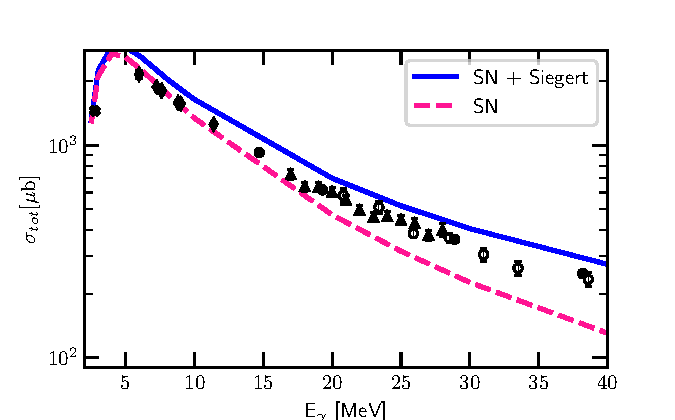
\includegraphics[width=0.75\textwidth]{Figures_De/TOTAL_CROSSSECTION_SMALL_REGION.pdf}
        \end{center}
        \caption{Total cross section $\sigma_{tot}$ for the deuteron photodisintegration process
        as a function of the photon energy E$_\gamma$.
        The solid blue line presents results obtained with \gls{snc}+Siegert 
        and dashed pink line - predictions based on the \gls{snc}.
        In both cases the \gls{sms} \gls{n4lo+} $\Lambda=\SI{450}{\mev}$ force is used.
        The experimental data are from \cite{Bernabei1986} (black filled circles),
        \cite{BOSMAN1979} (empty circles),
        % \cite{ARENDS1984} (squares),
        \cite{Skopik1974} (triangles),
        \cite{Moreh1989} (bold cross "X") and
        \cite{Birenbaum1985} (diamonds).
        }
        \label{TOTAL_CROSS_small}
    \end{figure}

    
    \begin{figure}[htb!]
        \begin{center}
        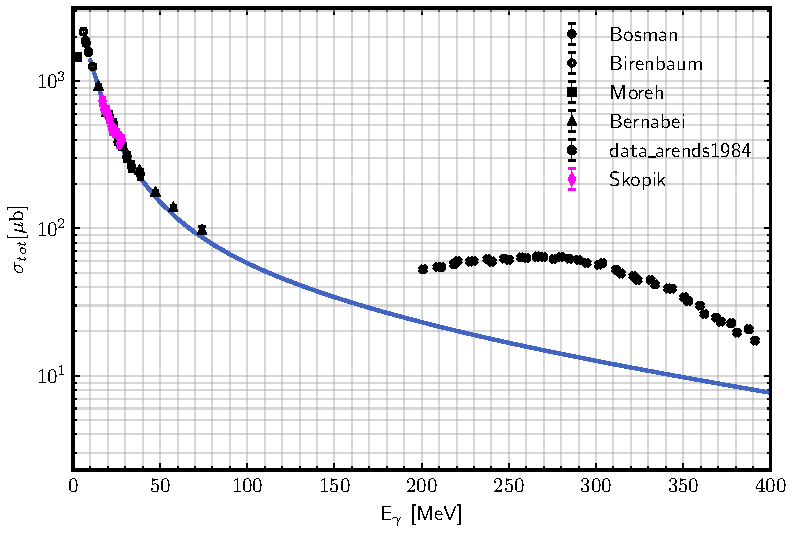
\includegraphics[width=0.75\textwidth]{Figures_De/TOTAL_CROSSSECTION.pdf}
        \end{center}
        \caption{The same as in \fig{TOTAL_CROSS_small} but for the energy range 2.5 - 400 MeV.
        The experimental data are the same as in \fig{TOTAL_CROSS_small}
        but supplemented by the data above $\text{E}_\gamma=\SI{200}{\mev}$ from
        \cite{ARENDS1984} (crosses).
        }
        \label{TOTAL_CROSS}
    \end{figure}

    \begin{figure}[htb!]
        \begin{center}
            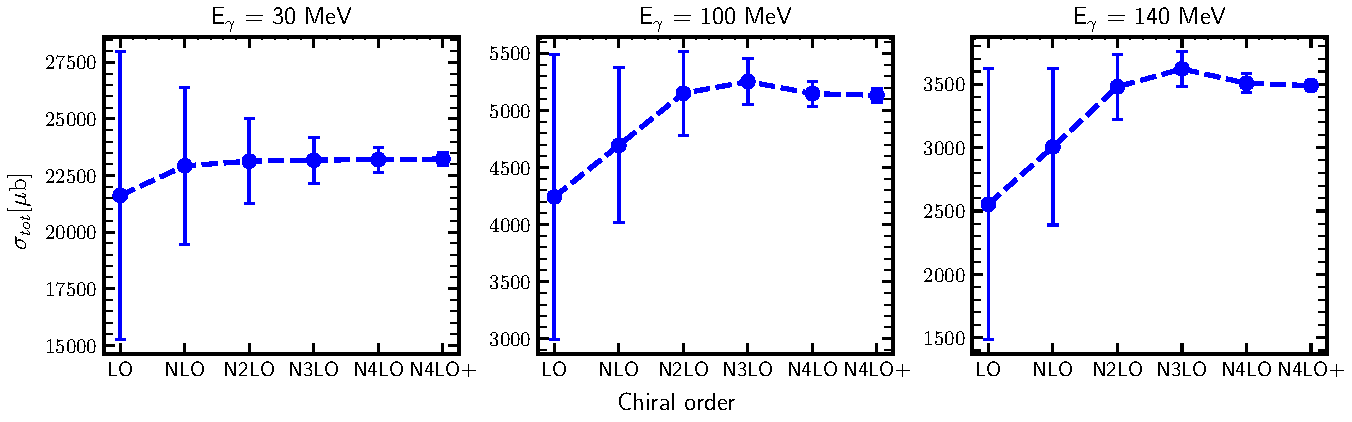
\includegraphics[width=0.95\textwidth]{Figures_De/TOTAL_CROSSSECTION_Truncation.pdf}
        \end{center}
        \caption{Total cross section of the deuteron photodisintegration
        process as a dependence on the chiral order for three photon energy E$_\gamma$ values: \SIlist[list-units = single]{30;100;140}{\mev}.
        Error bands show an estimated truncation error at each order.}
        \label{Trunc_100}
    \end{figure}
    
    In Fig. \ref{Trunc_100} I present the total cross-section for the deuteron photodisintegration 
    at three photon energy values: \SIlist[list-units = single]{30;100;140}{\mev} as a function of the chiral order.
    Error bars show truncation errors calculated using Eq.~\ref{trunc2}~-~\ref{trunc5}.
    One can see that the truncation errors are being reduced with each consecutive chiral order. 
    At \gls{lo} uncertainty is the biggest: \SI{29.46}{\percent} at $\text{E}_\gamma = \SI{30}{\mev}$,
    \SI{29.46}{\percent} at $\text{E}_\gamma = \SI{100}{\mev}$ and
    \SI{41.82}{\percent} at $\text{E}_\gamma = \SI{140}{\mev}$.
    At \gls{n4lo+} it is hardly visible at the presented scale and amounts up to 
    \SI{1.3}{\percent} for each energy(however decreasing with the chiral order).
    For each energy, the prediction is within the uncertainty range at lower orders.
    We see that at lower energy $\sigma_{tot}$ already at NLO reaches valve which remains
    practically unchanged at higher orders.
    Contrarily, at two higher energies, contributions from higher orders are necessary to obtain 
    stable predictions up to approx. \gls{n3lo}.

        
    Figures \ref{Diff_cross_order_pw} and \ref{Diff_cross_err} show my predictions 
    for the differential cross section
    $\frac{d\sigma}{d\Omega}$.
    In both figures, the top, middle, and bottom row shows predictions at 
    $\text{E}_\gamma = \SIlist[list-units = single]{30;100;140}{\mev}$, respectively.
    For all predictions, the contributions of the 2N current are taken into account via the Siegert theorem,
    and unless stated otherwise, I utilize the \gls{sms} \gls{n4lo+} potential.
    The left column of \fig{Diff_cross_order_pw} shows the predictions obtained at 
    different chiral orders (from LO to \gls{n4lo+}) and with $\Lambda=\SI{450}{\mev}$.
    Looking at the best predictions (\gls{n4lo+}, $\Lambda=$~\SI{450}{\mev}) for each
    energy, I
    conclude that the higher the photon energy, the larger 
    difference between the theoretical predictions and experimental 
    data is. At $\text{E}_\gamma = \SI{30}{\mev}$ (top panel) my predictions
    almost perfectly match the data and the difference is almost always
    within the tripled experimental uncertainties. 
    Moving to  $\text{E}_\gamma=\SI{100}{\mev}$ (middle row)
    the description of the data is deteriorating: theoretical
    predictions still match the data qualitatively, but
    the gap for proton emission angle $\theta_p$ in range ($\ang{60} < \theta_p < \ang{130}$) 
    is up to \SI{32}{\percent} (of the predicted value)
    and relative difference (calculated with \eq{eq:relative_diff}) is up to
    \SI{7}{\percent}.
    At the highest energy (bottom row), it is even hard to say about 
    good qualitative description: the general trend of the
    angular dependence is presented, but the predictions are 
    far from the experimental points.
    The relative difference between experimental data and predictions obtained with $N^4LO+$ and $\Lambda=$~\SI{450}{\mev} at \SI{30}{\mev} is less then \SI{13}{\percent}
    and absolute difference is < \SI{3.07}{\micro \barn \per \steradian}.
    At \SI{100}{\mev} discrepancy is larger and the relative difference reaches 46\% with absolute difference up to \SI{1.39}{\micro \barn \per \steradian}.
    Coming to \SI{140}{\mev} the relative difference 
    increases up to \SI{48.6}{\percent} and absolute - \SI{1.93}{\micro \barn \per \steradian}.
    What may be helpful
    for a better data description is a 2N current 
    and relativistic correction mentioned earlier.
    We observe improvements introduced by each subsequent chiral order, but 
    stabilization shows that some ingredients beyond 2N potential are missing.

    The obtained results at each energy confirm the convergence 
    of the predictions concerning the chiral order.
    We see that the cross section at LO is far from both experimental 
    data and the most advanced \gls{n4lo+} predictions, and
    the higher the photon energy, the larger this
    difference is. With each subsequent chiral order, the 
    curves are more closer to each other and the difference
    between \gls{n4lo} and \gls{n4lo+} is hardly visible at the scale used in \fig{Trunc_100}.
    The relative difference between these two predictions at $\text{E}_\gamma=\SI{30}{\mev}$ around the point of maximum 
    ($\theta_p = \ang{80}$) is \SI{0.05}{\percent} which is \SI{0.02}{\micro \barn \per \steradian};
    at \SI{100}{\mev} and $\theta_p = \ang{107}$ it is \SI{0.79}{\percent} (\SI{0.025}{\micro \barn \per \steradian});
    and at \SI{140}{\mev} (same angle) it is \SI{1.8}{\percent} (\SI{0.043}{\micro \barn \per \steradian}).
    Having such small differences between predictions from the two highest chiral orders,
    I can conclude that predictions are converged and 
    using NN potential beyond \gls{n4lo+} chiral orders would rather not bring significant contribution 
    to the cross section values. 
    The difference with experimental data is systematic 
    and is not related to the chiral order. 
    

    Predictions obtained with the \gls{av18} potential 
    (dashed-dotted purple line in the \fig{Diff_cross_order_pw} left)
    are very similar to these from the \gls{n4lo+} \gls{sms} force at lower energies
    (relative difference at $\text{E}_\gamma=\SI{30}{\mev}$ is \SI{0.06}{\percent}
    at the point of maximum $\theta_p = \ang{80}$) and with increasing energy to \SI{140}{\mev}
    it grows up to \SI{3.1}{\percent} at the same scattering angle. 
    It can be connected with our potential's quality loss, but \gls{av18} can
    be struggling with high energies as well.
    That once again shows that other 
    components of Hamiltonian become important at that energies.

    
    In the right column of the \fig{Diff_cross_order_pw} I compare predictions
    based on various assumptions on nuclear current and dynamical mechanism.
    I again use \gls{sms} \gls{n4lo+}, $\Lambda=\SI{450}{\mev}$ force.
    At the lowest energy predictions comprising the plane-wave component only (without rescattering part)
    and taking currents as SNC+Siegert, show relatively small deviation from the full predictions, but the difference increases at larger energies.
    With $\text{E}_\gamma=\SI{30}{\mev}$ the relative difference is \SI{10}{\percent} (\SI{4.03}{\micro \barn \per \steradian})
    at $\theta_p = \ang{80}$. Difference at \SI{100}{\mev} and the same angle is \SI{4}{\percent} (\SI{0.21}{\micro \barn \per \steradian})
    and at \SI{140}{\mev} it is \SI{7}{\percent} (\SI{0.21}{\micro \barn \per \steradian}).
    In contrast, predictions without a two-body current component (1NC) have a much larger gap with a full prediction:
    the difference is \SI{46.5}{\percent} (\SI{13.67}{\micro \barn \per \steradian}) at \SI{30}{\mev},
    \SI{78.6}{\percent} (\SI{2.88}{\micro \barn \per \steradian}) at \SI{100}{\mev} and
    \SI{77.8}{\percent} (\SI{1.68}{\micro \barn \per \steradian}) at \SI{140}{\mev}
    at the same $\theta_p=\ang{80}$.
    Obviously, 2NC contributions are extremely important in this case, the difference connected with them
    is much bigger than theoretical uncertainties or even rescattering contribution.
    For other scattering angles, especially $\theta_p=\ang{0}$ or $\theta_p=\ang{180}$,
    the role of two-body current or FSI is relatively even more pronounced.


    The \fig{Diff_cross_err} (left)
    presents theoretical truncation uncertainties.
    That confirms our expectations
    that for the regarded photo reaction chiral order
    \gls{n4lo+} can produce converged predictions: 
    the black band (representing truncation error at \gls{n4lo+}) is hardly visible
    for the $\text{E}_\gamma=$~\SI{30}{\mev}
    (the relative error for \gls{n4lo+} at \ang{80} is only \SI{0.12}{\percent})
    and is also quite narrow for larger energies (at \SI{140}{\mev} 
    the error at the same angle is \SI{1.46}{\percent}).
    At the lower chiral orders, this band is obviously much wider:
    at \gls{n2lo} it is \SI{1.25}{\percent} at $\text{E}_\gamma=$~\SI{30}{\mev}
    and \SI{15.0}{\percent} at $\text{E}_\gamma=$~\SI{140}{\mev}.
    I note, that the magnitude of the truncation error is only very tiny depending on the scattering angle.
    
    Last but not least, in the right column of \fig{Diff_cross_err}
    I show the cut-off dependence of the differential cross section.
    In the ideal case, that dependence is so weak that
    the choice of the parameter $\Lambda$ would not introduce significant 
    changes. In practice the choice of this parameter is 
    important as it makes a noticeable variation in prediction at higher energies.
    Namely, while at $\text{E}_\gamma=$~\SI{30}{\mev} the cut-off dependence is so tiny
    that, in fact, all the lines (for different $\Lambda$ values)
    overlap each other and we cannot distinguish them with the naked eye:
    the relative difference at the maximum of the cross section is \SI{0.08}{\percent}.
    This is approximately $\frac{2}{3}$ smaller than the truncation error discussed above.
    However, with increasing photon energy up to \SIlist{100; 140}{\mev} 
    (middle and bottom rows of the right column of \fig{Diff_cross_err}) the spread becomes bigger:
    the  uncertainty related to the 
    $\Lambda$-dependence is  \SI{3.35}{\percent} at \SI{100}{\mev}
    and \SI{5.66}{\percent} at \SI{140}{\mev} (the same $\theta_p$).
    Thus at two higher energies, the cut-off dependence becomes more important
    than truncation errors.
    That shows, that proper choice of the $\Lambda$ is important.
    However, if I restrict myself to $\Lambda=\SIlist{450;500}{\mev}$,
    the dependence drops to \SI{1.98}{\percent} at $\text{E}_\gamma=\SI{140}{\mev}$.
    Such a restriction is advocated by a better description of the scattering data
    delivered by the SMS potential for those two values of $\Lambda$.

    In the \fig{Cutoff_dep} we have already seen that the total
    cross section for the same energies has the cut-off spread
    around \SI{4.5}{\percent} for \SI{100}{\mev} and \SI{8}{\percent} for \SI{140}{\mev}
     For $\text{E}_\gamma=\SI{30}{\mev}$ it is below  \SI{1}{\percent}.
     It means that even cut-off dependence for that total cross section (affected
     by the extreme values close to $\theta_p = 0$ or $\theta_p = 180$)  are
     relatively small, especially at the lower energies.


    \begin{figure}[h]
        \centering
        \begin{subfigure}[t]{0.46\textwidth}
            \caption{}
            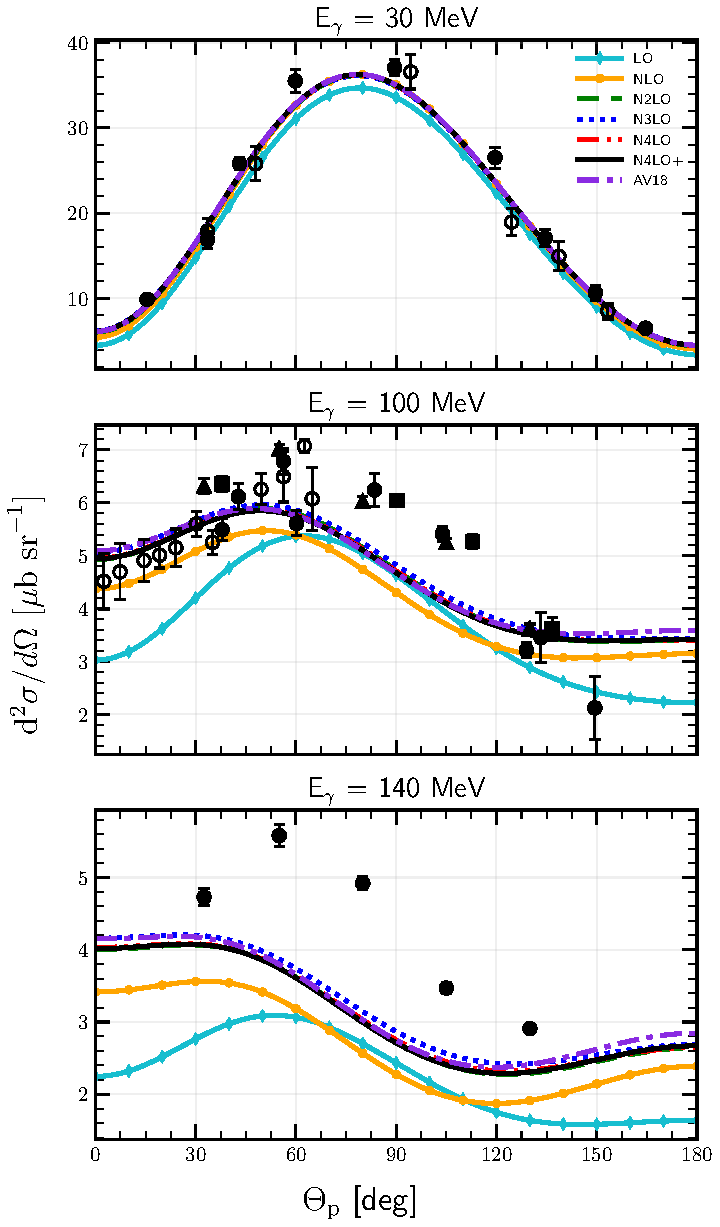
\includegraphics[width=\textwidth]{Figures_De/CROSS2_order_vert.pdf}
            \label{Diff_cross_order}
        \end{subfigure}
        \begin{subfigure}[t]{0.46\textwidth}
            \caption{}
            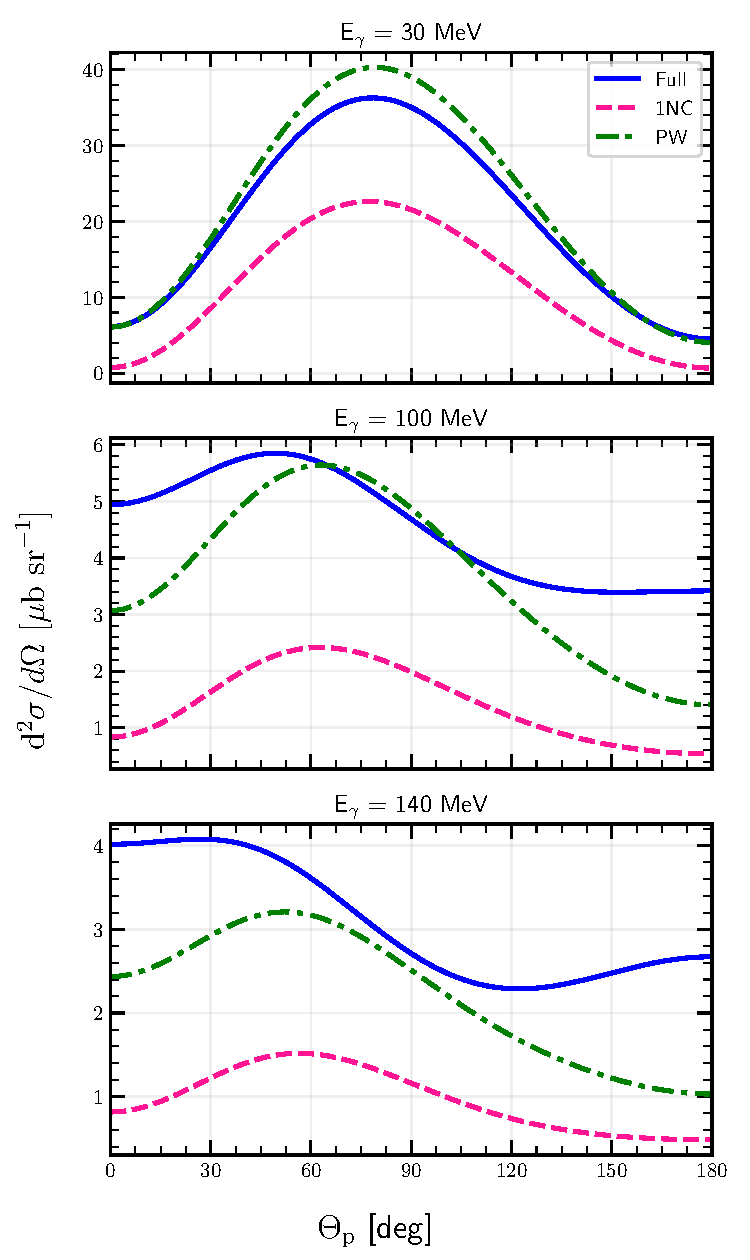
\includegraphics[width=\textwidth]{Figures_De/Diff_cross_pw_1nc.pdf}
            \label{Diff_cross_pw_1nc}
        \end{subfigure}
        \caption{Differential cross section $\frac{d^2\sigma}{d\Omega}$
        as a function of the outgoing proton momentum polar angle $\theta_p$ in the center of mass frame 
        for the photon energy \SI{30}{\mev} (top), \SI{100}{\mev} (middle) and \SI{140}{\mev} (bottom).
        {\bf (a)} Results obtained using the \gls{sms} potential
        at different chiral orders (from LO to \gls{n4lo+}) with the cut-off parameter $\Lambda=\SI{450}{\mev}$ and 
        2NC contributions taken via the Siegert theorem.
        For the sake of comparison, predictions obtained with the \gls*{av18} potential are shown
        by a dashed-dotted purple line.
        Data points (filled and empty circles) are from \cite{Ying_Experiment_Deut}
        for $\text{E}_\gamma=\SIlist[list-units = single]{30; 100}{\mev}$
        and from \cite{DeSanctis_Experiment_Deut} for $\text{E}_\gamma=\SI{140}{\mev}$.
        {\bf (b)} Predictions obtained with the chiral \gls{n4lo+} potential and $\Lambda=\SI{450}{\mev}$
        with various models of nuclear current and scattering state.
        The blue solid curve represents our most complete predictions
        comprising the plane-wave plus rescattering parts and \gls{snc}+Siegert current propagator 
        (the same as \gls{n4lo+} line in (a)).
        The pink dashed curve shows predictions obtained with
        the single-nucleon current only (without applying the Siegert theorem) and the green dashed-dotted
        curve represents predictions with the full current (\gls{snc} + Siegert) but plane-wave part only.
        }
        \label{Diff_cross_order_pw}
    \end{figure}


        
    \begin{figure}[h]
        \centering
        \begin{subfigure}[t]{0.46\textwidth}
            \caption{Truncation error bands.}
            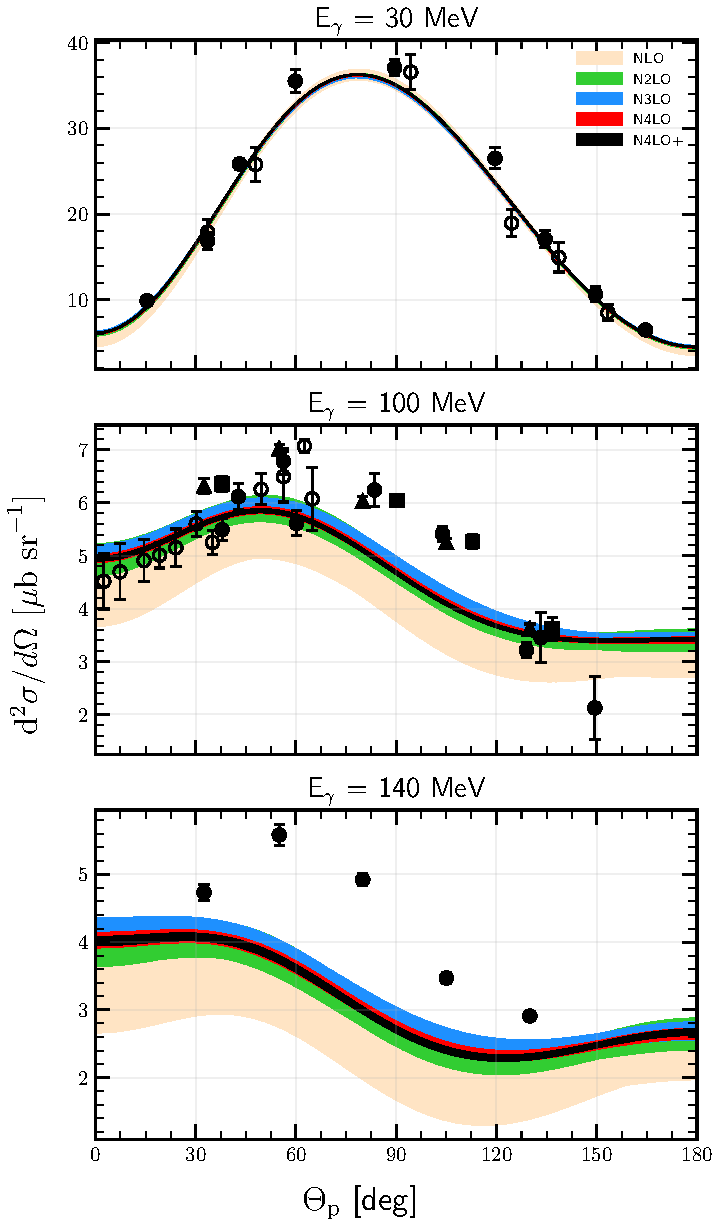
\includegraphics[width=\textwidth]{Figures_De/CROSS2_truncation_vert.pdf}
            \label{Diff_cross_truncation}
        \end{subfigure}
        \begin{subfigure}[t]{0.46\textwidth}
            \caption{Cutoff dependence.}
            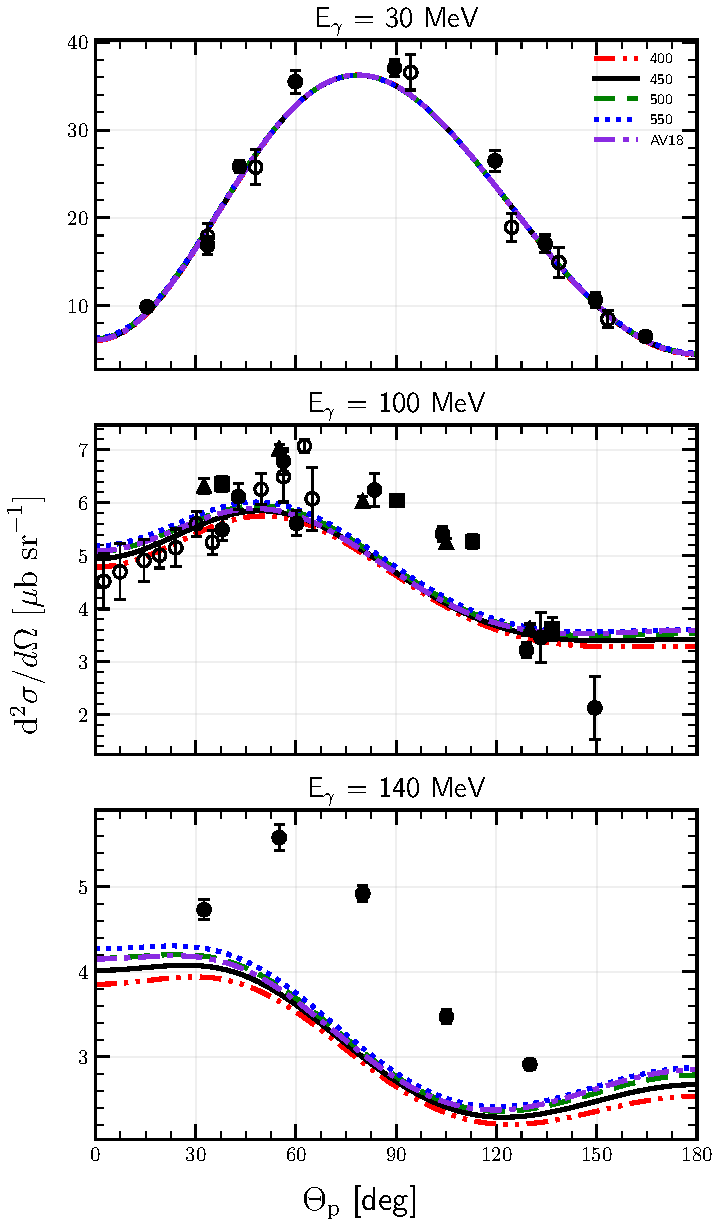
\includegraphics[width=\textwidth]{Figures_De/CROSS2_cutoff_vert.pdf}
            \label{Diff_cross_cutoff}
        \end{subfigure}
        \caption{Theoretical uncertainties 
        for the differential cross section $\frac{d^2\sigma}{d\Omega}$
        as a function of the outgoing proton's momentum polar angle $\theta_p$ in the center of the mass frame 
        for the photon energy is \SI{30}{\mev} (top row), \SI{100}{\mev} (middle row) and \SI{140}{\mev} (bottom row).
        {\bf(a)} The truncation error bands obtained using the \gls{sms} potential
        at different chiral orders (from NLO to \gls{n4lo+}) 
        with the cut-off parameter $\Lambda=\SI{450}{\mev}$ and 2NC contributions taking via the Siegert approach.
        {\bf (b)} Results obtained using different values of the cut-off parameter $\Lambda$.
        The double-dotted-dashed red curve, the solid black line, the dashed green line
        and the dotted blue line represents predictions obtained 
        with $\Lambda=\SIlist[list-units = single]{400;450;500;550}{\mev}$ respectively
        and the chiral potential \gls{n4lo+}. 
        Data points are the same as in \fig{Diff_cross_order}}
        \label{Diff_cross_err}
    \end{figure}

    \clearpage

    \subsection{Polarization observables}
    \label{sec:polarization_results}

    In this subsection, I will present my predictions for the 
    selected polarization observables in the deuteron photodisintegration process
    at two photon energies: $\text{E}_\gamma = \SI{30}{\mev}$ and
    $\text{E}_\gamma = \SI{100}{\mev}$.
    A priori, various polarization states and measurements
    are thinkable for the $\gamma + \text{d}$ scattering.
    Polarization of the target deuteron leads to the deuteron
    analyzing power.
    Similarly using the polarized photons results in the photon asymmetry measurements.
    Using both polarized photon and deuteron allows for spin
    correlation measurement.
    Finally, detecting the spin polarization of at least one nucleon in the final state would deliver
    final polarization or spin transfer coefficients. 
    However, such experiments are very challenging and, up to my best knowledge,
    have not been done yet at regarded here photon energies.
    Thus, in the following, I will restrict myself to results for polarization
    observables arising from the polarization of the initial particles.

    I start with deuteron vector $i\text{T}_{11}$ and tensor $\text{T}_{20}$, $\text{T}_{21}$ and $\text{T}_{22}$
    analyzing power, which arises from various spin states of the deuteron.
    
    Deuteron tensor analyzing powers can be calculated via cross section as it is defined in \cite{rachek2007}:
    
    \begin{eqnarray}
        % \begin{aligned}
            \frac{d \sigma}{d \Omega}= \frac{d \sigma_0}{d \Omega}\left\{1-\sqrt{3 / 4} P_z \sin \theta_H \sin \phi_H T_{11}\right.
            +\sqrt{1 / 2} P_{z z}\left[\left(3 / 2 \cos ^2 \theta_H-1 / 2\right) T_{20}\right. - \nonumber \\
            -\sqrt{3 / 8} \sin 2 \theta_H \cos \phi_H T_{21} 
            \left.\left.+\sqrt{3 / 8} \sin ^2 \theta_H \cos 2 \phi_H T_{22}\right]\right\},
        % \end{aligned}
    \end{eqnarray}
    where $\sigma_0$ is the unpolarized cross section, $P_z$ ($P_{zz}$)
    the vector (tensor) target polarization, $\theta_H$ - the angle
    between polarization axis and photon momentum,
    and $\phi_H$ - is the angle between the polarization plane 
    (containing the polarization axis and momentum of the photon),
    and the reaction plane (containing the momenta of the proton
    and neutron).

    In the Figures \ref{T20_T21_30} (a, b) and \ref{T22_T11_30}(a,b)
    I show my predictions at $\text{E}_\gamma = \SI{30}{\mev}$, for the
    $\text{T}_{20}$, $\text{T}_{21}$, $\text{T}_{22}$  and $i\text{T}_{11}$ respectively as functions 
    of the outgoing proton momentum polar angle $\theta_p$ in the \gls{cm} frame. Each of them
    is organized in a similar way: the top
    panel shows a dependence of the predictions on the 
    chiral order of the potential. The middle subfigure is
    showing a correspondent truncation error for each of the 
    predictions from a top row (except LO, because its uncertainty is
    too large and will spoil the clarity of the figure). The last (bottom)
    panel shows the cut-off dependence at the chiral
    order \gls{n4lo+}. 
    All results have been obtained using \gls{snc}+Siegert model of nuclear current.

    All the analyzing powers presented here show excellent convergence 
    upon a chiral order as it is hard to distinguish the predictions
    from each subsequent order starting from the \gls{n2lo}.
    The relative width of the \gls{n4lo+} truncation band 
    for T$_{20}$, T$_{21}$ and T$_{22}$
    are \SIlist{0.06; 0.05; 0.19}{\percent}, respectively (at $\theta_p=$ \ang{90}, \ang{60} and \ang{90}, respectively).
    The slowest convergence is observed for $i\text{T}_{11}$ (\fig{T11_30_vert})
    where we can recognize \gls{n2lo} band in the figure.
    Nevertheless, at the \gls{n4lo+}
    the width truncation band at $\theta_p = \ang{20}$ (maximum point)
    is only a \SI{0.2}{\percent}.
    The cut-off dependence for all regarded observables is weak and 
    predictions for each value of the $\Lambda$ are hardly separable 
    with the naked eye.
    The relative spread of the predictions based on various $\Lambda$ at the same angles as above 
    are \SIlist{0.87; 0.94; 3.42; 0.68}{\percent} for T$_{20}$, T$_{21}$, T$_{22}$ and $i\text{T}_{11}$, respectively.


    Corresponding predictions at the photon energy $\text{E}_\gamma = \SI{100}{\mev}$
    (Figs. \ref{T20_T21_100} and \ref{T22_T11_100}) preserve similar
    trends for each observable. 
    In general, predictions are being converged starting
    even from the \gls{n2lo} and only for the $i\text{T}_{11}$
    I find
    that truncation error's bands are noticeably wide
    even at \gls{n4lo} and \gls{n4lo+}.
    Cutoff dependence at this energy is a bit stronger
    compared to those at $\text{E}_\gamma = \SI{30}{\mev}$, especially
    for 
    $\text{T}_{22}$ and $i\text{T}_{11}$ analyzing powers (\fig{T22_T11_100} vs \fig{T22_T11_30}),
    where one can see 
    the slightly stronger discrepancy at the maxima and minima points.
    
    The choice of $\Lambda$ does not affect predictions substantially
    even at that higher energy:
    the relative spread among all cut-offs for T$_{20}$ is \SI{1.54}{\percent}
    around the point of maximum ($\theta_p = \ang{90}$).
    For other components of the tensor analyzing power spread amounts up to:
    \SI{0.14}{\percent} at $\theta_p = \ang{60}$ for T$_{21}$;
    \SI{3.68}{\percent} at $\theta_p = \ang{90}$ for T$_{22}$;
    and \SI{4.91}{\percent} at $\theta_p = \ang{75}$ for $i\text{T}_{11}$.
    We see again that $i\text{T}_{11}$ has much larger spread in the maximum and
    is more sensitive to the cut-off choice.
    However, summarizing my findings 
    for the deuteron tensor analyzing powers,
    I conclude that cut-off dependence is generally weak
    also at $\text{E}_\gamma = \SI{100}{\mev}$.

    Turning our attention to the chiral order convergence, we
    observe that predictions are mostly converged starting either from \gls{n2lo} or \gls{n3lo}.
    The relative width of \gls{n4lo+} truncation band 
    for T$_{20}$, T$_{21}$ and T$_{22}$
    are \SIlist{0.7; 0.7; 0.04}{\percent} respectively (at the same angles as used above).
    Another case is $i\text{T}_{11}$, for which this width is much larger: \SI{6.8}{\percent} at $\theta_p = \ang{20}$.
    The truncation uncertainty for all analyzing powers is much lower than one,
    related to the choice of the cut-off parameter.
    However, $i\text{T}_{11}$ seems to be more sensitive both
    to the choice of the cut-off parameter and to the chiral order than other regarded observables.
    Even for $i\text{T}_{11}$, the cut-off spread is almost twice larger than the truncation error.
    Standing out of other tensor components, $i\text{T}_{11}$ can be useful for the investigation of 
    the cut-off dependence of the model.
    Of course, we can repeat once more that 
    our model is less accurate at higher energies which is reflected
    in a stronger cut-off dependence and slower chiral convergence.
    However, I conclude that even at these energies tensor analyzing powers are
    well converged with respect to the chiral order.

    Comparison of the predictions obtained using the chiral \gls{n4lo+} potential
    $\Lambda = \SI{450}{\mev}$ with ones obtained taking \gls{av18} potential
    show a very good agreement: the relative difference at $\text{E}_\gamma=\SI{30}{\mev}$
    is below \SI{6}{\percent} for the regarded tensor analyzing powers at specified angles.
    Picture at  $\text{E}_\gamma=\SI{100}{\mev}$ is even better: the difference does not exceed 
    \SI{4}{\percent} for all observables and a whole range of scattering angles.


    \begin{figure}[htb]
        \centering
        \begin{subfigure}[b]{0.46\textwidth}
            \caption{T$_{20}$}
            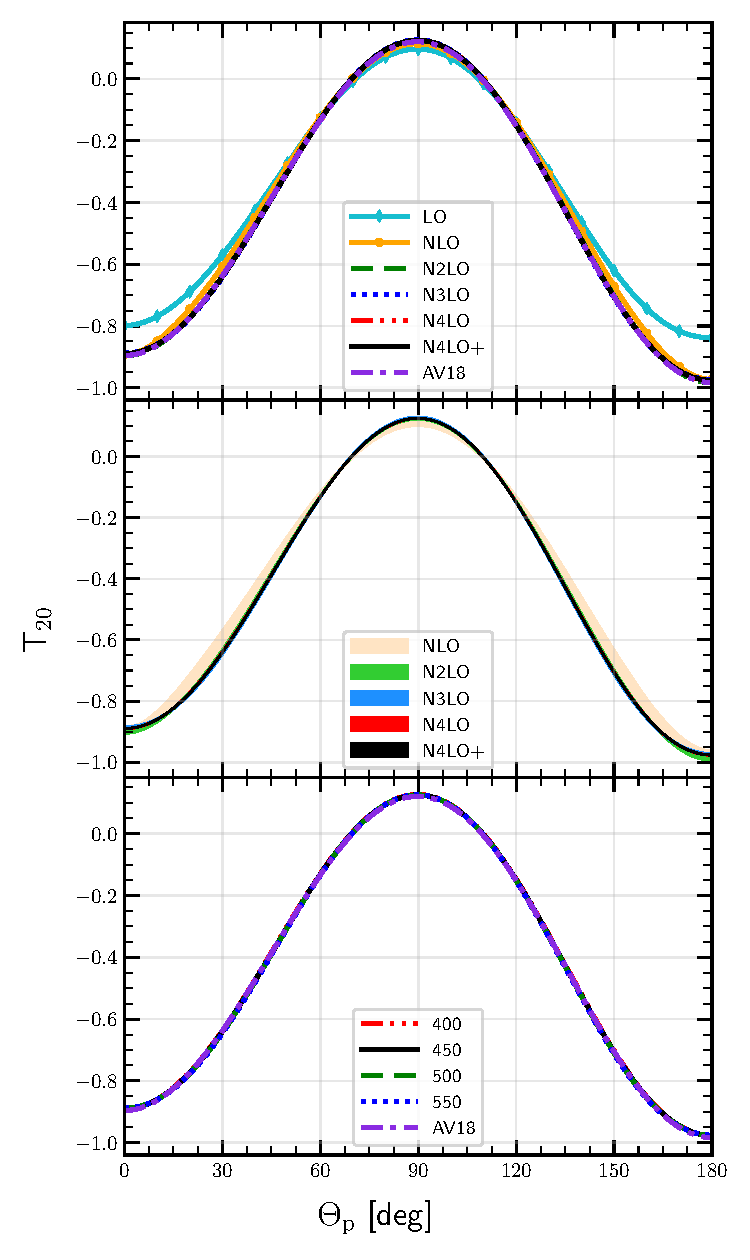
\includegraphics[width=\textwidth]{Figures_De/T20D2_30mev.pdf}
            \label{T20_30_vert}
        \end{subfigure}
        \begin{subfigure}[b]{0.46\textwidth}
            \caption{T$_{21}$}
            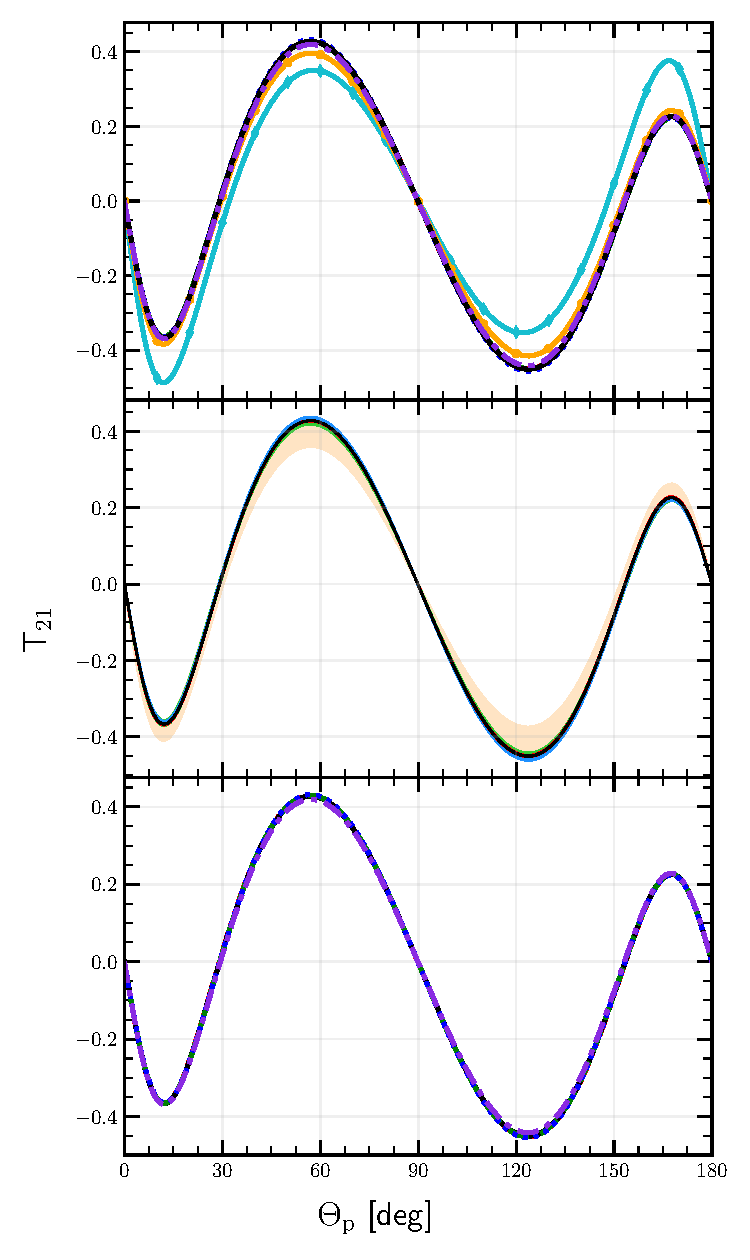
\includegraphics[width=\textwidth]{Figures_De/T21D2_30mev.pdf}
            \label{T21_30_vert}
        \end{subfigure}
        \caption{The deuteron tensor analyzing powers T$_{20}$  {\bf (a)}
        and T$_{21}$ {\bf (b)}
        as a function of the outgoing proton angle $\theta_p$ in the \glsxtrlong{cm} frame 
        for the photon energy $\text{E}_\gamma = \SI{30}{\mev}$.
        The top row presents results obtained using the \gls{sms} potential
        at different chiral orders (from LO to \gls{n4lo+}) with the cut-off parameter $\Lambda=\SI{450}{\mev}$.
        The middle row shows truncation errors for each 
        chiral order starting from NLO and
        the bottom row presents a cut-off dependence at \gls{n4lo+}.
        For the sake of comparison, predictions obtained with the \gls{av18} potential are given as well.
        For all predictions \gls{snc}+Siegert model is used.}
        \label{T20_T21_30}
    \end{figure}

    \begin{figure}[htb]
        \centering
        \begin{subfigure}[b]{0.46\textwidth}
            \caption{T$_{22}$}
            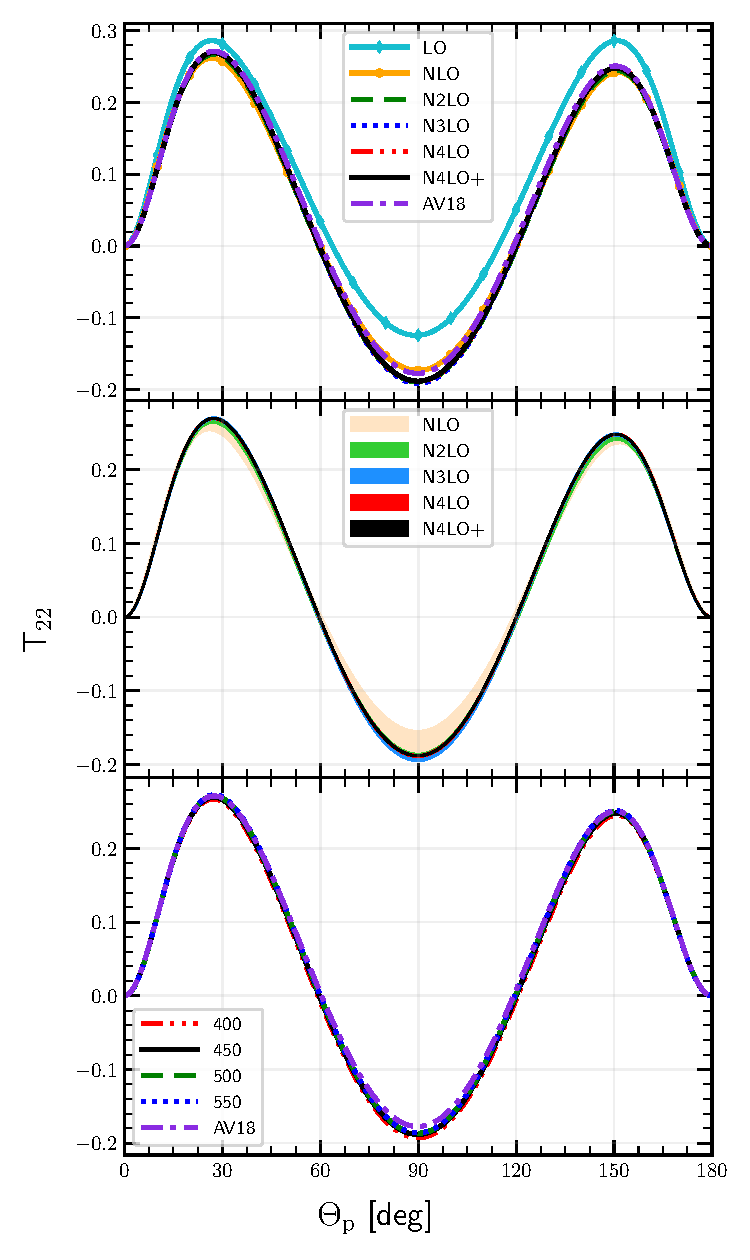
\includegraphics[width=\textwidth]{Figures_De/T22D2_30mev.pdf}
            \label{T22_30_vert}
        \end{subfigure}
        \begin{subfigure}[b]{0.46\textwidth}
            \caption{$i\text{T}_{11}$}
            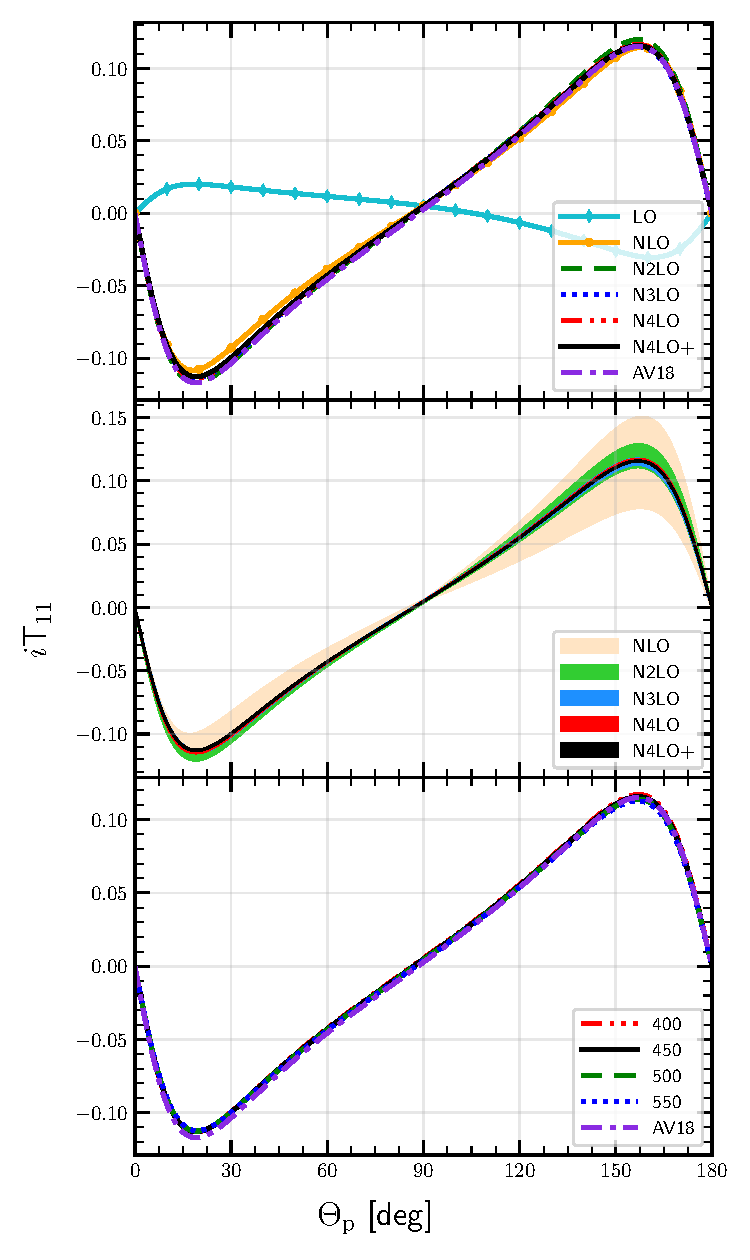
\includegraphics[width=\textwidth]{Figures_De/T11D2_30mev.pdf}
            \label{T11_30_vert}
        \end{subfigure}
        \caption{The same as in \fig{T20_T21_30} but for the deuteron tensor analyzing power
        T$_{22}$ (left column {\bf (a)}) and the deuteron vector analyzing power
        $i\text{T}_{11}$ (right column  {\bf (b)}).}
        \label{T22_T11_30}
    \end{figure}

    \begin{figure}[htb]
        \centering
        \begin{subfigure}[b]{0.46\textwidth}
            \caption{T$_{20}$}
            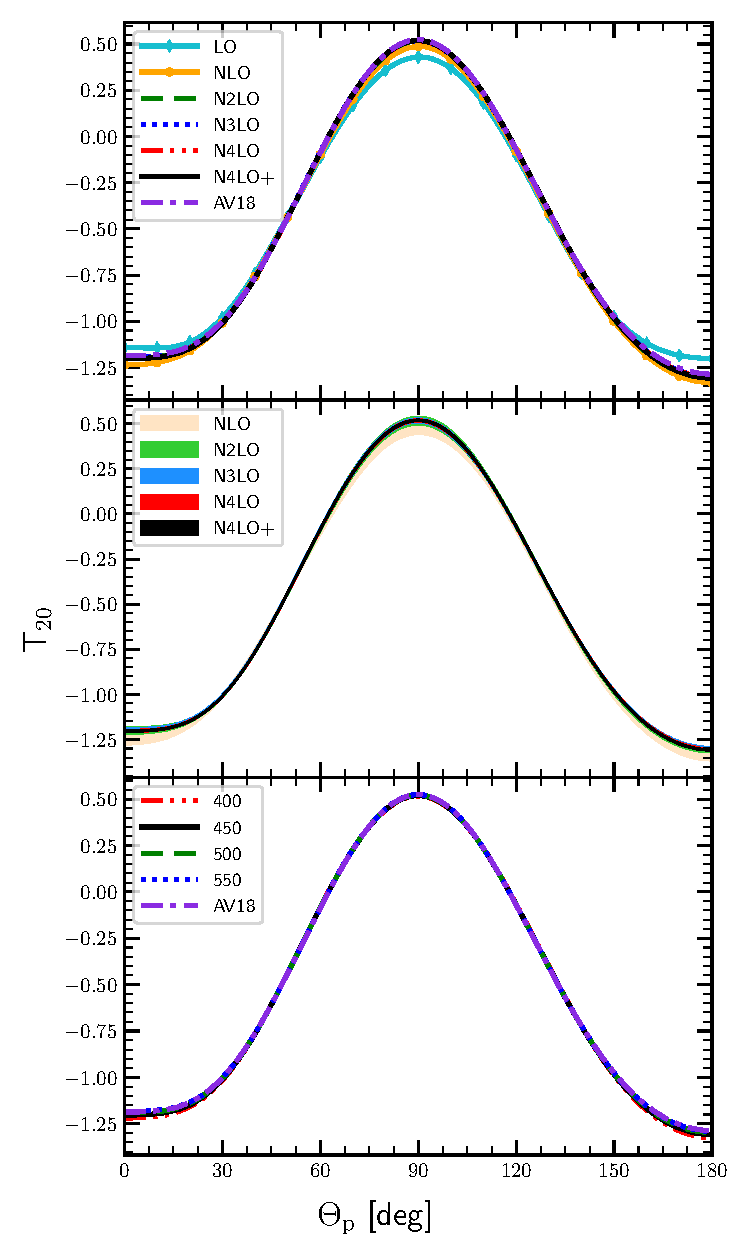
\includegraphics[width=\textwidth]{Figures_De/T20D2_100mev.pdf}
            \label{T20_100_vert}
        \end{subfigure}
        \begin{subfigure}[b]{0.46\textwidth}
            \caption{T$_{21}$}
            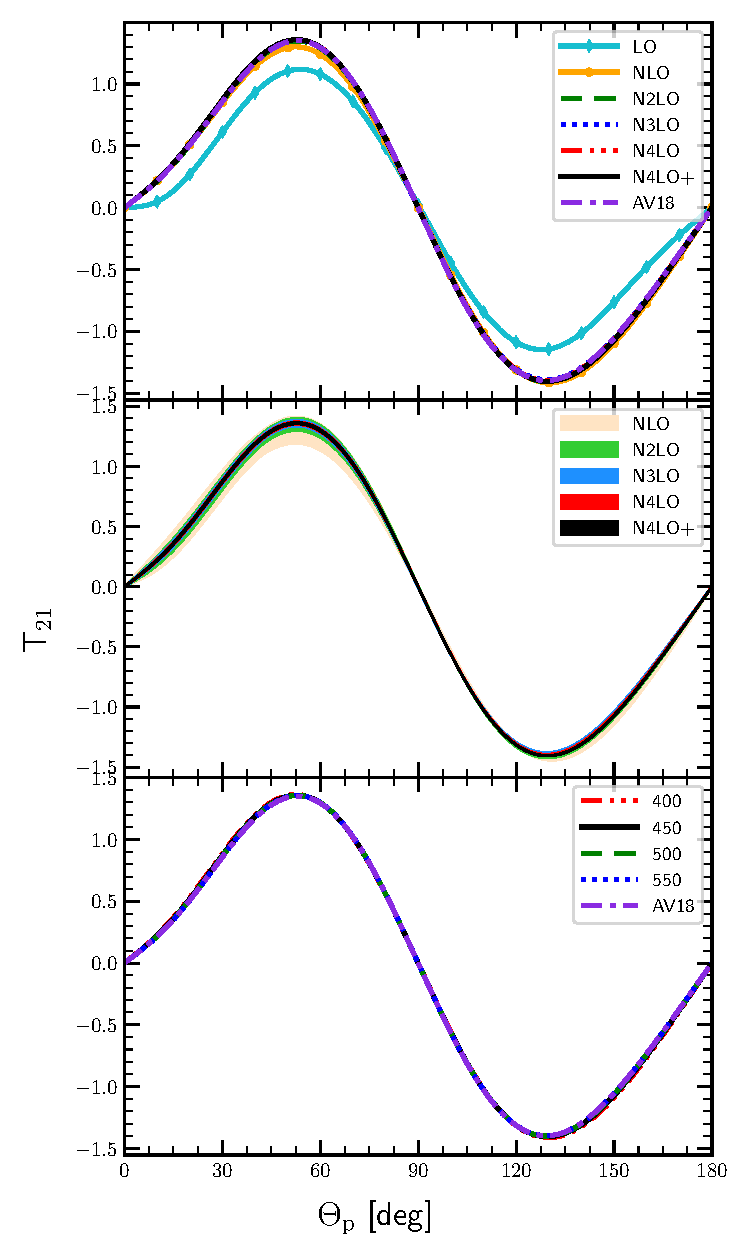
\includegraphics[width=\textwidth]{Figures_De/T21D2_100mev.pdf}
            \label{T21_100_vert}
        \end{subfigure}
        \caption{The deuteron tensor analyzing powers T$_{20}$  {\bf (a)}
        and T$_{21}$ {\bf (b)}
        as a function of the outgoing proton angle $\theta_p$ in the center of mass frame 
        for the photon energy E$_\gamma=\SI{100}{\mev}$.
        The top row presents results obtained using the \gls{sms} potential
        at different chiral orders (from \gls{lo} to \gls{n4lo+}) with the cut-off parameter $\Lambda=\SI{450}{\mev}$.
        The middle row shows truncation errors for each 
        chiral order starting from \gls{nlo} and the
        bottom row presents a cut-off dependence at \gls{n4lo+}.
        For the sake of comparison, predictions obtained with the \gls{av18} potential are given as well.
        For all predictions \gls{snc}+Siegert model is used.}
        \label{T20_T21_100}
    \end{figure}

    \begin{figure}[htb]
        \centering
        \begin{subfigure}[b]{0.46\textwidth}
            \caption{T$_{22}$}
            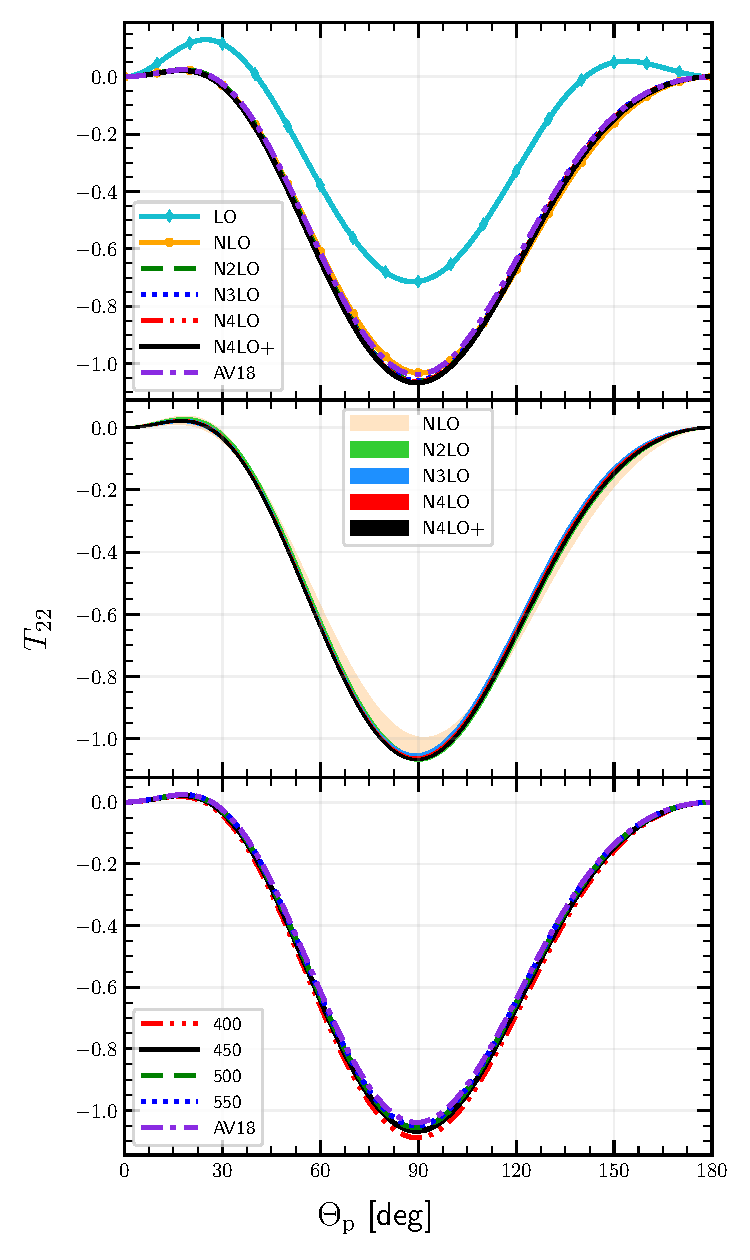
\includegraphics[width=\textwidth]{Figures_De/T22D2_100mev.pdf}
            \label{T22_100_vert}
        \end{subfigure}
        \begin{subfigure}[b]{0.46\textwidth}
            \caption{$i\text{T}_{11}$}
            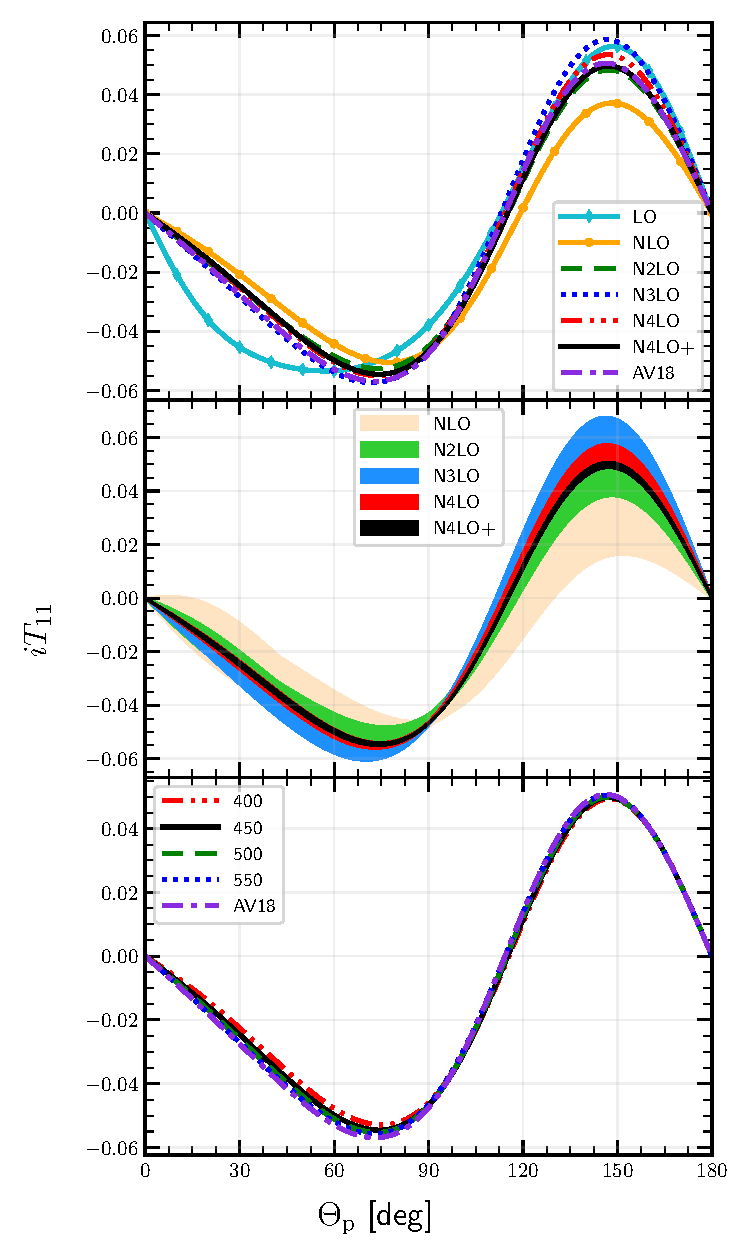
\includegraphics[width=\textwidth]{Figures_De/T11D2_100mev.pdf}
            \label{T11_100_vert}
        \end{subfigure}
        \caption{The same as in \fig{T20_T21_100} but for the deuteron tensor analyzing power
        T$_{22}$ (left column {\bf (a)}) and
        the deuteron vector analyzing power $i\text{T}_{11}$
        (right column {\bf (b)}).}
        \label{T22_T11_100}
    \end{figure}

    In \fig{tensor_pw_1nc} together with our most advanced "Full" predictions 
    (\gls{n4lo+}, $\Lambda=\SI{450}{\mev}$, the Siegert theorem),
    at $\text{E}_\gamma = \SI{30}{\mev}$ 
    I show predictions obtained with 1NC only and 
    the Siegert predictions but with plane-wave contribution without rescattering part.
    In the case of deuteron's tensor analyzing power components, the contribution of rescattering part is  
    important for T$_{20}$, T$_{21}$ and T$_{22}$ (the relative difference is up to \SI{20}{\percent} 
    in extremes).
    and crucial for
    $i\text{T}_{11}$ where the PW part equals to zero.
    The 2NC component taken into account via Siegert theorem has a dominant contribution here. We see that 
    1NC predictions are absolutely away from the "Full" predictions and in the case of $i\text{T}_{11}$
    does not even reflect complete prediction qualitatively.

    \begin{figure}[h]
        \begin{center}
        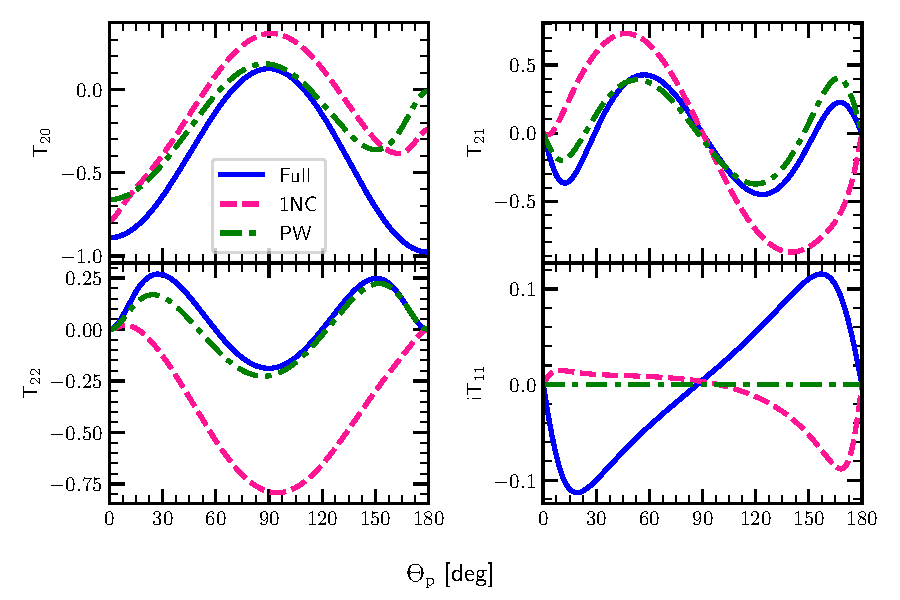
\includegraphics[width=0.9\textwidth]{Figures_De/TensorPowers_pw_1nc.pdf}
        \end{center}
        \caption{The deuteron tensor analyzing powers T$_{20}$, T$_{21}$, T$_{22}$ and 
        the deuteron vector analyzing power $i\text{T}_{11}$ as a function of the
        outgoing proton angle $\theta_p$ in the \gls{cm} frame at $\text{E}_\gamma = \SI{30}{\mev}$.
        Similarly to \fig{Diff_cross_pw_1nc} predictions obtained with chiral \gls{n4lo+} potential
        and $\Lambda=\SI{450}{\mev}$ are presented for three theoretical models.
        The blue solid line is the most complete prediction we have (plane-wave plus rescattering parts, 1NC + Siegert), the pink dashed line shows predictions obtained with
        single-nucleon current only (1NC) - without the Siegert contributions and the green dashed-dotted line
        is a prediction in which we neglect the rescattering part
        and stick to the plane-wave part only but keeping the Siegert contributions.}
        \label{tensor_pw_1nc}
    \end{figure}

    \fig{tensor_pw_1nc_100mev} presents similar results but for E$_\gamma = \SI{100}{\mev}$
    and it is interesting that the difference between Full and 1NC prediction becomes smaller
    and it is especially visible for $\text{T}_{22}$. At this energy, the relative difference 
    between "Full" and 1NC predictions
    at $\theta_p = \ang{90}$ is \SI{43.6}{\percent} compared to \SI{122.8}{\percent}
    at E$_\gamma = \SI{30}{\mev}$. Similarly, the difference for T$_{20}$
    at E$_\gamma = \SI{30}{\mev}$($\theta_p = \ang{90}$) is \SI{91.4}{\percent}
    and at E$_\gamma = \SI{100}{\mev}$ it drops to \SI{28.8}{\percent}.
    This may also be affected by the fact that values at $\theta_p = \ang{90}$ 
    are quite small for the Full prediction, nevertheless, the difference still becomes smaller at the
    E$_\gamma = \SI{100}{\mev}$.
    This trend is noticeable by looking also on the results presented below.
    Nevertheless, in both cases 2NC (via the Siegert) brings sufficient contributions
    and cannot be omitted for obtaining the full picture.

    \begin{figure}[h]
        \begin{center}
        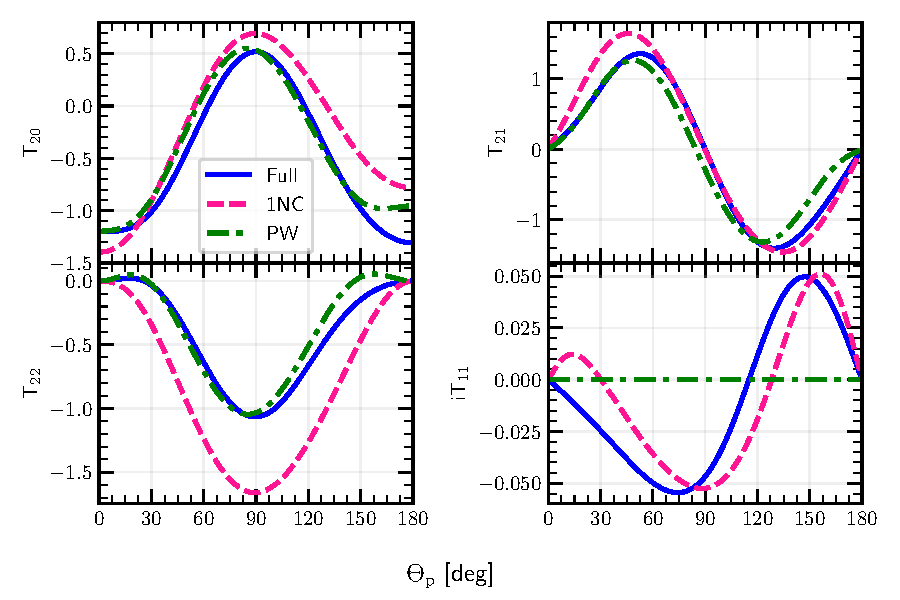
\includegraphics[width=0.9\textwidth]{Figures_De/TensorPowers_100mev_pw_1nc.pdf}
        \end{center}
        \caption{The same as in \fig{tensor_pw_1nc} but for E$_\gamma=\SI{100}{\mev}$.}
        \label{tensor_pw_1nc_100mev}
    \end{figure}

    
    In the following figures, I will compare my predictions with experimental data.
    In some cases, I will keep a similar way as it was done
    in \cite{rachek2007} where due to experimental conditions results are given not at single photon energy,
    but for a specific ranges of $\text{E}_\gamma$.
    In the Figures \ref{tensor_angular_25-45} - \ref{tensor_angular_230-330}
    I show an angular dependence of the $\text{T}_{2i}$ ($i=0,1,2$) for a specific energy bands:
    \SIrange[range-phrase=--]{25}{45}{\mev}, \SIrange[range-phrase=--]{45}{70}{\mev},
    \SIrange[range-phrase=--]{70}{100}{\mev}, and \SIrange[range-phrase=--]{230}{330}{\mev}.
    The solid blue line shows an average value of the observable in the specified energy intervals:
    obtained at \gls{n4lo+} with $\Lambda=\SI{450}{\mev}$, while the pink dashed line is a prediction
    obtained with the same setup but without using contributions from Siegert approach
    (single nucleon current only). Bands for each prediction specify the spread of
    predictions due to the energy band.
    
    One clearly sees that the data description is better for the predictions with Siegert contributions included
    and the \gls{snc} alone is not able to describe the experiment properly.
    Our Full model nicely describes data up to $\text{E}_\gamma = \SI{70}{\mev}$.
    With increasing energy (above \SI{100}{\mev}),
    the difference between predicted values and experimental data becomes larger
    (especially for $\text{T}_{22}$), 
    which shows a necessity of improving the theoretical model before applying it to 
    higher energies. Nevertheless, even with approximations used,
    the data description remains reasonable. 
    We observe that quite often and in particular in \fig{tensor_angular_180-230} and \fig{tensor_angular_230-330}
    the data description is worse for smaller angles. Especially for the tensor analyzing power T$_{22}$
    the group of data point lying closer to $\theta_p = \ang{30}$ are farther 
    from the theoretical prediction than second group.
    In \fig{tensor_angular_230-330} the description of data points for T$_{20}$ seem to be better
    with the \gls{snc} (dashed line), but in this case, it is only an accidental match as we do not observe similar rend for any other angular range or for different observables.
    In addition, experimental uncertainties are larger at small angles, and in all cases 
    our description is inside 3$\sigma$ uncertainty.
    




    \begin{figure}[h]
        \begin{center}
        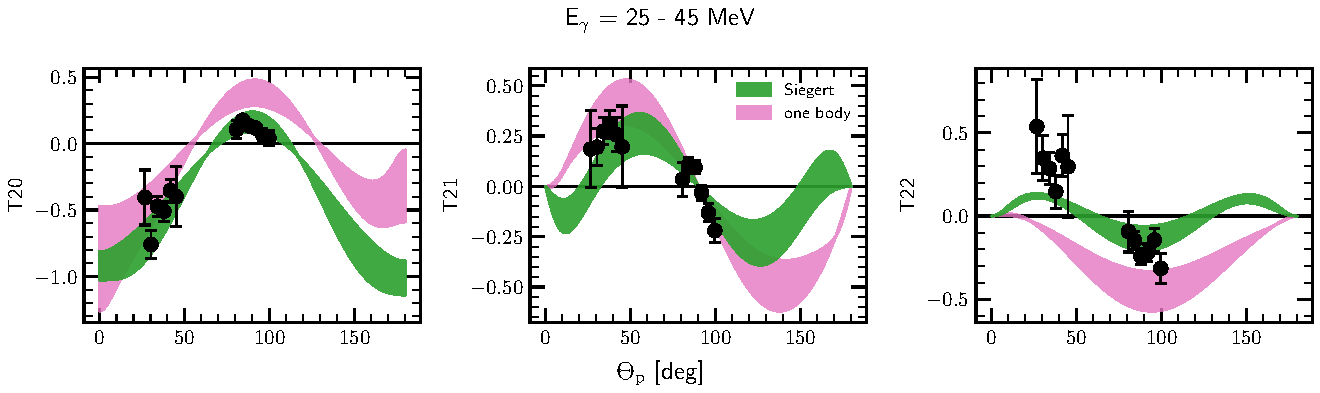
\includegraphics[width=1\textwidth]{Figures_De/Tensor_analyzing_power_angular_E25-45.pdf}
        \end{center}
        \caption{Tensor analyzing powers T$_{20}$, T$_{21}$ and T$_{22}$ as a function of the
        outgoing proton angle $\theta_p$ in the \gls{cm} frame.
        The solid blue line is the mean value of my predictions obtained 
        at energy values from \SIrange[range-phrase=\text{ to }]{25}{45}{\mev} with the
        \gls{sms} potential at \gls{n4lo+} chiral order and with $\Lambda$~=~450~MeV
         and with \gls{snc} used together with the Siegert approach. 
        The pink dashed line is a similar prediction but with the \gls{snc} only. 
        The corresponding bands show the limits of predictions in the regarded
        energy region.
        Filled circles are experimental data
        from \cite{rachek2007} for the same energy range.}
        \label{tensor_angular_25-45}
    \end{figure}

    \begin{figure}[h]
        \begin{center}
        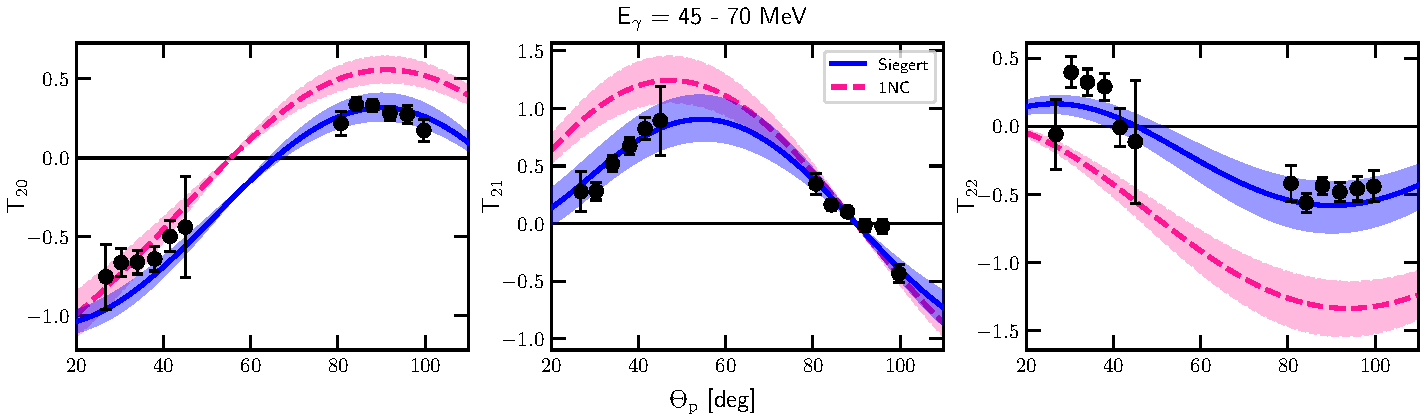
\includegraphics[width=0.95\textwidth]{Figures_De/Tensor_analyzing_power_angular_E45-70.pdf}
        \end{center}
        \caption{The same as in \fig{tensor_angular_25-45} but for energy bin \SIrange{45}{70}{\mev}.}
        \label{tensor_angular_45-70}
    \end{figure}

    \begin{figure}[h]
        \begin{center}
        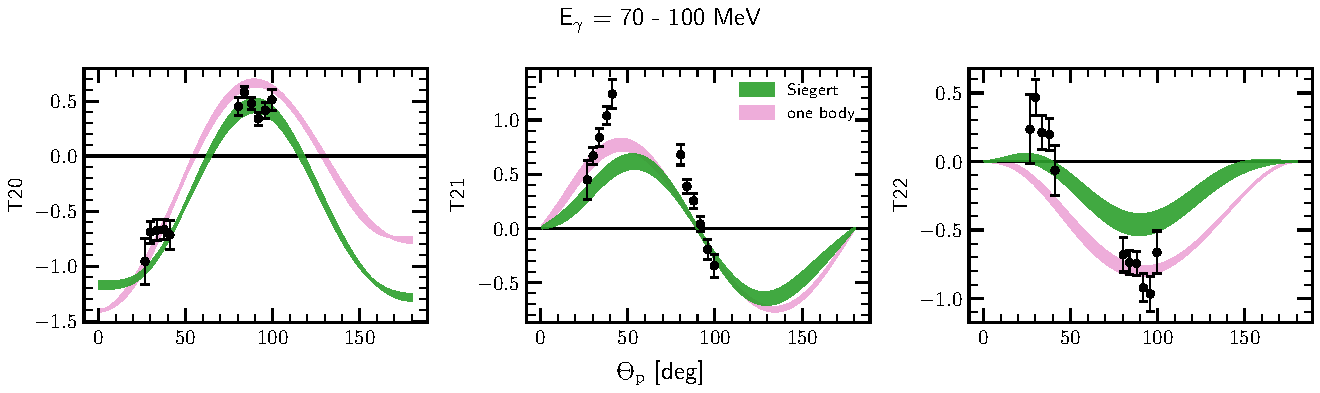
\includegraphics[width=0.95\textwidth]{Figures_De/Tensor_analyzing_power_angular_E70-100.pdf}
        \end{center}
        \caption{The same as in \fig{tensor_angular_25-45} but for energy bin \SIrange{70}{100}{\mev}.}
        \label{tensor_angular_70-100}
    \end{figure}        

    \begin{figure}[h]
        \begin{center}
        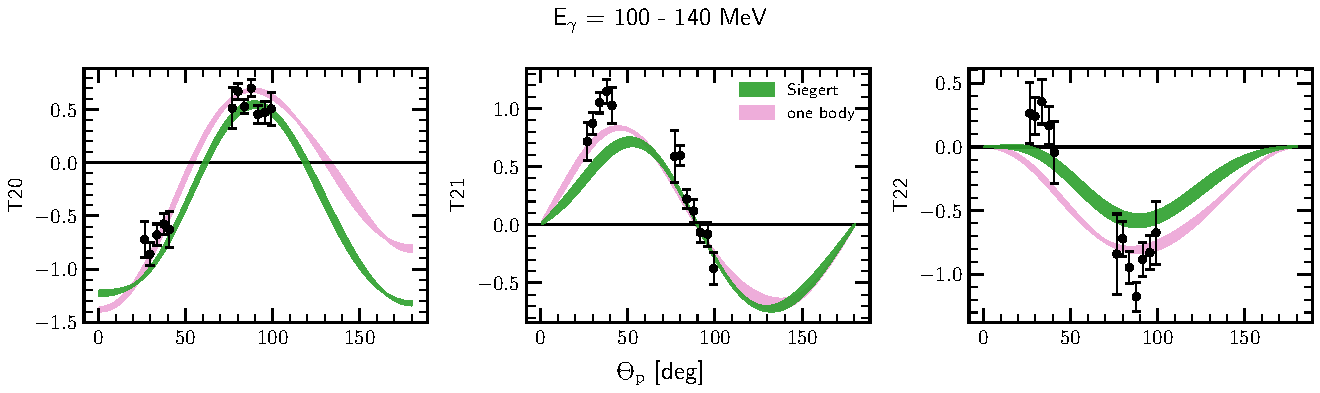
\includegraphics[width=0.95\textwidth]{Figures_De/Tensor_analyzing_power_angular_E100-140.pdf}
        \end{center}
        \caption{The same as in \fig{tensor_angular_25-45} but for energy bin \SIrange{100}{140}{\mev}.}
        \label{tensor_angular_100-140}
    \end{figure}
        
        

    \begin{figure}[h]
        \begin{center}
        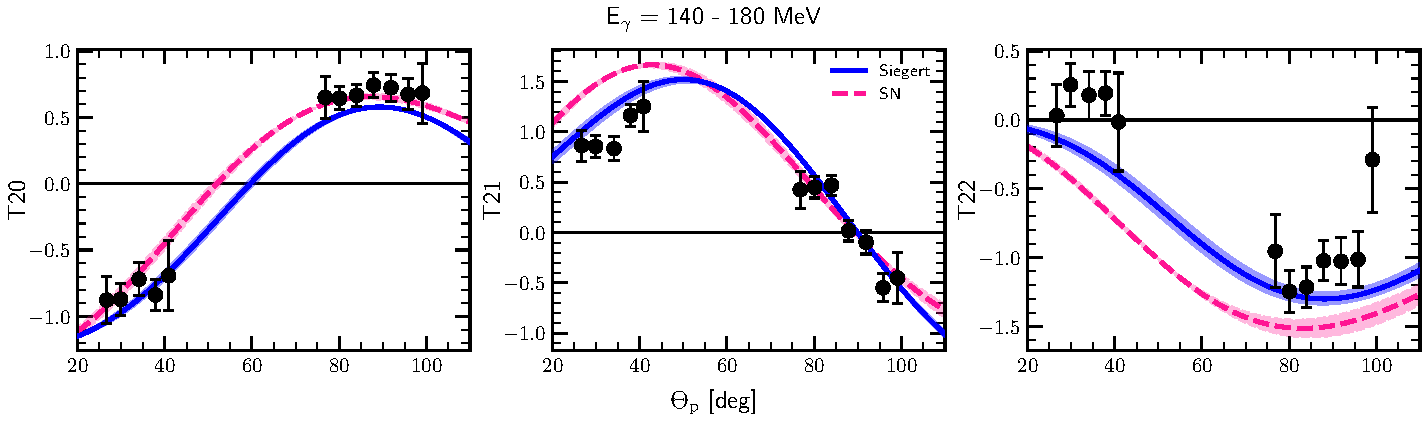
\includegraphics[width=0.95\textwidth]{Figures_De/Tensor_analyzing_power_angular_E140-180.pdf}
        \end{center}
        \caption{The same as in \fig{tensor_angular_25-45} but for energy bin \SIrange{140}{180}{\mev}}
        \label{tensor_angular_140-180}
    \end{figure}
        

    \begin{figure}[h]
        \begin{center}
        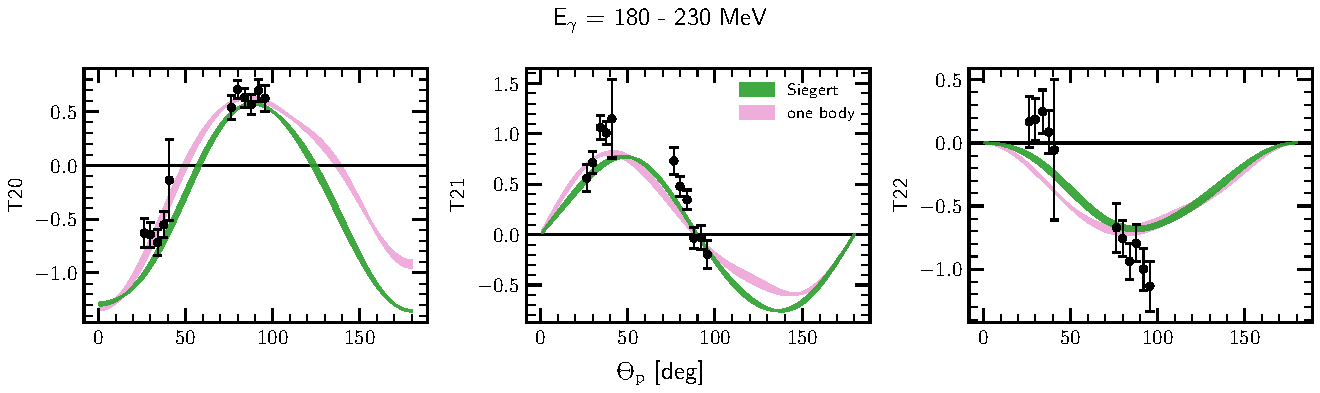
\includegraphics[width=0.95\textwidth]{Figures_De/Tensor_analyzing_power_angular_E180-230.pdf}
        \end{center}
        \caption{The same as in \fig{tensor_angular_25-45} but for energy bin \SIrange{180}{230}{\mev}}
        \label{tensor_angular_180-230}
    \end{figure}

    \begin{figure}[h]
        \begin{center}
        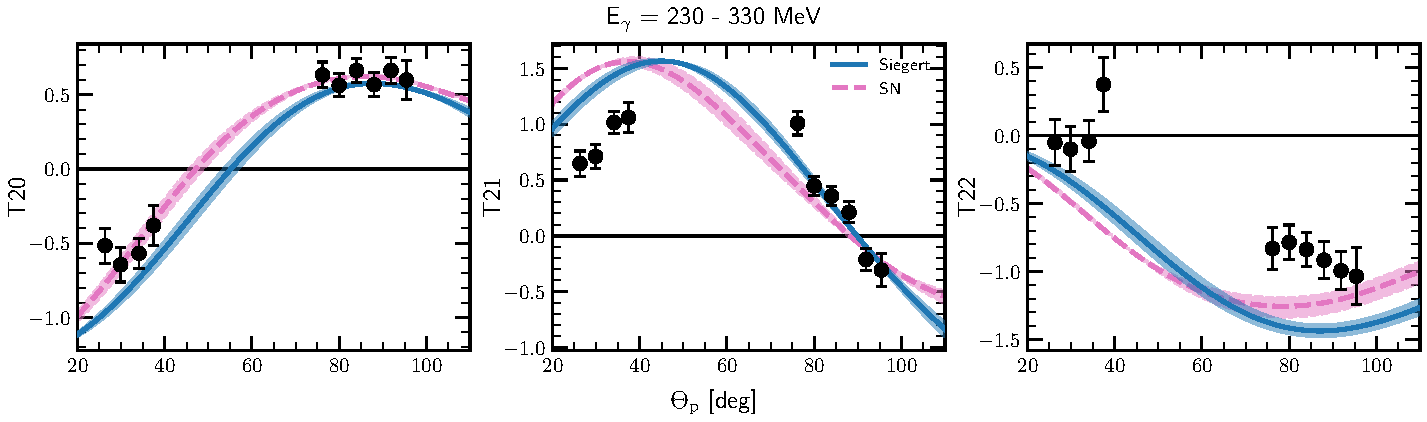
\includegraphics[width=0.95\textwidth]{Figures_De/Tensor_analyzing_power_angular_E230-330.pdf}
        \end{center}
        \caption{The same as in \fig{tensor_angular_25-45} but for energy bin \SIrange{230}{330}{\mev}}
        \label{tensor_angular_230-330}
    \end{figure}
        


    In the Figure \ref{T20_vs_en} the energy dependence of $\text{T}_{20}$ and $\text{T}_{22}$
    at specific angle $\theta_p = \ang{88}$
    is presented for the energy range 0-400~MeV. Besides my predictions I also demonstrate the experimental data from
    \cite{rachek2007} and \cite{mishev1993} as well as theoretical calculations from \cite{Schmitt1989}.
    For $\text{T}_{20}$ all models are able to describe experimental data well even for
    high energies. On the other hand, $\text{T}_{22}$ is not described so well: for the 
    energies below \SI{140}{\mev} the predictions are within uncertainties of experimental data,
    but further the difference with the data increases. Above \SI{140}{\mev}
    Full predictions do not  
    reflect the qualitative nature of the data. Namely, I observe that
    data points start ascending which is not represented in my predictions.
    Theoretical predictions from \cite{Schmitt1989} (brown dashed curve) are also not able
    to describe data quantitatively for $\text{T}_{22}$, but increasing of T$_{22}$
    towards data is present. The predictions in \cite{Schmitt1989}
    are obtained with a one-body current using the Bonn one-boson-exchange potential
    in coordinate space (OBEPR)
    NN potential with the major part of meson exchange
    currents (MEC) included implicitly via the Siegert operators plus explicit
    pion exchange currents (MEC), isobar configurations
    (IC) and the leading order of relativistic corrections
    (RC). So authors use a different potential, but
    probably the main difference in predictions is coming from the
    more advanced model of the current operator
    and the RC included there.
    We see that experimental errors are quite large which is not so surprising
    giving that the experiment was conducted back in 1989.
    New experiments would be a great support in development of the nuclear interactions
    as we expect relativistic calculations in the future \cite{Grassi2023}.

    The \fig{T20_vs_en_cutoff} presents similar results to the \fig{T20_vs_en} but
    with various values of the cutoff parameter. The deviation between these
    predictions is rather small (especially below \SI{150}{\mev}), while the
    difference with the calculation from \cite{Schmitt1989} and experimental 
    data remains as discussed above.

    Similar picture is seen in the Figures \ref{tensor_energy_24-48} and \ref{tensor_energy_70-102}
    where I show an energy dependence of the mean of deuteron analyzing powers over 
    specific angular ranges (following the data from \cite{rachek2007}).
    In \fig{tensor_energy_24-48} we see that only predictions for $\text{T}_{20}$ are able to reflect the experimental results,
    while for $\text{T}_{21}$ and $\text{T}_{22}$ my results are reasonable (quantitative-wise) 
    only for lower energies and difference in data becomes larger
    when energy increases. Predictions for $\text{T}_{21}$ and $\text{T}_{22}$ once more 
    confirm an insufficiency of 1NC and the importance of
    2-nucleon current contributions.
    The description is better for bigger angles \fig{tensor_energy_70-102}):
    at lower energies (below \SI{140}{\mev}) the correspondence to
    experimental data is good for all three observables but above that 
    threshold, all predictions (especially for $\text{T}_{22}$)
    move away from the measurement data.
    Again, big uncertainty of the data calls for the experiment to be repeated.
    

    \begin{figure}[h]
        \begin{center}
        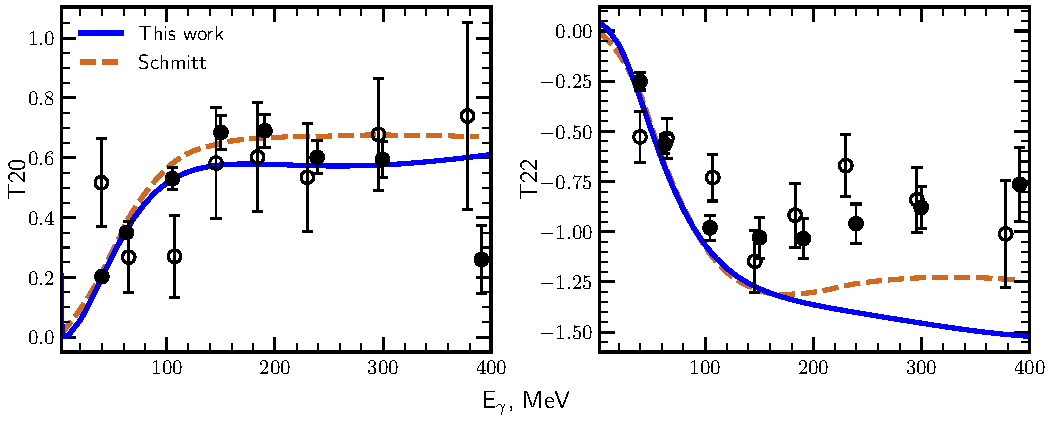
\includegraphics[width=0.9\textwidth]{Figures_De/T20_T22_vs_en.pdf}
        \end{center}
        \caption{
        The tensor analyzing powers T$_{20}$ (left) and T$_{22}$ (right) as
        a function of the photon energy E$_\gamma$
        at fixed outgoing proton angle $\theta_p = \ang{88}$ in the center of mass frame.
        My predictions (blue solid line) are obtained with the \gls{sms} potential at the chiral order \gls{n4lo+},
        with the cut-off parameter $\Lambda = \SI{450}{\mev}$ and with 2NC contributions included via the Siegert theorem.
        The dashed pink curve shows predictions obtained with the same interaction but without 2NC contributions.
        The dashed-dotted brown curve presents theoretical results from \cite{Schmitt1989}.
        Experimental data are taken from \cite{rachek2007} (filled circles)
        and \cite{mishev1993} (empty circles).}
        \label{T20_vs_en}
    \end{figure}

    \begin{figure}[h]
        \begin{center}
        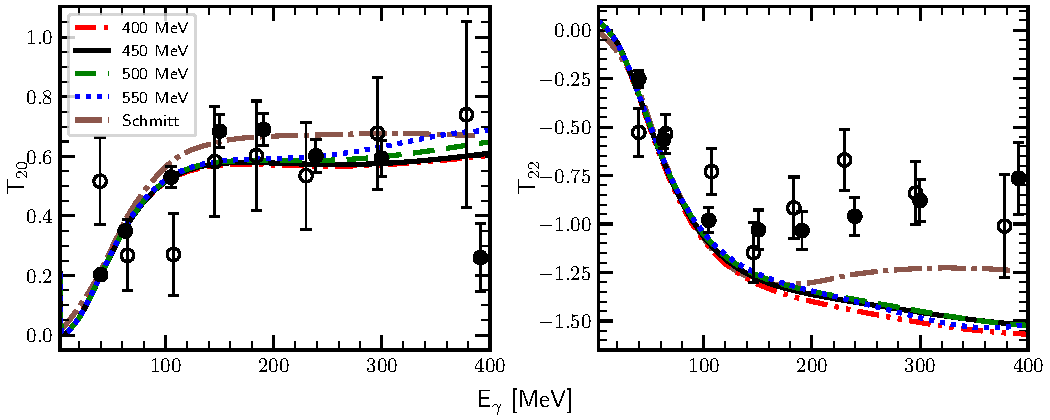
\includegraphics[width=0.9\textwidth]{Figures_De/T20_T22_vs_en_cutoff.pdf}
        \end{center}
        \caption{
        The tensor analyzing powers T$_{20}$ (left) and T$_{22}$ (right) as
        a function of the photon energy E$_\gamma$
        at fixed outgoing proton angle $\theta_p = \ang{88}$ in the center of mass frame.
        My predictions have been obtained with the \gls{sms} potential at the chiral order \gls{n4lo+},
        with the different values of the cut-off parameter $\Lambda$ (from \SI{400}{\mev} to \SI{550}{\mev}).
        The dashed-dotted brown curve presents theoretical results from \cite{Schmitt1989}.
        Experimental data are taken from \cite{rachek2007} (filled circles)
        and \cite{mishev1993} (empty circles).}
        \label{T20_vs_en_cutoff}
    \end{figure}

    \begin{figure}[h]
        \begin{center}
        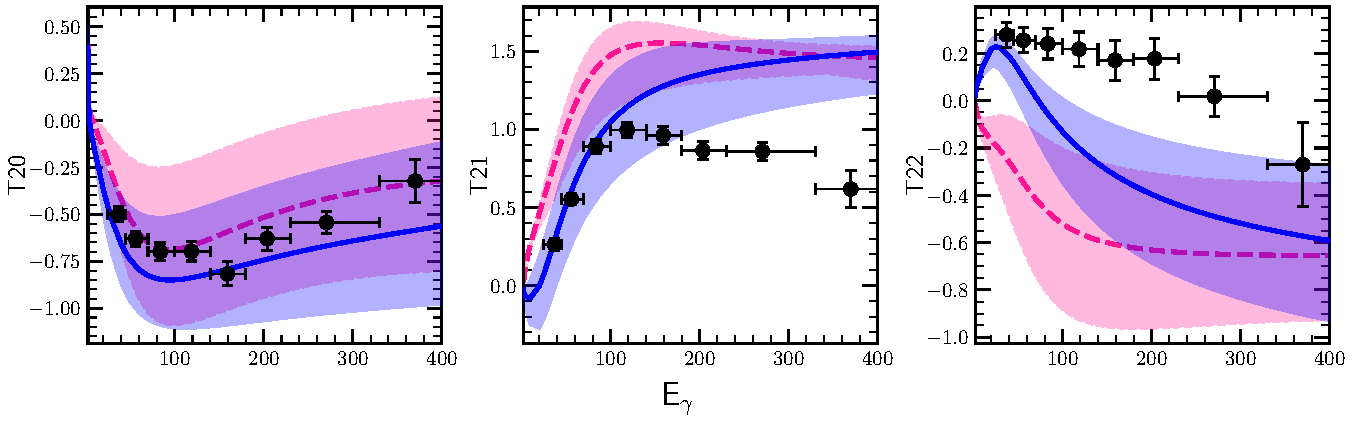
\includegraphics[width=0.95\textwidth]{Figures_De/TensorPower_Th24-48.pdf}
        \end{center}
        \caption{The averaged tensor analyzing powers T$_{20}$ (left),
        T$_{21}$ (middle) and T$_{22}$ (right) as a function of the
        photon energy for the outgoing proton momentum polar angle $\theta_p$
        in range $\ang{24} - \ang{48}$ in the center of mass frame.
        The solid blue curve is a mean value of my predictions at energy values ranges
        from 25 to \SI{45}{\mev}, obtained with
        the \gls{sms} potential at \gls{n4lo+} chiral order and with $\Lambda=\SI{450}{\mev}$
        and with \gls{snc} used together with the Siegert approach. 
        The pink dashed curve represents similar predictions but with
        the nuclear current reduced to the \gls{snc} only. 
        The corresponding bands show predictions at border energies 25 and \SI{45}{\mev}.
        The filled circles are experimental data
        from \cite{rachek2007} for the same energy range.}
        \label{tensor_energy_24-48}
    \end{figure}

    \begin{figure}[h]
        \begin{center}
        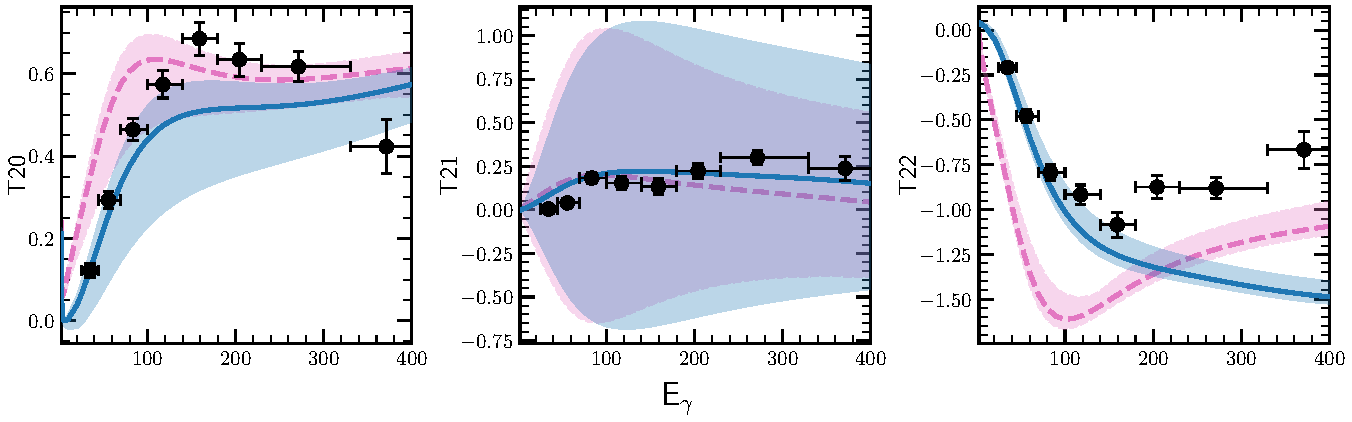
\includegraphics[width=0.95\textwidth]{Figures_De/TensorPower_Th70-102.pdf}
        \end{center}
        \caption{The same as in the \fig{tensor_energy_24-48} but
        for the $\theta_p$ in range $\ang{70} - \ang{102}$.}
        \label{tensor_energy_70-102}
    \end{figure}
    
    In the \fig{assymetry} I demonstrate predictions
    for the photon asymmetry $\Sigma_\gamma$ for the 
    deuteron photodisintegration with $\text{E}_\gamma=\SI{20}{\mev}$ (a)
    and \SI{60}{\mev}(b) together with the experimental data of 
    \cite{KRAUSE1992_asymetry, depascale_asymmetry, Barannik_asymetry, Vnukov_asymmetry}.
    Both (a) and (b) figures are organized similarly to the 
    figures I showed above for the tensor analyzing powers (e.g. \fig{T22_T11_30}).
    That is the top panel is aimed to demonstrate predictions obtained
    with the chiral \gls{sms} potential at different orders of the chiral expansion,
    the middle one shows a truncation error and the bottom one shows 
    the cut-off dependence. For that observable we see an excellent 
    convergence with respect to the chiral order. For both regarded 
    energies predictions at different orders are very close to each other
    except the \gls{lo} and \gls{nlo} curves. Nevertheless, at E$_\gamma = \SI{60}{\mev}$
    the truncation error bands reveal some uncertainty connected 
    with the chiral order and it is expected that even some higher chiral 
    orders would still contribute to the predictions at this energy.
    The relative width of the truncation band are 
    \SIlist{0.26;5.04;5.05;5.73;14.96}{\percent} for \gls{n4lo+}, \gls{n4lo}, \gls{n3lo},
    \gls{n2lo} and \gls{nlo} respectively and at $\theta_p=\ang{90}$.

    The cut-off dependence is also much stronger at \SI{60}{\mev}. One clearly sees
    that predictions are different for various values of the $\Lambda$.
    The relative difference between predictions to the cut-off parameter at \SI{20}{\mev}
    is \SI{0.26}{\percent} while at the photon energy \SI{60}{\mev}
    it is  \SI{4.41}{\percent} (both calculated at $\theta_p=\ang{90}$).
    So the theoretical uncertainty related to regulator value
    is nearly 17 times bigger than due to the truncation error ($4.11/0.26 = 16.96$).

     Comparing my predictions to experimental data, I observe that
     for the lower energy predictions are almost perfectly overlapping
     with experimental points within the error bars. 
     For a few data points our predictions are
     outside data error bars, but they are still within $3\sigma$ range.
     For \SI{60}{\mev}, experimental data points are systematically below theoretical
     curves, especially in the middle of the angular range. It seems that some systematic 
     uncertainty is presented in predictions and ad hoc multiplication by some factor
     (around 0.8)
     could help predictions be more similar to experimental data. But very likely the observed discrepancy
     points to the simplified character of the model used here.

     In the \fig{asymmetry_energy_1NC} the predictions obtained with the Full set of
     components (plane wave + rescattering and \gls{snc} + Siegert, solid blue curve) are shown
     versus predictions obtained without rescattering (green dashed-dotted line)
     and without contribution from the Siegert (pink dashed line) for the same 
     photon energies as above: E$_\gamma=\SI{20}{\mev}$ (left panel)
     and E$_\gamma=\SI{60}{\mev}$ (right panel).
     For the E$_\gamma=\SI{20}{\mev}$ the difference between Full and PW
     is quite small, whereas \gls{snc} is noticeably differs from the Full prediction,
     especially around the smallest and largest angle values.
     For the E$_\gamma=\SI{60}{\mev}$ the difference between such predictions 
     is larger: we see not only quantitative, but also qualitative variations.
     The \gls{snc} curve has much larger values and its shape becomes 
     more asymmetric with respect to the $\theta_p = \ang{90}$ point.

     In the \fig{asymmetry_90deg} (left) I present a dependence of the photon asymmetry
     $\Sigma_\gamma$ on the photon energy at a fixed value
     of the outgoing proton polar direction $\theta_p = \ang{90}$ 
     (following the data given at \cite{delbianco_1981} and \cite{depascale_asymmetry}).
     It is noticeable that with increasing energy, the predictions
     are systematically above the experimental data and the discrepancy growths with energy.
     This trend
     was also observed in the angular dependence of the asymmetry at \SI{60}{\mev}
     so I conclude that within our framework, 
     $\Sigma_\gamma$ is sensitive to the initial photon energy and some theoretical
     contributions are missing to get satisfactory predictions
     at higher energies. From the \fig{asymmetry_90deg} we can say that
     large discrepancy with data starts already above $\text{E}_\gamma = \SI{35}{\mev}$.
     \footnote{It is worth to note that data of \cite{depascale_asymmetry} are
     above these from \cite{delbianco_1981} (however still inside $3\sigma$ experimental
     error bands) and remain in agreement with my predictions even at E$_\gamma=\SI{60}{\mev}$.}

    The right panel of the \fig{asymmetry_90deg} shows an impact of the
    different model components to the obtained predictions.
    We see that the difference between the Full predictions (solid blue line)
    and the one obtained with a \gls{snc} only (without the Siegert contribution)
    is larger than the difference with predictions with plane-wave part only (without rescattering).
    Both these incomplete predictions are farther from the experimental data,
    (for PW at larger energies only) and have a different curve shape as well. 

    \begin{figure}[h]
        \centering
        \begin{subfigure}[b]{0.46\textwidth}
            \caption{\small E$_\gamma = \SI{20}{\mev}$}
            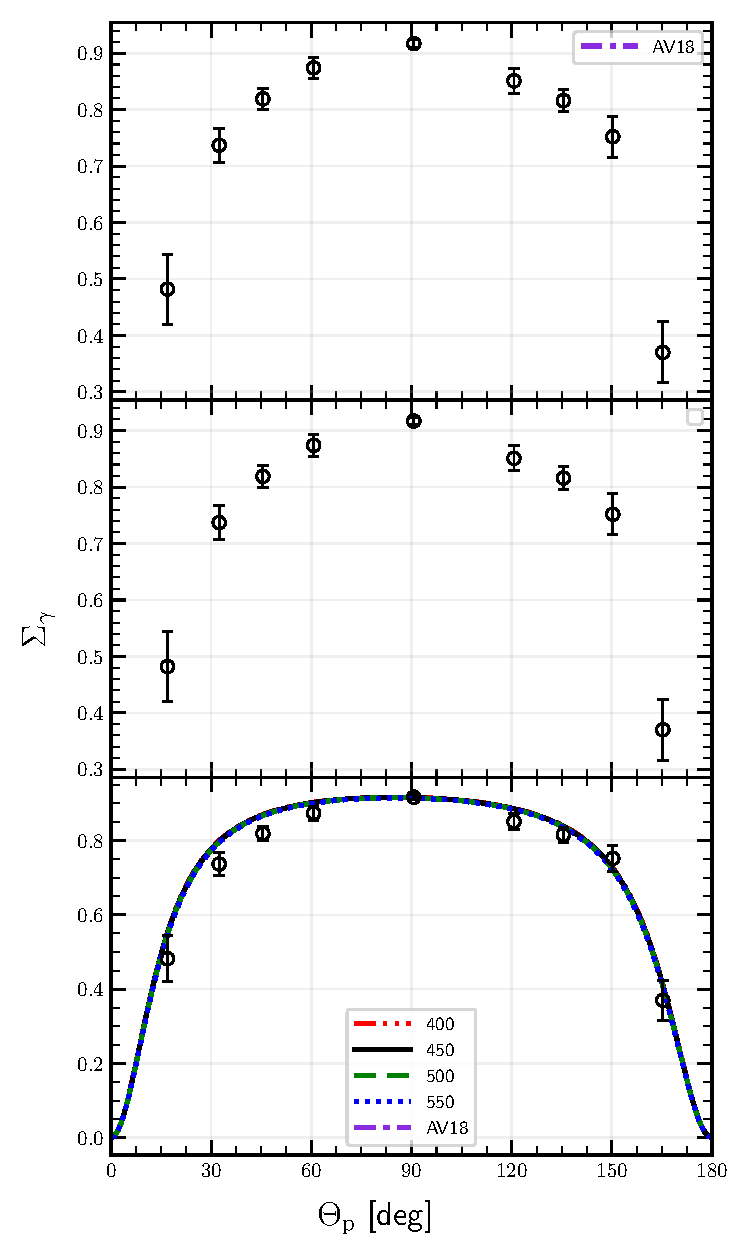
\includegraphics[width=\textwidth]{Figures_De/AX2_20mev.pdf}
            \label{AX_20_vert}
        \end{subfigure}
        \begin{subfigure}[b]{0.46\textwidth}
            \caption{\small E$_\gamma = \SI{60}{\mev}$}
            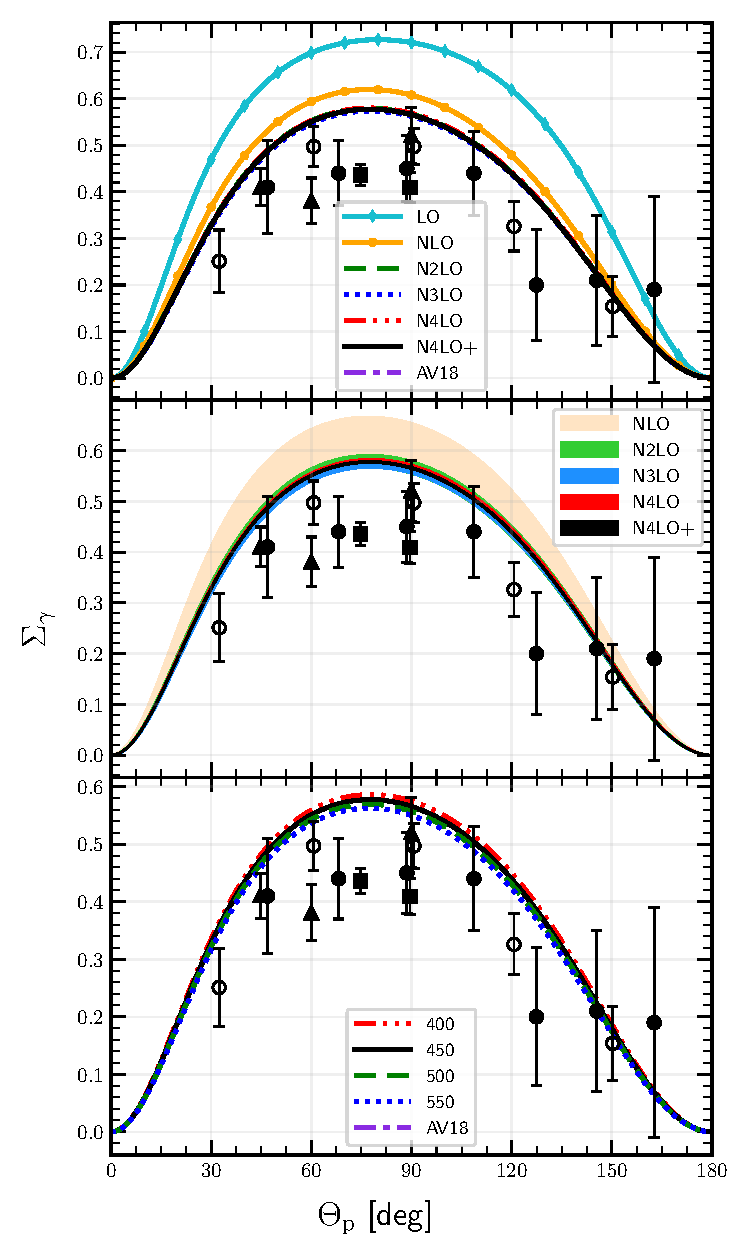
\includegraphics[width=\textwidth]{Figures_De/AX2_60mev.pdf}
            \label{AX_60_vert}
        \end{subfigure}
        \caption{The photon asymmetry $\Sigma_\gamma$ 
        as a function of the outgoing proton angle in the center of mass frame 
        for the photon energy \SI{20}{\mev}(a) and \SI{60}{\mev}(b).
        The top row presents results obtained using the \gls{sms} potential
        with chiral orders from \gls{lo} to \gls{n4lo+} and with the cut-off parameter $\Lambda=\SI{450}{\mev}$.
        The middle row shows truncation errors for each 
        chiral order starting from NLO and the
        bottom row presents a cut-off dependence for the chiral potential \gls{n4lo+}.
        Filled circles are experimental data from \cite{KRAUSE1992_asymetry},
        empty circles - from \cite{depascale_asymmetry}, filled squares
        - from \cite{Barannik_asymetry} and triangles are from \cite{Vnukov_asymmetry}.
        For the sake of comparison, predictions obtained with the \gls{av18} potential are
        given by the dashed-dotted curve as well.}
        \label{assymetry}
    \end{figure}


    \begin{figure}[h]
        \begin{center}
        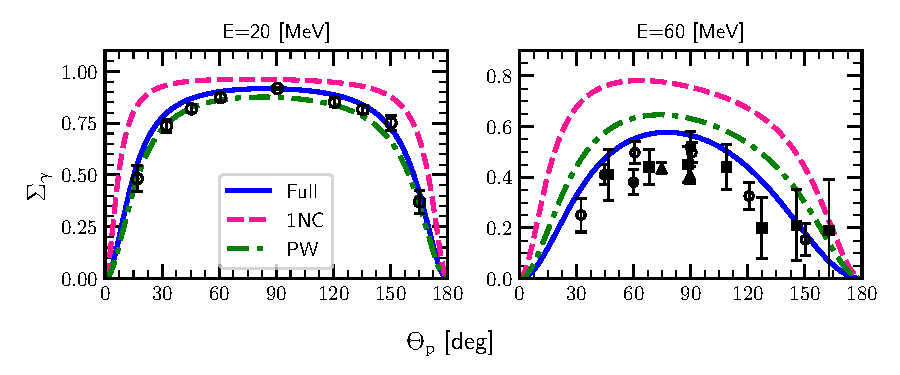
\includegraphics[width=0.95\textwidth]{Figures_De/Asymetry_20-60mev_pw_1nc.pdf}
        \end{center}
        \caption{The photon asymmetry $\Sigma_\gamma$ as a function of the
        outgoing proton angle $\theta_p$ in the \gls{cm} frame at $\text{E}_\gamma = \SI{20}{\mev}$
        (left) and $\text{E}_\gamma = \SI{60}{\mev}$(right).
        Similarly to \fig{Diff_cross_pw_1nc} predictions obtained with chiral \gls{n4lo+} potential
        and $\Lambda=\SI{450}{\mev}$ are presented for three theoretical models.
        The blue solid line is the most complete prediction we have (plane-wave plus rescattering parts, 1NC + Siegert), the pink dashed line shows predictions obtained with
        single-nucleon current only (1NC) - without the Siegert contributions and the green dashed-dotted line
        is a prediction in which we neglect the rescattering part
        and stick to the plane-wave part only but keeping the Siegert contributions.
        Filled circles are experimental data from \cite{KRAUSE1992_asymetry},
        empty circles - from \cite{depascale_asymmetry}, filled squares
        - from \cite{Barannik_asymetry} and triangles are from \cite{Vnukov_asymmetry}.}
        \label{asymmetry_energy_1NC}
    \end{figure}

     
    \begin{figure}[h]
        \begin{center}
        % 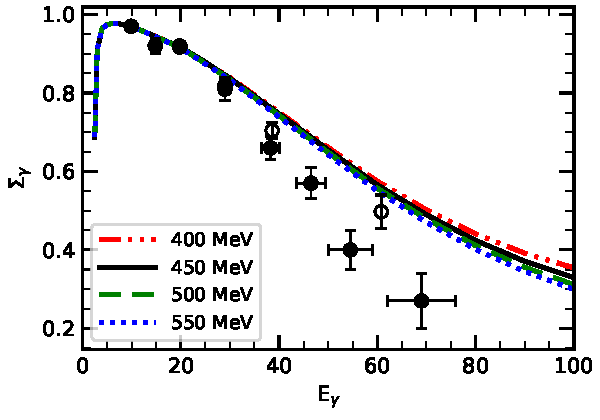
\includegraphics[width=0.75\textwidth]{Figures_De/AX2_90deg.pdf}
        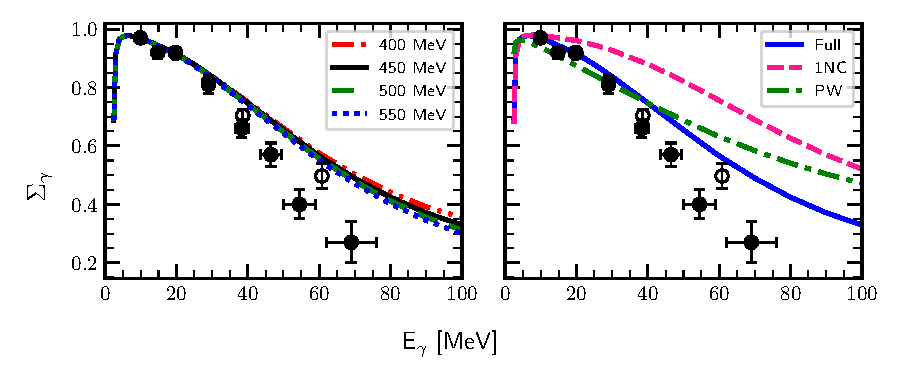
\includegraphics[width=0.95\textwidth]{Figures_De/AX2_90deg_1NC_PW.pdf}
        \end{center}
        \caption{The photon asymmetry $\Sigma_\gamma$ 
        as a function of the photon energy  
        at the fixed outgoing proton's momentum polar angle $\theta_p=90^\circ$.
        On the left panel, each curve corresponds to the particular value of the cut-off parameter
        and chiral potential used here is the \gls{n4lo+} one.
        On the right panel, the blue solid curve represents our most complete predictions
        comprising the plane-wave plus rescattering parts and \gls{snc}+Siegert current propagator 
        (the same as \SI{450}{\mev} line in left).
        The pink dashed curve shows predictions obtained with
        the single-nucleon current only (without applying the Siegert theorem) and the green dashed-dotted
        curve represents predictions with the full current (\gls{snc} + Siegert) but plane-wave part only.
        Filled circles are experimental data from \cite{delbianco_1981},
        empty circles - from \cite{depascale_asymmetry}.}
        \label{asymmetry_90deg}
    \end{figure}


    The proton polarization is demonstrated in \fig{PY_30_100_vert} for the 
    photon energy \SI{30}{\mev}(a) and \SI{100}{\mev}(b).
    In this case even at higher energy
    (such as \SI{100}{\mev}) predictions reveal neither slower convergence concerning the chiral order nor stronger cut-off dependence. Figures for both energies show
    that only next-to-leading order brings a relatively high contribution
    while taking into account other subsequent orders does not change predictions
    significantly. In the case of the cut-off dependence, we see that curves for each
    value of $\Lambda$ are very close to each other. 
    The relative difference of the predictions with respect to the cut-off parameter
    is \SI{4.04}{\percent} at the minimum point $\theta_p=\ang{130}$ of $\text{E}_\gamma = \SI{30}{\mev}$
    and \SI{5.62}{\percent} at $\theta_p=\ang{160}$ and $\text{E}_\gamma = \SI{100}{\mev}$.
    The dependence is slightly stronger for higher energy, but both values are comparable.
    Again, the cut-off-related uncertainty exceeds the truncation error.

    \begin{figure}[h]
        \centering
        \begin{subfigure}[b]{0.46\textwidth}
            \caption{\small E$_\gamma = 30$~MeV}
            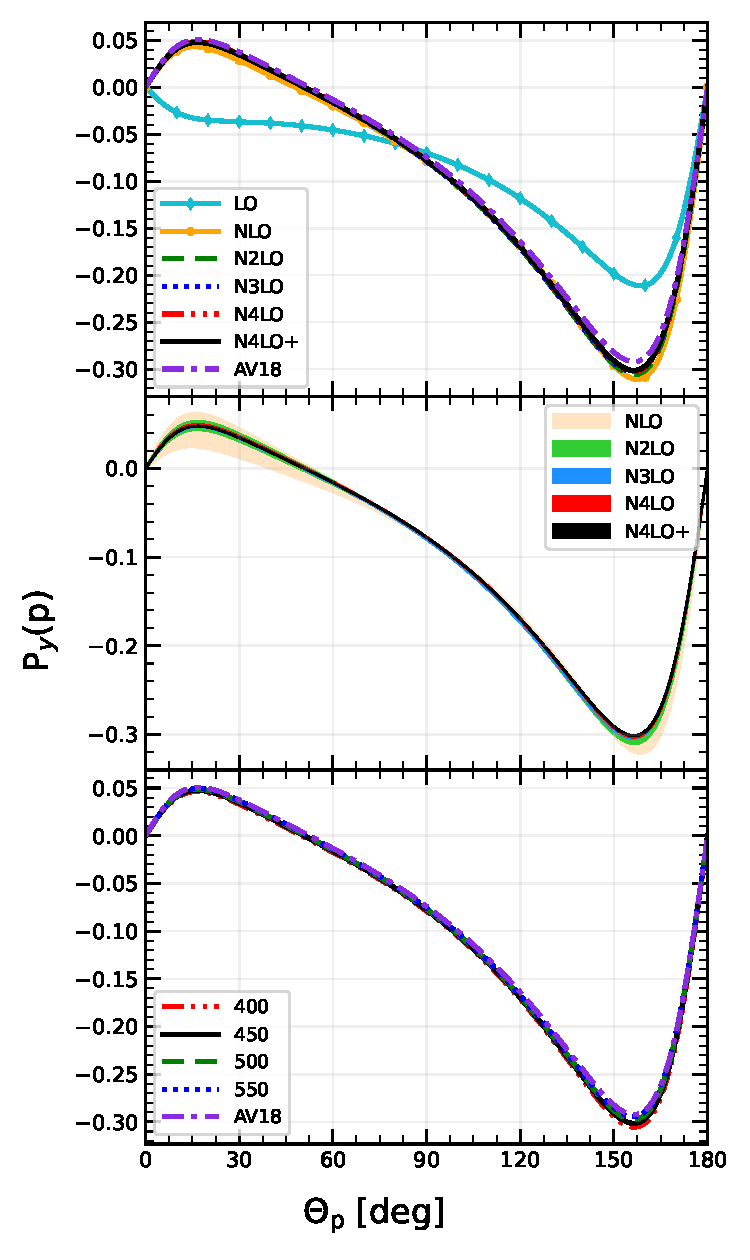
\includegraphics[width=\textwidth]{Figures_De/POLNOUT2(y)_30mev.pdf}
            \label{PY_30_vert}
        \end{subfigure}
        \begin{subfigure}[b]{0.46\textwidth}
            \caption{\small E$_\gamma = 100$~MeV}
            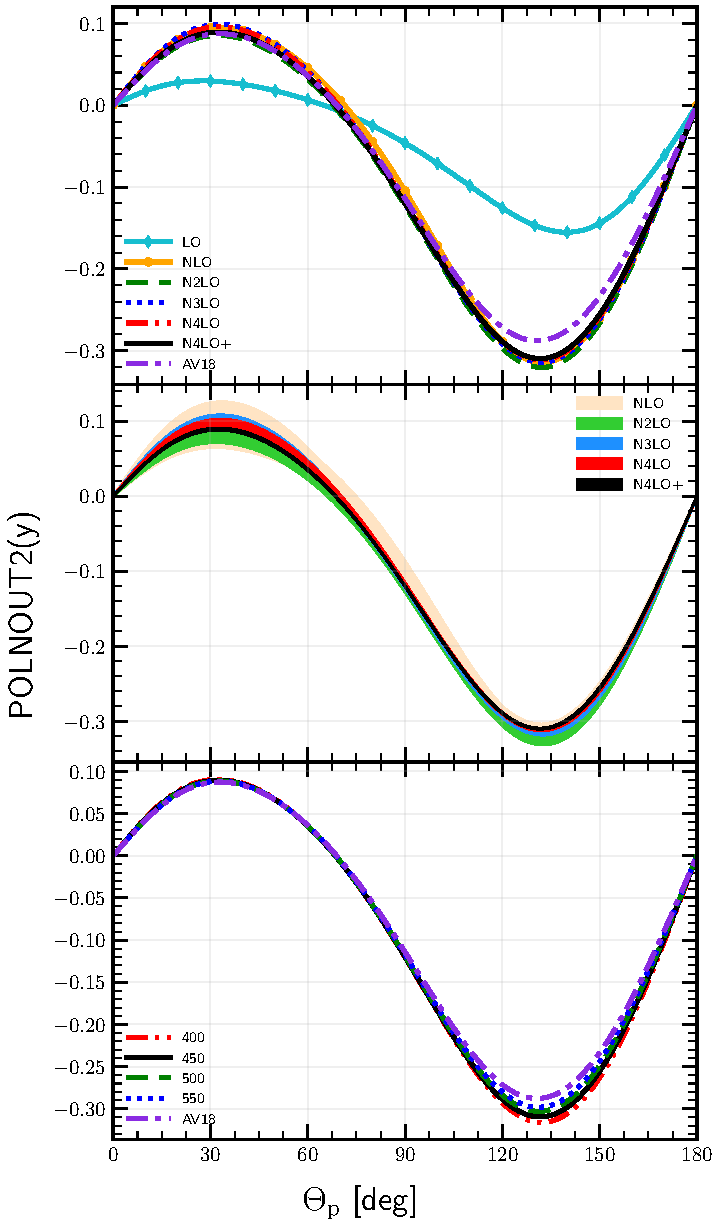
\includegraphics[width=\textwidth]{Figures_De/POLNOUT2(y)_100mev.pdf}
            \label{PY_100_vert}
        \end{subfigure}
        \caption{Proton polarization $P_y(p)$ 
        \label{PY_30_100_vert}
        as a function of the outgoing proton's momentum polar angle in the center of mass frame 
        with the photon energy \SI{30}{\mev} (a) and \SI{100}{\mev} (b).
        The top figures present results obtained using potential
        with different chiral orders (from \gls{lo} to \gls{n4lo+}) with cut-off parameter $\Lambda=\SI{450}{\mev}$.
        The middle panel shows truncation errors for each 
        chiral order starting from \gls{nlo} and
        bottom figures present a cut-off dependence of predictions
        based on the \gls{sms} \gls{n4lo+} potential.
        For the sake of comparison, predictions obtained with the \gls*{av18} potential 
        are shown as well.}
    \end{figure}



    Predictions for the neutron polarization at the energies \SI{2.75}{\mev} and \SI{100}{\mev} are shown in the
    \fig{Pn_2p75_100}. The choice of energy is conditioned by the availability of experimental data,
    which were taken in 1965 in Livermore \cite{Jewell_neuteronpolarization} and 
    in 1986 at TRIUMF facility \cite{CAMERON_neuteronpolarization}.
    In the case of E$_\gamma = \SI{2.75}{\mev}$ (\fig{Pn_2p75_vert}), we see that predictions reflect
    the behavior of experimental data points qualitatively,
    having more o less a constant offset of the values. A similar offset was obtained
    also in \cite{ArenhovelPhotodisint1991}, where various approaches were presented.
    Authors compare different models which leads to very similar theoretical results
    even though different potentials are used with and without relativistic correction.
    One of the theoretical predictions is included even in the experimental papers
    \cite{Jewell_neuteronpolarization} and authors state that there might be a
    systematic error in the calibration of the analyzing power
    of the neutron polarimeter which could affect experimental results precision.
    Interestingly, predictions clearly show a symmetrical form of the curve, while the experimental data
    have some deviations from the symmetrical form. It can be a sign that some problem with the data can be
    in this case (taking into account also that the experiment had been done in 1965).
    In \cite{Jewell_neuteronpolarization} authors even make a plot of the theoretical curve
    multiplied by the factor 0.879 which almost perfectly overlaps with experimental data afterward. 

    At the energy E$_\gamma = \SI{100}{\mev}$ (\fig{Pn_100_vert}) 
    my predictions describe the data very well.
    For most of the data points, predicted values are within error bars, and only some
    of the points (e.g. around \ang{50}) have a prediction in distance more than one standard deviation.
    Nevertheless, these data points look like they are out of general trend and may be
    a result of imprecise measurement.
    Observing the stability of my predictions on the chiral order and regulator value I 
    conclude that nucleon polarizations are not the observables, which, even measured with much
    better precision, than it was done in \cite{Jewell_neuteronpolarization} or \cite{CAMERON_neuteronpolarization}
    would be an indicator of the model convergence or stability.

    Concluding my results of the deuteron photodisintegration predictions, 
    I can point that predictions for $\text{E}_\gamma = \SI{30}{\mev}$ (and lower)
    are very stable with respect to the potential parameters (chiral order or the regulator).
    It shows an ability for a good data description as well. For a higher energies (especially above \SI{100}{\mev})
    the quality of predictions becomes lower: the dependency on the cut-off value is higher as well as 
    discrepancy with experimental data. Still, predictions are converged with respect to the chiral order.
    The general problem is a lack of 2N current and in the case of higher energies - relativistic corrections are missing. 


    \begin{figure}[h]
        % \centering
        % 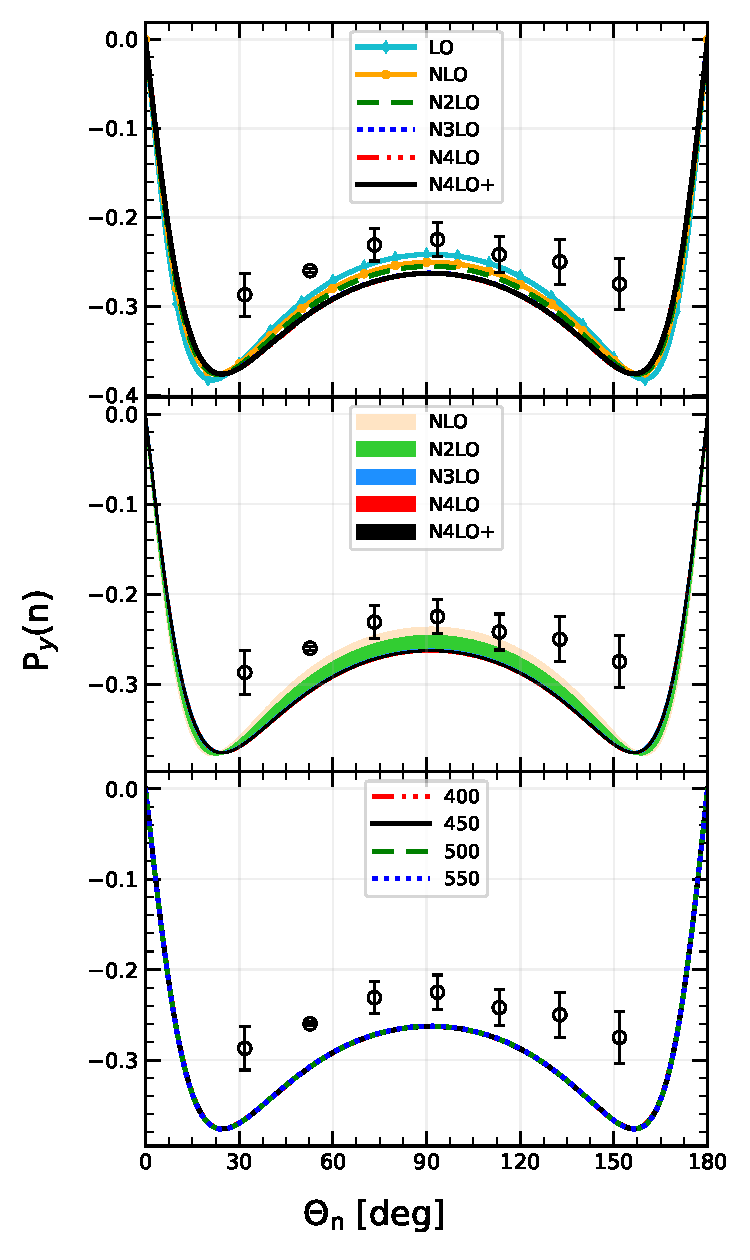
\includegraphics[width=0.5\textwidth]{Figures_De/POLNOUT2(y)_2.75mev_neuteron.pdf}
        \centering
        \begin{subfigure}[b]{0.46\textwidth}
            \caption{\small E$_\gamma = 2.75$~MeV}
            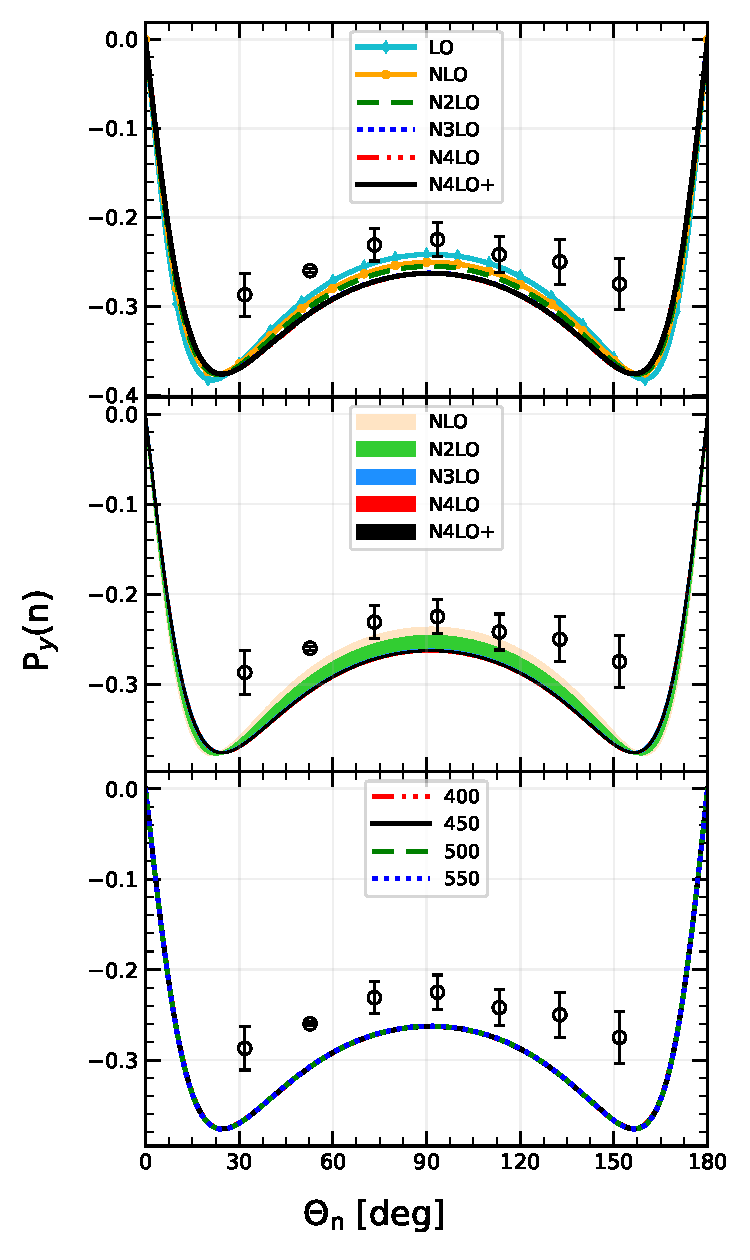
\includegraphics[width=\textwidth]{Figures_De/POLNOUT2(y)_2.75mev_neuteron.pdf}
            \label{Pn_2p75_vert}
        \end{subfigure}
        \begin{subfigure}[b]{0.46\textwidth}
            \caption{\small E$_\gamma = 100$~MeV}
            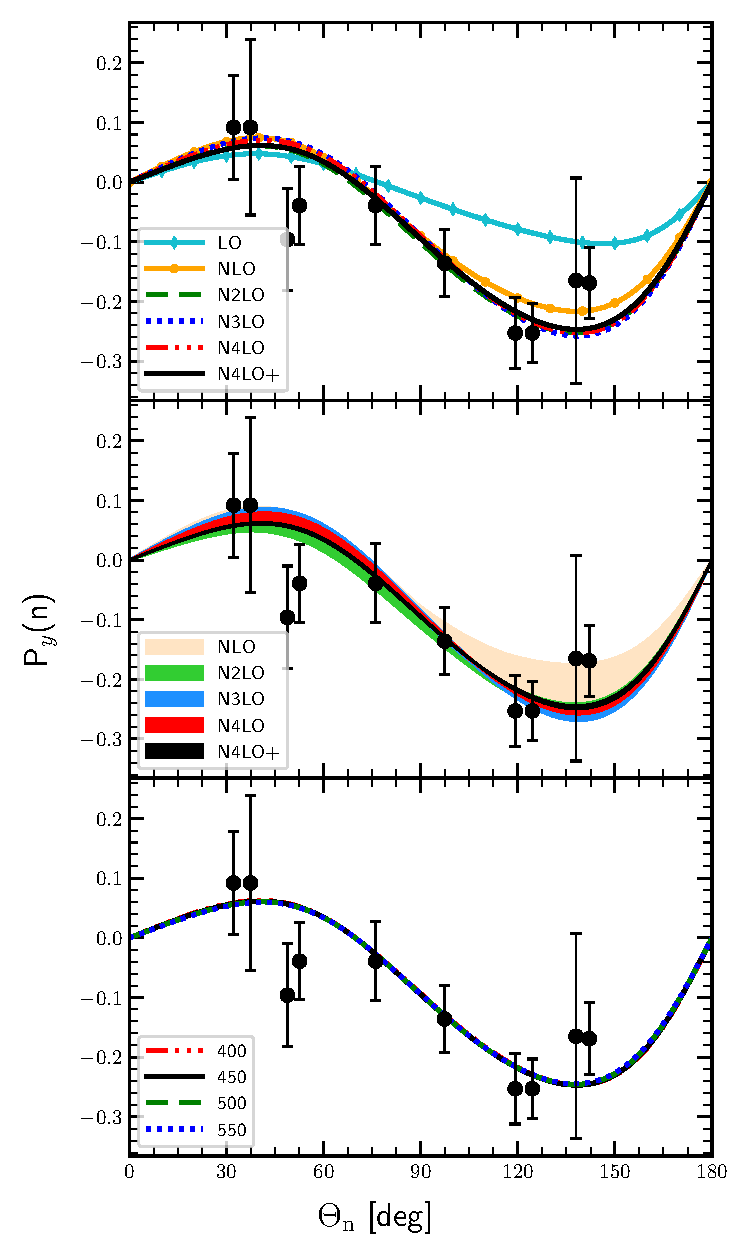
\includegraphics[width=\textwidth]{Figures_De/POLNOUT2(y)_100mev_neuteron.pdf}
            \label{Pn_100_vert}
        \end{subfigure}
        \caption{The same as in \fig{PY_30_100_vert} but for the neutron polarization
        $P_y(n)$ and at photon energies \SI{2.75}{\mev} {\bf (a)} and \SI{100}{\mev} {\bf (b)}.
        Data are from \cite{Jewell_neuteronpolarization} (empty circles)
        and \cite{CAMERON_neuteronpolarization} (filled circles).}
        \label{Pn_2p75_100}
    \end{figure}


\clearpage

\section{Helium-3 photodisintegration}
\label{sec:hel_results}

\subsection{Three-body breakup}
\label{sec:hel_3N}

    In this section I will discuss results
    for $^3\text{He} \rightarrow p + p + n$ differential
    cross-section obtained with the \gls{snc} + Siegert model of nuclear current.
    For three free nucleons in the final state, it is convenient to
    introduce, as a kinematical variable, the arc-length of the S-curve.
    For a given direction of two momenta $\hat{p}_1$ and $\hat{p}_2$,
    the S-curve spans in the plane defined by kinetic energies of the 
    same two nucleons, $E_1$ and $E_2$.

    For three particles and known initial energy and momenta five kinematical
    variables\footnote{Among nine variables describing final state 
    $\vec{p}_1,\vec{p}_2$ and $\vec{p}_3$, four can be derived from 
    energy and momentum conservation laws.}
    are required to define the final kinematics.
    We choose four variables as directions of outgoing nucleons no 1 and 2:
    $\theta_1, \phi_1, \theta_2$ and $\phi_2$, with the $z$-axis aligned to the 
    photon momentum. Choosing $E_1$ as the fifth variable would introduce
    ambiguity, as in some cases two values of $E_2$ could be allowed.
    Instead, the location on the S-curve defines the kinematical configuration
    unambiguously.
    The various possible locations of the S-curve in $E_1-E_2$ plane,
    as well as the convention on choosing the $S=0$ point is given
    in Fig.~1 of \cite{GLOCKLE_report_1996}.
    
    In the \fig{CROSS_HE_EXCL_30} I demonstrate a differential cross section 
    $\frac{d^5\sigma}{d\Omega_1d\Omega_2dS}$ as a function of the S arc length
    and as in the previous section, I study the convergence with respect to chiral
    order and the cut-off dependence.
    The photon energy is  E$_\gamma=\SI{30}{\mev}$; the kinematic configuration
    $\theta_1 = \ang{15}$, $\phi_1 = \ang{0}$,
    $\theta_2 = \ang{15}$, $\phi_2 = \ang{180}$ and predictions have been
    obtained without 3NF.\footnote{Different kinematic configurations $\theta_1$, $\phi_1$,
    $\theta_2$ and $\phi_2$ have been tested with a step of \ang{15}
    and most interesting cases(showing the largest discrepancies) are presented in this work.}
    On the left, we see that only \gls{nlo} and \gls{n2lo} introduce relatively large truncation errors.
    The maximal width of a band for NLO is \SI{37.6}{\percent} at $S=\SI{10}{\mev}$,
    for \gls{n2lo} it is \SI{12.4}{\percent} at the same S-value and it is gradually decreasing
    coming to \SI{0.13}{\percent} at \gls{n4lo+}.
    The cut-off spread(right) is bigger around maxima values but remains below
    \SI{3}{\percent}. It reaches
    \SI{0.78}{\percent} at the minimum point ($S=\SI{10}{\mev}$).
    

    \begin{figure}[h]
        \begin{center}
            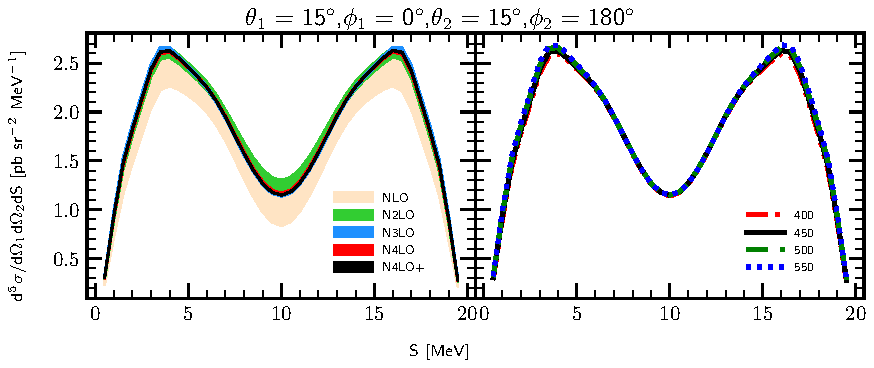
\includegraphics[width=0.9\textwidth]{Figures_HE/CROSS_excl_trunc_30mev.pdf}
            \end{center}
            \caption{The five-fold differential cross section for the photon 
            energy E$_\gamma=\SI{30}{\mev}$ for the kinematic configuration
            $\theta_1 = \ang{15}$, $\phi_1 = \ang{0}$,
            $\theta_2 = \ang{15}$, $\phi_2 = \ang{180}$.
            The left figure presents truncation error bands obtained using the \gls{sms} potential
            with chiral orders from \gls{nlo} to \gls{n4lo+}, and with
            cut-off parameter $\Lambda=\SI{450}{\mev}$.
            The right figure presents a cut-off dependence at \gls{n4lo+}.
            Results are obtained with two-nucleon force only and \gls{snc} current
            and Siegert theorem used for 2NC contributions.}
            \label{CROSS_HE_EXCL_30}
        \end{figure}

    With larger energy E$_\gamma=\SI{100}{\mev}$, for which predictions
    are demonstrated in the \fig{CROSS_HE_EXCL_100},
    both truncation error and cut-off spread become larger.
    The truncation band at the maximum point at $S=\SI{10}{\mev}$ for NLO is \SI{55.0}{\percent}
    decreasing to \SI{2.2}{\percent} at \gls{n4lo+} which still is around 3 times larger than
    it was for predictions at E$_\gamma=\SI{30}{\mev}$.
    The cut-off spread also becomes larger with increasing energy value: \SI{9.0}{\percent}
    at the same (maximum) point which is also $\sim 3$ times bigger than the one we observed
    for the lower energy.

        \begin{figure}[h]
            \begin{center}
            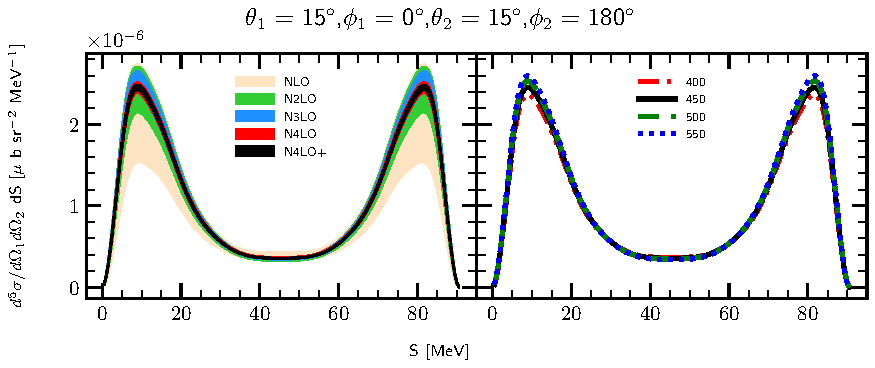
\includegraphics[width=0.9\textwidth]{Figures_HE/CROSS_excl_trunc_100mev.pdf}
            \end{center}
            \caption{The same as in \fig{CROSS_HE_EXCL_30} but 
            for the photon energy E$_\gamma=100$~MeV}
            \label{CROSS_HE_EXCL_100}
        \end{figure}

    Results for the same E$_\gamma=100$~MeV but other angular configuration  
    $\theta_1 = \ang{75}$, $\phi_1 = \ang{75}$,
    $\theta_2 = \ang{75}$, $\phi_2 = \ang{105}$ are
    given in \fig{CROSS_HE_EXCL_75_75_75_105}.
    The top row shows results obtained with 2NF only, while predictions obtained with 3NF are shown
    on the bottom row.
    It seems that 3NF does not change much the convergence with respect to the chiral order:
    truncation error band at the point of maximum $S=\SI{35}{\mev}$ (\gls{n4lo+})
    is \SI{1.11}{\percent} and \SI{1.16}{\percent} with and without 3NF, respectively.
    As it is almost the same, I conclude that inclusion \gls{n2lo} 3NF practically
    does not affect chiral order convergence.
    Note, 3NF at \gls{n2lo} has been used for all forces above \gls{nlo}.

    The cut-off dependence, in turn, is affected by the presence of 3NF. Predictions with 2NF only have
    \SI{13.7}{\percent} spread at the same maximum point $S=\SI{35}{\mev}$, while predictions with 3NF
    have only \SI{1.23}{\percent} relative spread, so the difference is tremendous.

        \begin{figure}[h]
            \begin{center}
                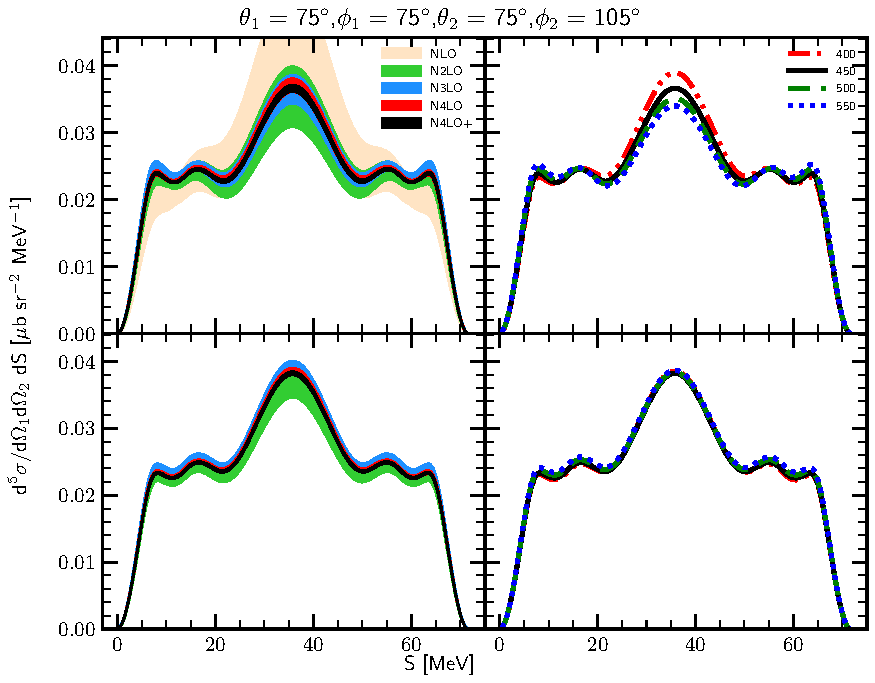
\includegraphics[width=0.9\textwidth]{Figures_HE/CROSS_excl_trunc_100mev_75_75_75_105_2NF_3NF.pdf}
                \end{center}
                \caption{The same as in the \fig{CROSS_HE_EXCL_100} but for the kinematic
                configuration at
                $\theta_1 = \ang{75}$, $\phi_1 = \ang{75}$,
                $\theta_2 = \ang{75}$ and $\phi_2 = \ang{105}$.
                Results obtained with the chiral \gls{sms} 2N force 
                are presented on the top row. The same, but
                with the \gls{n2lo} 3NF included is presented on the bottom row
                (starting from the \gls{n2lo} - where 3NF appears for the first time).}
                \label{CROSS_HE_EXCL_75_75_75_105}
        \end{figure}


    Similar trends are present also in other configurations, demonstrated for the comparison:
    Figs.\ref{CROSS_HE_EXCL_15_105_15_75},
    Figs.\ref{CROSS_HE_EXCL_45_75_45_105} and
    Figs.\ref{CROSS_HE_EXCL_165_15_15_165}.

    
        \begin{figure}[h]
            \begin{center}
                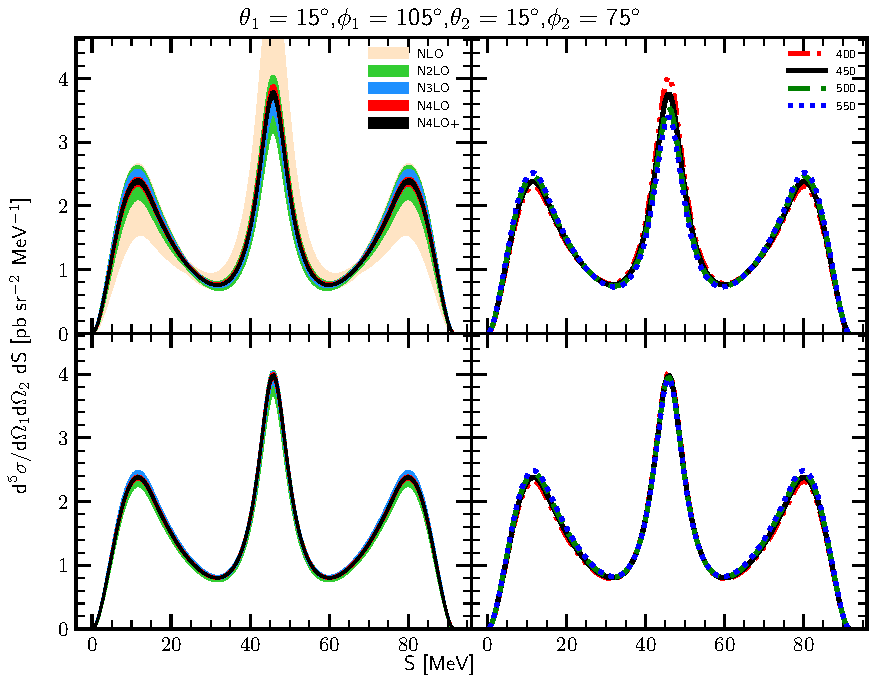
\includegraphics[width=0.9\textwidth]{Figures_HE/CROSS_excl_trunc_100mev_15_105_15_75_2NF_3NF.pdf}
                \end{center}
                \caption{The same as in the \fig{CROSS_HE_EXCL_75_75_75_105} but for the kinematic
                configuration at
                $\theta_1 = \ang{15}$, $\phi_1 = \ang{105}$,
                $\theta_2 = \ang{15}$ and $\phi_2 = \ang{75}$.}
                \label{CROSS_HE_EXCL_15_105_15_75}
        \end{figure}




        \begin{figure}[h]
            \begin{center}
                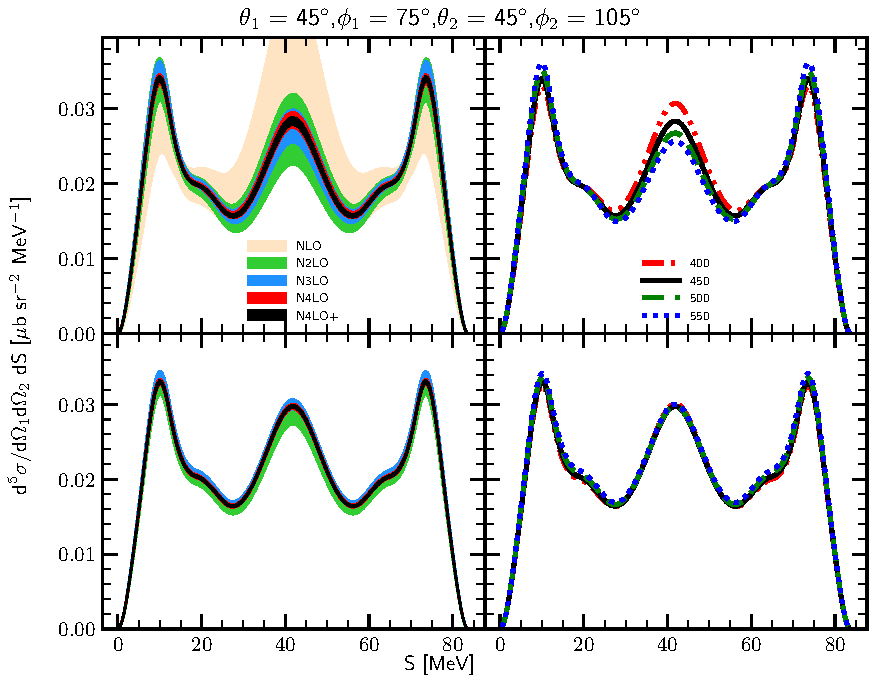
\includegraphics[width=0.9\textwidth]{Figures_HE/CROSS_excl_trunc_100mev_45_75_45_105_2NF_3NF.pdf}
                \end{center}
                \caption{The same as in the \fig{CROSS_HE_EXCL_15_105_15_75} but for the different kinematic
                configuration.}
                \label{CROSS_HE_EXCL_45_75_45_105}
        \end{figure}


        \begin{figure}[h]
            \begin{center}
                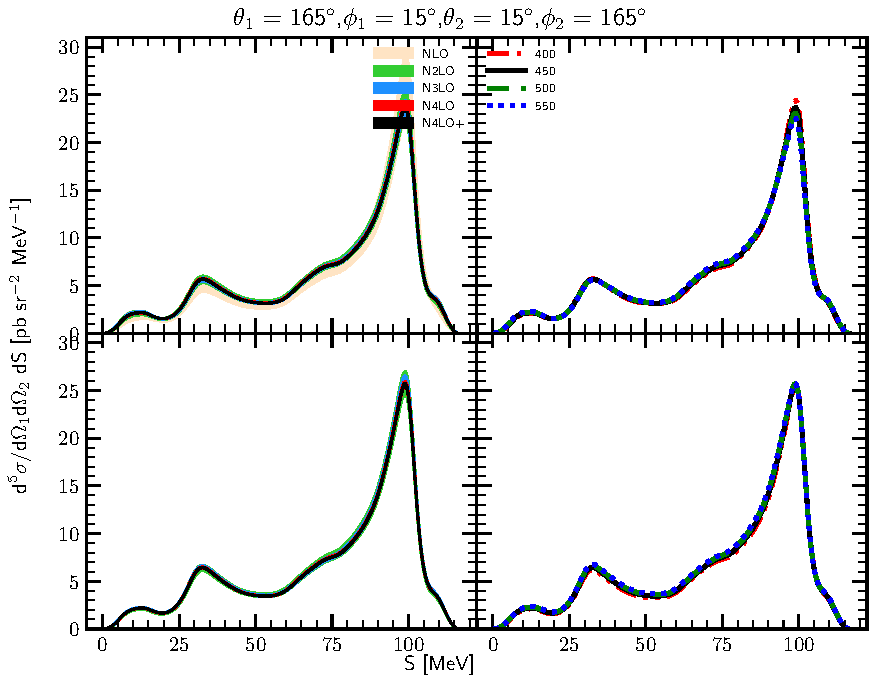
\includegraphics[width=0.9\textwidth]{Figures_HE/CROSS_excl_trunc_100mev_165_15_15_165_2NF_3NF.pdf}
                \end{center}
                \caption{The same as in the \fig{CROSS_HE_EXCL_45_75_45_105} but for the kinematic
                configuration at
                $\theta_1 = \ang{165}$, $\phi_1 = \ang{15}$,
                $\theta_2 = \ang{15}$ and $\phi_2 = \ang{165}$.}
                \label{CROSS_HE_EXCL_165_15_15_165}
        \end{figure}


        The exclusive cross-sections shown above, in Figs.~\ref{CROSS_HE_EXCL_30}-\ref{CROSS_HE_EXCL_165_15_15_165}
        are small and unfortunately below the possibilities of current 
        experimental techniques. The semi-inclusive measurement is more likely to be
        performed, thus in Figs \ref{CROSS_HE_INCL_30MEV_2NF} and \ref{CROSS_HE_INCL_100MEV_2NF}
        I show the 
        differential cross section $\frac{d^3\sigma}{d\Omega_p d\text{E}_p}$.
        I choose the same photon energies as above: E$_\gamma = \SI{30}{\mev}$ and
        E$_\gamma = \SI{100}{\mev}$.
        Each figure consists of subfigures where each row presents results
        for a proton momenta polar angle $\theta_p = \ang{10}, \ang{50}, \ang{90}, \ang{130}$ and \ang{170}.
        The left part of each subfigure shows detected
        chiral order dependence while the right - the cut-off dependence.
        
        At the photon energy \SI{30}{\mev} the chiral dependence is relatively weak: at the maximum point
        ($E_p \simeq \SI{3.8}{\mev}$) the relative difference varies between \SI{12}{\percent} and 
        \SI{28}{\percent} at LO for different angles. This difference decreases with each subsequent order
        resulting in maximum \SI{0.15}{\percent} at $N^4LO+$. At the energy $\text{E}_\gamma = \SI{100}{\mev}$ truncation errors
        are larger: at the maximum around $E_p \simeq \SI{1.46}{\mev}$ the discrepancy is around \SI{40}{\percent} (NLO),
        \SI{15}{\percent} (N2LO), coming to \SI{1.5}{\percent} at \gls{n4lo+}.

        A typical cut-off uncertainty at $\text{E}_\gamma = \SI{30}{\mev}$ is around \SI{2}{\percent}
        and at $\text{E}_\gamma = \SI{100}{\mev}$ increases up to \SI{8}{\percent} for all angles and 
        at the same values of $E_p$ as regarded above.

        Observed small uncertainties allow me to conclude that the semi-inclusive cross-section
        $\frac{d^3\sigma}{d\Omega_p d\text{E}_p}$ is not useful in studies aiming on
        pin-down the details of the chiral force.
        \tmp{do we have prediction with other current ::: calculate with ISIEGERT=0, IMEC=0 and compare results 
        for one configuration for 30 MeV and for 100 MeV}  



        \begin{figure}[h]
            \begin{center}
            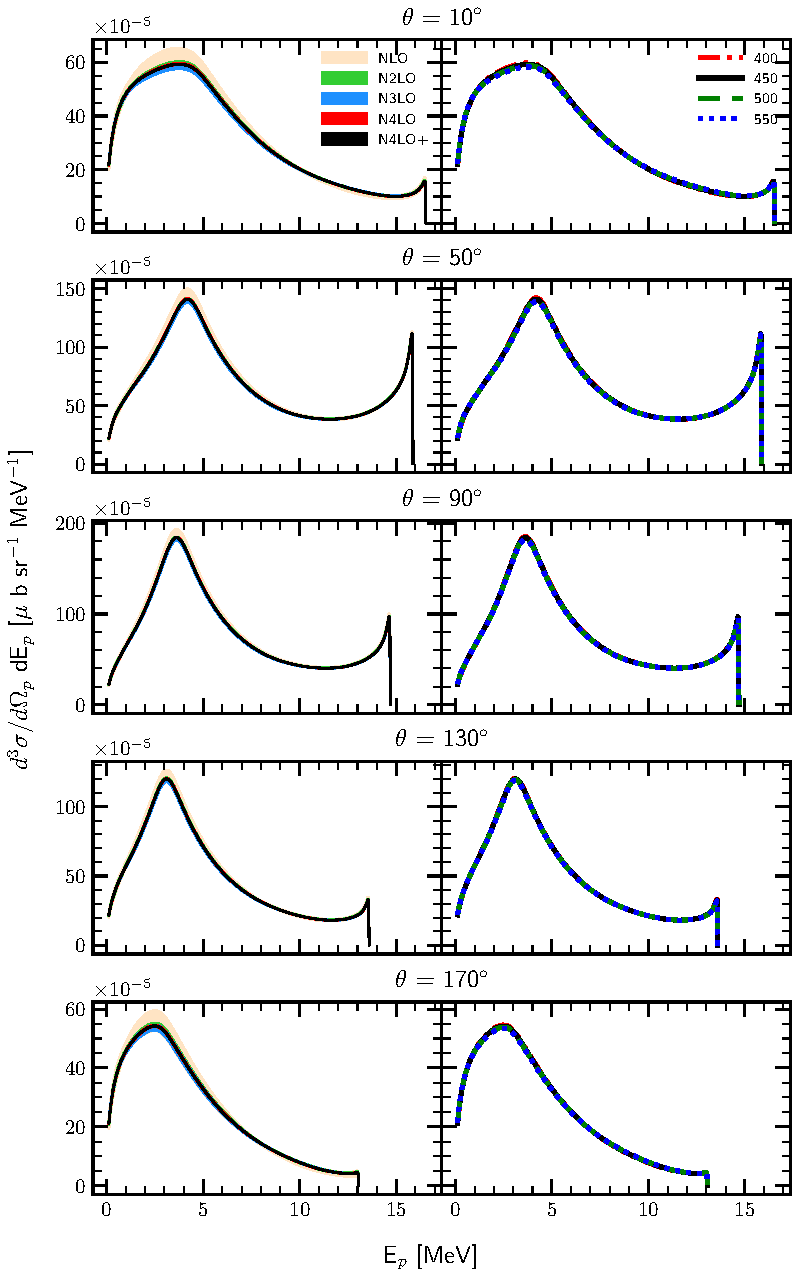
\includegraphics[width=0.8\textwidth]{Figures_HE/CROSS_incl_trunc_30mev_all.pdf}
            \end{center}
            \caption{The semi-inclusive differential cross section $\frac{d^3\sigma}{d\Omega_p d\text{E}_p}$
            at E$_\gamma = \SI{30}{\mev}$ $\phi_1 = \ang{0}$ as a function of outgoing proton energy E$_p$. Each row represents 
            predictions for different values of the outgoing proton's momentum polar angle $\theta_p$: 
            \ang{10}, \ang{50}, \ang{90}, \ang{130} and \ang{170}.
            The left figure presents truncation error bands obtained using the \gls{sms} potential
            with chiral orders from \gls{nlo} to \gls{n4lo+}, and with
            cut-off parameter $\Lambda=\SI{450}{\mev}$.
            The right figure presents a cut-off dependence at \gls{n4lo+}.
            Predictions have been obtained with the \gls{sms} NN potential but neglecting 3NF.}
            \label{CROSS_HE_INCL_30MEV_2NF}
        \end{figure}

        \begin{figure}[h]
            \begin{center}
            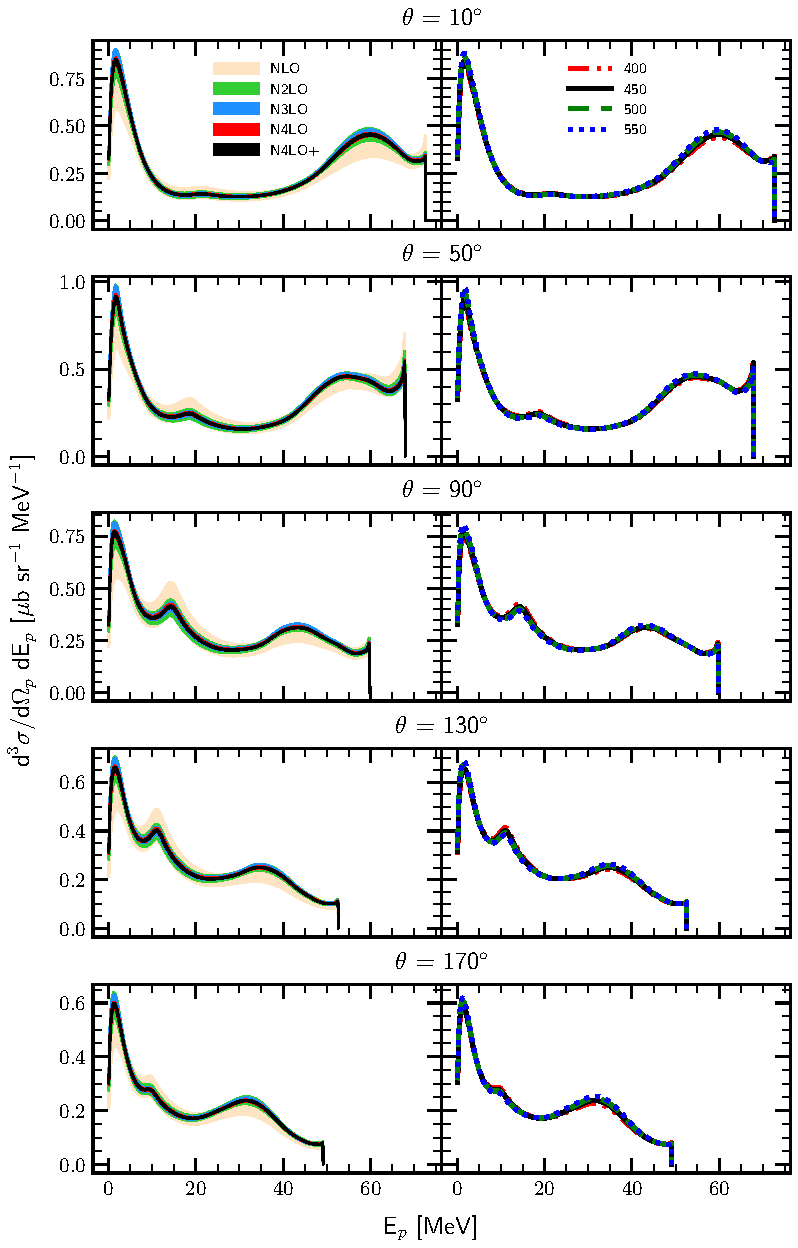
\includegraphics[width=0.8\textwidth]{Figures_HE/CROSS_incl_trunc_100mev_all.pdf}
            \end{center}
            \caption{The same as in \fig{CROSS_HE_INCL_30MEV_2NF} but for E$_\gamma = \SI{100}{\mev}$.}
            \label{CROSS_HE_INCL_100MEV_2NF}
        \end{figure}


\clearpage


\subsection{Two-body breakup}

    The differential cross section $d\sigma/d\Omega_d$ for the $^3\text{He} + \gamma \rightarrow d + p$ reaction
    is presented in the \fig{CROSS_nd_30} (for the photon energy $\text{E}_\gamma = \SI{30}{\mev}$)
    and in the \fig{CROSS_nd_100} (for $\text{E}_\gamma = \SI{100}{\mev}$).
    We see a significant enlargement of both truncation and cut-off uncertainties
    with increasing photon energy.
    The relative spread of the truncation error at the maximum point ($\theta_p = \ang{105}$)
    for the lower energy is \SI{0.05}{\percent} at \gls{n4lo+}, while for the larger energy
    similar spread is \SI{0.45}{\percent} (at \gls{n4lo+}, $\theta_p = \ang{120}$).

    The cut-off dependence is also stronger for the larger energy:
    it is  \SI{1.45}{\percent} at \SI{30}{\mev} and \SI{4.01}{\percent} at \SI{100}{\mev}
    (at the points of maximum). 

\begin{figure}[h]
    \begin{center}
        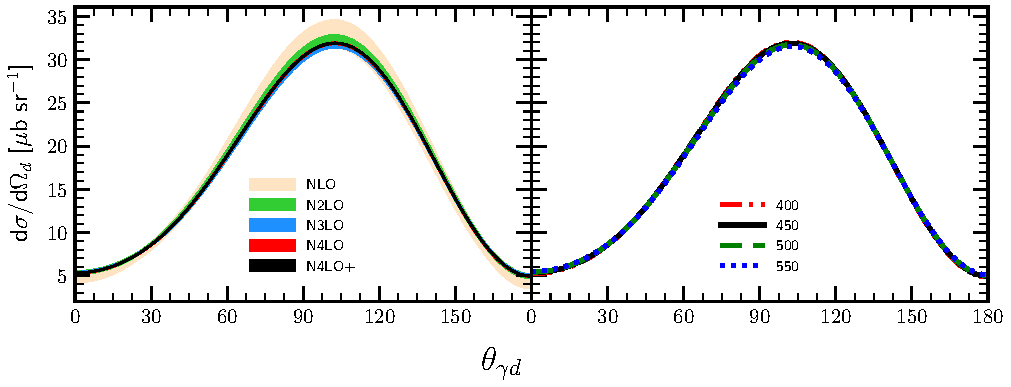
\includegraphics[width=0.9\textwidth]{Figures_HE/CROSS_nd_trunc_30mev.pdf}
        \end{center}
        \caption{Differential cross section for the
        two-body photodisintegration of $^3$He as a function of the $d-\gamma$ angle in c.m..
        The initial photon energy $\text{E}_\gamma=\SI{30}{\mev}$ and NN with 2NF was used.}
        \label{CROSS_nd_30}
    \end{figure}


    \begin{figure}[h]
        \begin{center}
        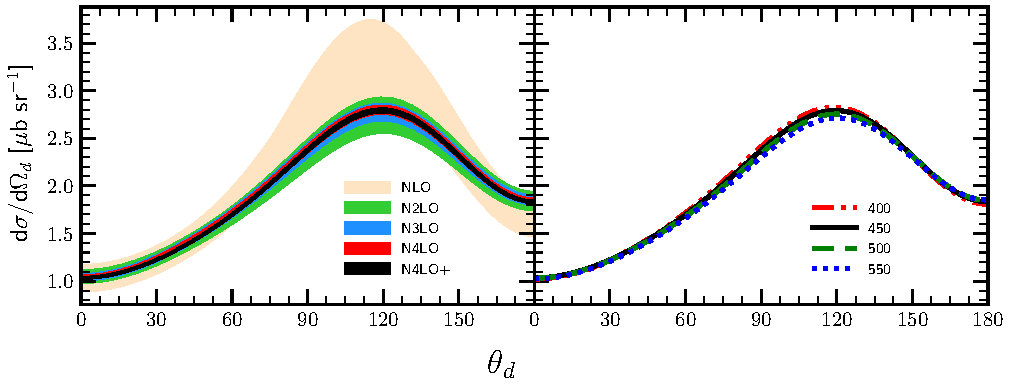
\includegraphics[width=0.9\textwidth]{Figures_HE/CROSS_nd_trunc_100mev.pdf}
        \end{center}
        \caption{The same as in the \fig{CROSS_nd_30} but 
        for the photon energy E$_\gamma=\SI{100}{\mev}$}
        \label{CROSS_nd_100}
    \end{figure}

    \clearpage
\section{Triton photodisintegration}
    \label{sec:triton_results}
    
    
    In this section, I will discuss results for $^3\text{H} \rightarrow n + n + p$ process in the case when two neutrons are detected 
    and similarly to the previous chapter, I present the convergence of predictions 
    and their cut-off dependence. 

    In the \fig{CROSS_Triton_EXCL_30_15_0_15_180} I present a differential cross section 
    $\frac{d^5\sigma}{d\Omega_1d\Omega_2dS}$ as a function of the S arc length.
    The photon energy is  E$_\gamma=\SI{30}{\mev}$ and the kinematic configuration
    $\theta_1 = \ang{15}$, $\phi_1 = \ang{0}$,
    $\theta_2 = \ang{15}$, $\phi_2 = \ang{180}$; predictions have been obtained without 3NF.
    We see that only \gls{nlo} and \gls{n2lo} introduce relatively large truncation errors.
    The maximal width of a band for NLO is \SI{30.95}{\percent} at $S=\SI{10}{\mev}$,
    for \gls{n2lo} it is \SI{6.79}{\percent} at the same point and it is gradually decreasing
    coming to \SI{0.10}{\percent} at \gls{n4lo+}.
    The cut-off spread around maxima values is \SI{6.25}{\percent} (at $S=\SI{4}{\mev}$) and it is
    \SI{1.81}{\percent} at $S=\SI{10}{\mev}$.

    \begin{figure}[h]
        \begin{center}
            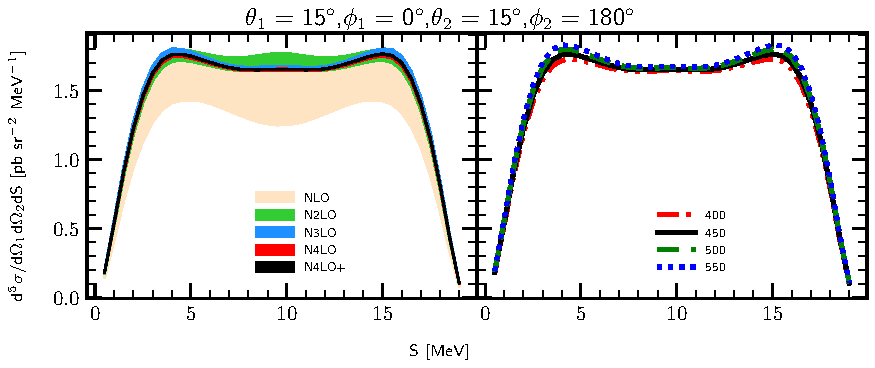
\includegraphics[width=0.9\textwidth]{Figures_Triton/CROSS_excl_trunc_30mev_15_0_15_180_2NF.pdf}
            \end{center}
            \caption{The five-fold differential cross section for the photon 
            energy E$_\gamma=\SI{30}{\mev}$ for the kinematic configuration
            $\theta_1 = \ang{15}$, $\phi_1 = \ang{0}$,
            $\theta_2 = \ang{15}$, $\phi_2 = \ang{180}$ with detected particles proton (number 1) and neuteron (number 2).
            The left figure presents truncation error bands obtained using potential
            with chiral orders from \gls{nlo} to \gls{n4lo+}, and with
            cut-off parameter $\Lambda=\SI{450}{\mev}$.
            The right figure presents a cut-off dependence at \gls{n4lo+}.
            Results are obtained with two-nucleon force only and \gls{snc} current plus Siegert.}
            \label{CROSS_Triton_EXCL_30_15_0_15_180}
    \end{figure}

    At bigger energy E$_\gamma=\SI{100}{\mev}$ demonstrated in the \fig{CROSS_Triton_EXCL_100mev_15_0_15_180},
    the truncation band at the maximum point $S=\SI{10}{\mev}$ for NLO is \SI{50.26}{\percent}
    decreases to \SI{2.00}{\percent} at \gls{n4lo+}.
    The cut-off spread also becomes larger with increasing energy value: \SI{9.52}{\percent}
    at the same maximum.

    The truncation error bands and cut-off dependence are very similar to what was found for
    the three-body Helium-3 photodisintegration and the relative errors 
    have similar magnitudes.

    \begin{figure}[h]
        \begin{center}
            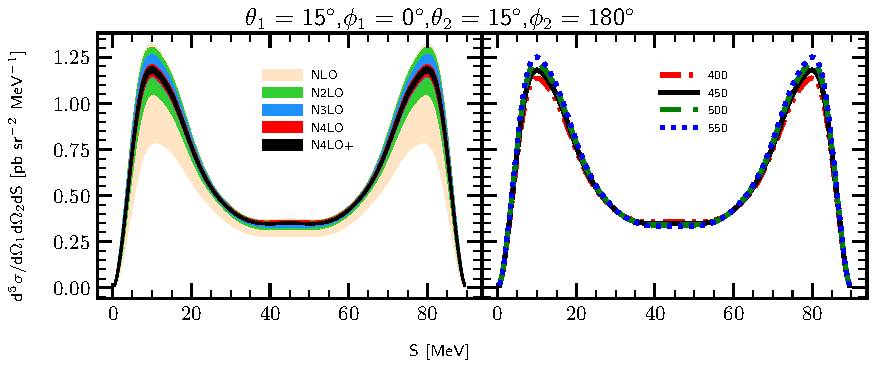
\includegraphics[width=0.9\textwidth]{Figures_Triton/CROSS_excl_trunc_100mev_15_0_15_180_2NF.pdf}
            \end{center}
            \caption{The same as in the \fig{CROSS_Triton_EXCL_30_15_0_15_180} but for the photon energy
            E$_\gamma = \SI{100}{\mev}$.}
            \label{CROSS_Triton_EXCL_100mev_15_0_15_180}
    \end{figure}



    Results for other angular configurations with E$_\gamma=\SI{30}{\mev}$ and at 
    $\theta_1 = \ang{75}$, $\phi_1 = \ang{75}$,
    $\theta_2 = \ang{75}$, $\phi_2 = \ang{105}$ are
    demonstrated in \fig{CROSS_Triton_EXCL_75_75_75_105}.
    Both truncation errors and cut-off dependence are smaller with such configuration:
    the relative  width of the truncation band at \gls{nlo} is \SI{9.39}{\percent}
    (at the maximum point $S=\SI{8}{\mev}$) and drops to only \SI{0.1}{\percent}
    at \gls{n4lo+}. The relative cut-off spread is \SI{0.93}{\percent} at the same point.

    At the bigger energy E$_\gamma=\SI{100}{\mev}$ demonstrated in \fig{CROSS_Triton_EXCL_100mev_75_75_75_105}
    uncertainties grow. The truncation bands are \SI{44.42}{\percent} and 
    \SI{2.09}{\percent} (at \gls{nlo} and \gls{n4lo+} respectively) and
    the cut-off spread is \SI{13.04}{\percent} (all at $S=\SI{35}{\mev}$ in maximum).


    \begin{figure}[h]
        \begin{center}
            \includegraphics[width=0.9\textwidth]{Figures_Triton/CROSS_excl_trunc_30mev_75_75_75_105_2NF.pdf}
            \end{center}
            \caption{The same as in the \fig{CROSS_Triton_EXCL_30_15_0_15_180} but for the kinematic
            configuration with
            $\theta_1 = \ang{75}$, $\phi_1 = \ang{75}$,
            $\theta_2 = \ang{75}$, $\phi_2 = \ang{105}$.}
            \label{CROSS_Triton_EXCL_75_75_75_105}
    \end{figure}


    \begin{figure}[h]
        \begin{center}
            \includegraphics[width=0.9\textwidth]{Figures_Triton/CROSS_excl_trunc_100mev_75_75_75_105_2NF.pdf}
            \end{center}
            \caption{The same as in the \fig{CROSS_Triton_EXCL_75_75_75_105} but for the photon energy
            E$_\gamma = \SI{100}{\mev}$.}
            \label{CROSS_Triton_EXCL_100mev_75_75_75_105}
    \end{figure}

    Similar trends are present also in other examples, demonstrated for the comparison in
    Figs.~\ref{CROSS_Triton_EXCL_15_105_15_75}-\ref{CROSS_Triton_EXCL_100mev_165_15_15_165}.

    \begin{figure}[h]
        \begin{center}
            \includegraphics[width=0.9\textwidth]{Figures_Triton/CROSS_excl_trunc_30mev_15_105_15_75_2NF.pdf}
            \end{center}
            \caption{The same as in the \fig{CROSS_Triton_EXCL_75_75_75_105} but for the kinematic
            configuration with
            $\theta_1 = \ang{15}$, $\phi_1 = \ang{105}$,
            $\theta_2 = \ang{15}$, $\phi_2 = \ang{75}$.}
            \label{CROSS_Triton_EXCL_15_105_15_75}
    \end{figure}


    \begin{figure}[h]
        \begin{center}
            \includegraphics[width=0.9\textwidth]{Figures_Triton/CROSS_excl_trunc_100mev_15_105_15_75_2NF.pdf}
            \end{center}
            \caption{The same as in the \fig{CROSS_Triton_EXCL_15_105_15_75} but for the photon energy
            E$_\gamma = \SI{100}{\mev}$.}
            \label{CROSS_Triton_EXCL_100mev_15_105_15_75}
    \end{figure}

    \begin{figure}[h]
        \begin{center}
            \includegraphics[width=0.9\textwidth]{Figures_Triton/CROSS_excl_trunc_30mev_45_75_45_105_2NF.pdf}
            \end{center}
            \caption{The same as in the \fig{CROSS_Triton_EXCL_15_105_15_75} but for the kinematic
            configuration with
            $\theta_1 = \ang{45}$, $\phi_1 = \ang{75}$,
            $\theta_2 = \ang{45}$, $\phi_2 = \ang{105}$.}
            \label{CROSS_Triton_EXCL_45_75_45_105}
    \end{figure}


    \begin{figure}[h]
        \begin{center}
            \includegraphics[width=0.9\textwidth]{Figures_Triton/CROSS_excl_trunc_100mev_45_75_45_105_2NF.pdf}
            \end{center}
            \caption{The same as in the \fig{CROSS_Triton_EXCL_45_75_45_105} but for the photon energy
            E$_\gamma = \SI{100}{\mev}$.}
            \label{CROSS_Triton_EXCL_100mev_45_75_45_105}
    \end{figure}

    \begin{figure}[h]
        \begin{center}
            \includegraphics[width=0.9\textwidth]{Figures_Triton/CROSS_excl_trunc_30mev_165_15_15_165_2NF.pdf}
            \end{center}
            \caption{The same as in the \fig{CROSS_Triton_EXCL_45_75_45_105} but for the kinematic
            configuration with
            $\theta_1 = \ang{165}$, $\phi_1 = \ang{15}$,
            $\theta_2 = \ang{15}$, $\phi_2 = \ang{165}$.}
            \label{CROSS_Triton_EXCL_165_15_15_165}
    \end{figure}


    \begin{figure}[h]
        \begin{center}
            \includegraphics[width=0.9\textwidth]{Figures_Triton/CROSS_excl_trunc_100mev_165_15_15_165_2NF.pdf}
            \end{center}
            \caption{The same as in the \fig{CROSS_Triton_EXCL_165_15_15_165} but for the photon energy
            E$_\gamma = \SI{100}{\mev}$.}
            \label{CROSS_Triton_EXCL_100mev_165_15_15_165}
    \end{figure}
        
        
    \clearpage
\section{Pion absorption from the lowest atomic orbital}
\label{sec:pion_results}

\subsection{Pion absorption in $^2$H}


\begin{figure}[h]
        \begin{center}
        \includegraphics[width=0.6\textwidth]{PlotData/PION/Dalitz_maps/figures/Gamma_nn.pdf}
        \end{center}
        \caption{
            Absorption rate for the $\pi^- + {^2{\rm H}} \rightarrow n + n$ reaction.
            The rates were calculated using the \gls{sms} force with different chiral orders and cut-off values.
            The results were obtained using the single-nucleon transition operator and 
            supplemented by two-nucleon contributions at the leading order.
            The figure shows the results obtained using the plane wave (PW) plus
            two-neutron rescattering (Full) parts.
            The experimental value is extracted from the hadronic
            ground-state broadening in pionic deuterium and is taken from Refs.~\cite{Strauch2010,Strauch2011}.}
        \label{Gamma_nn}
    \end{figure}

    In \fig{Gamma_nn} the absorption rate $\Gamma_{nn}$ is shown for the process $\pi^- + {^2{\rm H}} \rightarrow n + n$
    as a function of the chiral order (horizontal axis) and the cutoff parameter (different lines) 
    together with experimental data extracted from \cite{Strauch2010,Strauch2011}.
    We see a significant difference between
    predictions obtained using different $\Lambda$. The impact of chiral orders is large at \gls{lo}
    and \gls{nlo} (each subsequent order differs from the previous 
    by $\sim\SI{40}{\percent}$ and $\sim\SI{30}{\percent}$, respectively) 
    and is gradually decreasing, and \gls{n3lo}-\gls{n4lo}-\gls{n4lo+} steps are almost invisible
    (the relative difference between subsequent orders is $\sim\SI{5}{\percent}$).
    The comparison with experimental data shows that our predictions converge to a correct value coming 
    closely to it all large chiral orders and $\Lambda$s except $\Lambda = \SI{450}{\mev}$ 
    which is clearly separated from other predictions. The bias $\Gamma^{550}_{nn} - \Gamma^{exp}_{nn}$
    is still \SI{0.178e15}{s^{-1}} which is \SI{12.7}{\percent}.
    Such a result reveals that NN interaction with $\Lambda = \SI{450}{\mev}$  is inadequate in data description. 
    However, using it gives an additional measure of uncertainty related to the cut-off parameter value.


    \subsection{Pion absorption in $^3$He}
    
    In \fig{Gamma_pnn} and \ref{Gamma_nd} the total pion absorption rates are presented as a function
    of the chiral order and for different values of the cut-off parameter
    for $\pi^- + ^3\text{He} \rightarrow p + n + n$ 
    and $\pi^- + ^3\text{He} \rightarrow n + d$ reactions, respectively.
    Both figures show that with fixed chiral order the arrangement 
    of absorption rates obtained with various values of the cut-off parameter
    remains the same, namely with increasing $\Lambda$, the absorption rate decreases. The only exception in both cases 
    appears at \gls{n3lo} where prediction with $\Lambda = \SI{550}{\mev}$ goes above other predictions.
    At the next order, \gls{n4lo}, it comes back to the usual arrangement.
    This behavior may be connected to the $^3$He wave function resulting from the
    3NF used for the calculation.
    In order to prove that, I show in \fig{proton_rad}
    a corresponding figure for a $^3$He proton radius $r_p$ calculated with 
    and without 3NF (left and right panels, respectively). Results obtained with the 3NF show
    also a deviation at \gls{n3lo} where $\Lambda=\SI{550}{\mev}$ and $\Lambda=\SI{500}{\mev}$ are 
    very close to each other while for the radius computed without the 3NF a clear separation is present.
    Nevertheless, the spread of predictions concerning
    the cut-off values seen in \fig{proton_rad} is much smaller
    with the 3NF and deviation seems to be not crucial as the total difference
    between predictions in this case is very small.

    There are also experimental data for the $\Gamma_{pnn}$ and $\Gamma_{nd}$ available on the market.
    As it was discussed in \cite{golak_pion}, experimental data for the $\Gamma_{pnn}$ and $\Gamma_{nd}$ 
    can be extracted from \cite{SCHWANNER1984,McCarthy1975,truol1974} and it is

    \begin{eqnarray}\label{Gam_He_exp}
        \Gamma_{pnn} ^{\rm exp.} & =& (2.47\pm 0.65)\times 10^{16} \, {\rm s^{-1}}\\
        \Gamma_{nd}^{\rm exp.} & =  & (6.8\pm 1.9)\times 10^{15} \, {\rm s^{-1}}.
    \end{eqnarray}

    My predictions can be summarized as follows:

    \begin{eqnarray}\label{Gam_nd_our}
        \Gamma_{pnn}  & =& (1.28^{+ 0.29}_{-0.14} \pm 1.02)\times 10^{16} \, {\rm s^{-1}}\\ \label{Gam_nd_pnn_our}
        \Gamma_{nd} & =  & (2.0^{+1.0}_{-0.6}\pm 1.6)\times 10^{15} \, {\rm s^{-1}}\\ \label{Gam_pnn_our}
    \end{eqnarray}
    where the first error is related to the cut-off parameter and the second one to the chiral order (truncation error).

    We see that our predictions, presented in Figs.~\ref{Gamma_pnn} and \ref{Gamma_nd}, are 
    smaller than experimental values, but they overlap each other within the uncertainty range, giving large experimental errors as well as theoretical ones.



    \begin{figure}[h]
        \begin{center}
        \includegraphics[width=0.6\textwidth]{PlotData/PION/Dalitz_maps/figures/Gamma_pnn.pdf}
        \end{center}
        \caption{Absorption rate for $\pi^- + ^3\text{He} \rightarrow p + n + n$ reaction as a function
        of the chiral order and with different values of the cut-off parameter $\Lambda$.
        Predictions were obtained with the \gls{sms} NN interaction at a given order combined
        with \gls{n2lo} 3NF.}
        \label{Gamma_pnn}
    \end{figure}

    \begin{figure}[h]
        \begin{center}
        \includegraphics[width=0.6\textwidth]{PlotData/PION/Dalitz_maps/figures/Gamma_nd.pdf}
        \end{center}
        \caption{The same as in \fig{Gamma_pnn}, but for $\pi^- + ^3\text{He} \rightarrow n + d$ reaction.}
        \label{Gamma_nd}
    \end{figure}

    \begin{figure}[h]
        \begin{center}
        \includegraphics[width=0.99\textwidth]{PlotData/PION/Dalitz_maps/figures/proton_radius_mt31_3NF.pdf}
        \end{center}
        \caption{ Proton radius $r_p$ for $^3$He nuclei as a function of the chiral order calculated with
        different values of the cut-off parameter $\Lambda$. The radius was calculated with 2NF and 3NF (left panel)
        or with 2NF only (right panel).}
        \label{proton_rad}
    \end{figure}


    By its nature, the total absorption rates cannot deliver details
    on the distribution of contributions arising from various dynamical ingredients
    to the absorption process in the phase space. Thus in the following, I show 
    various intensity plots revealing phase-space regions of special interest.

    Let me remind that in the case of absorption rates, only two kinetical variables are
    necessary to define the exclusive kinematical configuration. That is, because for that
    process there is full rotational symmetry, as none of the vectors define the $\hat(z)$-axis.


    In Figs.~\ref{pion_map_E1E2_cutoff} and \ref{pion_map_xy_cutoff} I show such
    intensity plots for the double differential absorption rates
    $d^2 \Gamma_{pnn}/dE_1dE_2$ for the $\pi^- + ^3\text{He} \rightarrow p + n + n$
    process as functions of the nucleons energies (assuming nucleon number 1 to be a proton) and 
    of the Dalitz coordinates ($x$ and $y$), respectively.

    The coordinates $x$ and $y$ are defined as:

    \begin{align}
        x &= 3 (E_1 + 2E_2 - E)/E, \nonumber\\
        y &= (3E_1 - E)/E,
        \label{dalitz_xy}
    \end{align}
    where $E$ is a total kinetic 3N energy. 
    These coordinates are restricted to the region where $r^2 \equiv x^2 + y^2 \leq 1$.

    Each of the two figures consists of four panels representing predictions obtained with different 
    values of the cut-off parameter $\Lambda$. The difference between predictions which can be immediately
    noticed with the naked eye is that the area of the central region (corresponding to the smallest rates)
    becomes larger with increasing $\Lambda$. It coheres to what we saw in \fig{Gamma_pnn}
    where the total absorption rate was inversely correlated with the cut-off parameter. The dominant contribution
    comes from the region with the lowest proton energy values of $E_1 \rightarrow 0$ where both neutron energies 
    have similar large values.
    This is a situation of quasi-free scattering(QFS) - when a proton is a spectator and both neutrons share equally all energy. 

    Another region with a high absorption rate is the neutron-neutron final state interaction configuration (FSI(nn)).
    It is located at high $E_1$ values when a proton gets two-thirds part of the total energy while neutrons both get
    one-sixth of it.
    It means that proton's kinetic energy is four times larger than neutron's.
    % (what is visible in the figure). 
    In \fig{pion_map_E1E2_cutoff} we see this region at the very right region (with $E_1 \rightarrow 85$)
    with rapid growth of the absorption rate and it is observed at every value of the cut-off parameter. The very same region 
    is presented in  \fig{pion_map_xy_cutoff} at $y \rightarrow 1$.

    In \cite{golak_pion} we have shown the comparison of our predictions with one more experimental data,
    from \cite{Gotta1995}. In that paper, the authors consider four specific regions ($I_i$ for $i=1,2,3,4$) and give experimental results
    for each of them separately. The renormalization procedure was applied to our predictions in order to compare results with experimental data. Following \cite{Gotta1995}, we divide the predictions for each particular region ($\Gamma_i$) by the total value $\sum_{i=1}^{4}\Gamma_i$. Results are presented in the Table \ref{tableregions_norm}.

    \begin{table}%[H] add [H] placement to break table across pages
        \centering
        \caption{Absorption rates in the four regions 
        of the phase space $I_i$ defined in 
            Ref.~\cite{Gotta1995} 
        for the $\pi^- + {^3{\rm He}} \rightarrow p + n + n $ reaction
        calculated with 
        the chiral \gls{sms} NN potential supplemented by 3NF at \gls{n2lo}
        with different values of the cutoff parameter $\Lambda$.}
        \begin{tabular}{|c|c|c|c|c|}
            \hline\hline
                & \multicolumn{4}{c|}{Normalized absorption rates $\Gamma_{i}$} \\ 
                                \cline{2-5}
            \hline
                $\Lambda$ (MeV)                             &      $I_1$ &      $I_2$ &      $I_3$ &      $I_4$ \\ 
            \hline
            %
            400   &  \;\;0.804\;\; &\;\; 0.152\;\;  &\;\;\ 0.029\;\;  & \;\;0.016\;\; \\
            450   &  0.797  & 0.152  & 0.032  & 0.019 \\
            500   &  0.792  & 0.152  & 0.035  & 0.021 \\
            550   &  0.793  & 0.151  & 0.036  & 0.020  \\
            %
            \hline\hline
            Gotta \textit{et al.} \cite{Gotta1995} &    0.844& 0.099& 0.033& 0.023 \\
            \hline\hline
        \end{tabular}
        \label{tableregions_norm}
    \end{table}

    We see that our predictions are very close to experimental results and retrieve the same pattern of the absorption rate distribution over the regarded regions.
        
    
    
        \begin{figure}[h]
            \begin{center}
            \includegraphics[width=0.7\textwidth]{PlotData/PION/Dalitz_maps/figures/Dalitz_map_pnn_E1E2_cutofs.pdf}
            \end{center}
            \caption{Intensity plots for the double differential absorption rates
            $d^2 \Gamma_{pnn}/dE_1dE_2$ for the $\pi^- + ^3\text{He} \rightarrow p + n + n$ process, obtained using the SMS NN potential
            with all contributions possible: plane wave + rescattering, 1NC + 2N, 2NF+3NF.
            Each panel presents predictions obtained with different values of the cut-off parameter $\Lambda$:
            from $\Lambda=\SI{400}{\mev}$ (upper left) to $\Lambda=\SI{550}{\mev}$ (lower right). Nucleon 1 is a proton.}
            \label{pion_map_E1E2_cutoff}
        \end{figure}

    \begin{figure}[h]
        \begin{center}
        \includegraphics[width=0.7\textwidth]{PlotData/PION/Dalitz_maps/figures/Dalitz_map_pnn_xy_cutofs.pdf}
        \end{center}
        \caption{The same as in \fig{pion_map_E1E2_cutoff} but for the double differential absorption rates
        $d^2 \Gamma_{pnn}/dxdy$.}
        \label{pion_map_xy_cutoff}
    \end{figure}

    Next in Figs.~\ref{pion_map_E1E2_cutoff_PW} and \ref{pion_map_xy_cutoff_PW} 
    I show similar intensity plots for the predictions obtained with plane wave component only (without rescattering part).
    They reveal that
    the difference of predictions obtained without rescattering part with ones including it
    (Figs.~\ref{pion_map_E1E2_cutoff} and \ref{pion_map_xy_cutoff}) is very large. 
    Predicted values are a few times larger and the distribution of dominant areas is completely different.
    The FSI(nn) region is not presented here
    in the sense that there is no peak concerning other regions.
    That is natural, as the FSI(nn) peak arises from strong interaction in the final state,
    which by definition is not in the plane wave approximation.
    On the contrary, the QFS region is presented.
    Results of Figs.~\ref{pion_map_E1E2_cutoff_PW} and \ref{pion_map_xy_cutoff_PW}
    tell us that one has to take into account the rescattering part in order to obtain
    realistic predictions for that process.  

    \begin{figure}[h]
        \begin{center}
        \includegraphics[width=0.7\textwidth]{PlotData/PION/Dalitz_maps/figures/Dalitz_map_pnn_E1E2_cutofs_PWIAS.pdf}
        \end{center}
        \caption{Intensity plots for the double differential absorption rates
        $d^2 \Gamma_{pnn}/dE_1dE_2$ for the $\pi^- + ^3\text{He} \rightarrow p + n + n$
        process obtained using the SMS NN potential at \gls{n4lo+} supplemented by \gls{n2lo} 3NF
        with plane wave part only (without rescattering).
        All other contributions are the same as in \fig{pion_map_E1E2_cutoff}: 1NC + 2N and 2NF+3NF.
        Each panel presents predictions obtained with different values of the cut-off parameter $\Lambda$:
        from $\Lambda=\SI{400}{\mev}$ (upper left) to $\Lambda=\SI{550}{\mev}$ (lower right). Nucleon 1 is a proton.}
        \label{pion_map_E1E2_cutoff_PW}
    \end{figure}

    \begin{figure}[h]
        \begin{center}
        \includegraphics[width=0.7\textwidth]{PlotData/PION/Dalitz_maps/figures/Dalitz_map_pnn_xy_cutofs_PWIAS.pdf}
        \end{center}
        \caption{The same as in \fig{pion_map_E1E2_cutoff_PW} but for the double differential absorption rates
        $d^2 \Gamma_{pnn}/dxdy$.}
        \label{pion_map_xy_cutoff_PW}
    \end{figure}

    Results have been obtained with plane wave plus rescattering parts but with the single nucleon current only
    are presented in Figs.~\ref{pion_map_E1E2_cutoff_1NC} and \ref{pion_map_xy_cutoff_1NC}.
    As previously, each panel in the figures presents predictions obtained with different values of the cut-off parameter $\Lambda$.
    In contrast to the combinations shown above, the change in the cut-off value has a larger impact here:
    we observe that there is a different pattern in each panel. It does not change dramatically, but 
    two peaks inside the figure become more or less clear. On the other hand, the distribution of 
    the absorption rate is very different from the one, obtained with a more complete components setup 
    (Figs.~\ref{pion_map_E1E2_cutoff} and \ref{pion_map_xy_cutoff}).


    \begin{figure}[h]
        \begin{center}
        \includegraphics[width=0.7\textwidth]{PlotData/PION/Dalitz_maps/figures/Dalitz_map_pnn_E1E2_cutofs_1NC.pdf}
        \end{center}
        \caption{Intensity plots for the double differential absorption rates
        $d^2 \Gamma_{pnn}/dE_1dE_2$ for the $\pi^- + ^3\text{He} \rightarrow p + n + n$
        process obtained using the SMS NN potential at \gls{n4lo+} supplemented by \gls{n2lo} 3NF
        with \gls{snc} only (without 2N) currents.
        All other contributions are the same as in \fig{pion_map_E1E2_cutoff}: PWIAS+RESC and 2NF+3NF.
        Each panel presents predictions obtained with different values of the cut-off parameter $\Lambda$:
        from $\Lambda = \SI{400}{\mev}$ (upper left) to $\Lambda = \SI{550}{\mev}$ (lower right). Nucleon 1 is a proton.}
        \label{pion_map_E1E2_cutoff_1NC}
    \end{figure}

    \begin{figure}[h]
        \begin{center}
        \includegraphics[width=0.7\textwidth]{PlotData/PION/Dalitz_maps/figures/Dalitz_map_pnn_xy_cutofs_1NC.pdf}
        \end{center}
        \caption{The same as in \fig{pion_map_E1E2_cutoff_1NC} but for the double differential absorption rates
        $d^2 \Gamma_{pnn}/dxdy$.}
        \label{pion_map_xy_cutoff_1NC}
    \end{figure}

    Figs.~\ref{pion_map_E1E2_order} and \ref{pion_map_xy_order} show prediction obtained using similar
    dynamical components
    as in Figs.~\ref{pion_map_E1E2_cutoff} and \ref{pion_map_xy_cutoff}, but each panel includes
    predictions obtained with different chiral orders of the \gls{sms} potential.
    We see that predictions are not sensitive to the chiral order and even \gls{n2lo} predictions
    are pretty much similar to ones obtained with the most advanced \gls{n4lo} potential.
     
    
    \begin{figure}[h]
        \begin{center}
            \includegraphics[width=0.7\textwidth]{PlotData/PION/Dalitz_maps/figures/Dalitz_map_pnn_E1E2_orders.pdf}
        \end{center}
        \caption{Intensity plots for the double differential absorption rates
        $d^2 \Gamma_{pnn}/dE_1dE_2$ for the $\pi^- + ^3\text{He} \rightarrow p + n + n$
        process obtained using the SMS potential at \gls{n4lo+}
        with all contributions possible: plane wave + rescattering, 1NC + 2N, 2NF+3NF.
        Each panel presents predictions obtained with different chiral orders of the \gls{sms} NN potential:
        from \gls{n2lo} (upper left) to \gls{n4lo+} (lower right) and with $\Lambda = \SI{450}{\mev}$.
        Nucleon 1 is a proton. 3NF was taken ar \gls{n2lo} in each case.}
        \label{pion_map_E1E2_order}
    \end{figure}

    \begin{figure}[h]
        \begin{center}
        \includegraphics[width=0.7\textwidth]{PlotData/PION/Dalitz_maps/figures/Dalitz_map_pnn_xy_orders.pdf}
        \end{center}
        \caption{The same as in \fig{pion_map_E1E2_order} but for the double differential absorption rates
        $d^2 \Gamma_{pnn}/dxdy$.}
        \label{pion_map_xy_order}
    \end{figure}

    
    Presented above intensity plots correspond to exclusive processes with two particles detected.
    Now we would like to test if the same behavior of the capture rate is observed for
    the semi-inclusive observables.
    Thus following figures demonstrate the same phenomena but from a different point of view.
    Namely in \fig{pion_GdEp} I show differential absorption rate $d\Gamma_{pnn} /d\text{E}_p$
    that is the same as in e.g. \fig{pion_map_E1E2_order}, but integrated over E$_n$.
    All the results are obtained with the most advanced setup (plane wave + rescattering, 1NC + 2N, 2NF+3NF).
    The left panel consists of the results with $\Lambda=\SI{450}{\mev}$ and each curve corresponds 
    to a particular chiral order. An interesting region here is a maximum
    of $d\Gamma_{pnn} /d\text{E}_p$  which corresponds
    to the bottom part of the circles from \fig{pion_map_E1E2_order}. At the point of maximum
    \gls{n2lo} prediction distinguishes from other results as its point of maximum is noticeably higher.
    At $\text{E}_p = \SI{0.92}{\mev}$ (maximum point) the value of \gls{n2lo} is
    \num{1.37} times larger than one from \gls{n4lo+} (\SI{3.44e+17}{fm.\s^{-1}}
    vs \SI{2.52e+17}{fm.\s^{-1}}) - the relative difference is \SI{31.1}{\percent}.
    At the same time, the relative difference between all the predictions except for \gls{n2lo}
    is \SI{8.3}{\percent}.

    The right panel of the \fig{pion_GdEp} shows a cut-off dependence of the predictions obtained
    with the \gls{sms} NN chiral potential at \gls{n4lo+} supplemented by \gls{n2lo} 3NF.
    In this case, the maximum point is interesting as well.
    We see that predictions with $\Lambda=\SI{500}{\mev}$ and $\SI{550}{\mev}$ are quite close to each other:
    the relative difference between them at $\text{E}_p = \SI{0.92}{\mev}$ is only \SI{1.5}{\percent}.
    In turn the spread between $\Lambda=\SIlist{400;450;500}{\mev}$ is \SI{40}{\percent} (at the same $E_p$).
    This cut-off dependence is hidden when looking at the colormaps 
    \fig{pion_map_E1E2_cutoff}, but from this perspective it is clearly presented.
    Anyway, the highest $\Lambda$, the biggest $d\Gamma_{pnn} /d\text{E}_p$ is seen.
    That observable could be an intensity test for the cut-off value, however, it requires measurement
    at low proton energy ($\sim$\SIrange{0.8}{1.0}{MeV}) which is an experimental challenge.

    \begin{figure}[h]
        \begin{center}
        \includegraphics[width=0.9\textwidth]{PlotData/PION/Dalitz_maps/figures/3HE_dGdEp.pdf}
        \end{center}
        \caption{Differential absorption rate $d\Gamma_{pnn} /d\text{E}_p$ 
        as a function of the proton energy E$_p$ for the 
        $\pi^- + ^3\text{He} \rightarrow p + n + n$ process.
        Left panel shows results obtained with the NN \gls{n2lo} (green dashed line),
        \gls{n3lo} (blue dotted line), \gls{n4lo} (red dashed-double-dotted line)
        and \gls{n4lo+} (black solid line) chiral orders plus \gls{n2lo} 3NF, and with $\Lambda = \SI{450}{\mev}$.
        The right panel includes results obtained with the \gls{n4lo+} \gls{sms} NN potential plus \gls{n2lo} 3NF
        with different values of the $\Lambda$: \SI{400}{\mev} (red dashed-double-dotted line),
        $\Lambda$: \SI{450}{\mev} (black solid line),
        $\Lambda$: \SI{500}{\mev} (green dashed line line) and
        $\Lambda$: \SI{550}{\mev} (blue dotted line).
        All predictions were obtained with "FULL-(1NC+2N)-(2NF+3NF)" setup.}
        \label{pion_GdEp}
    \end{figure}

    Similarly in \fig{pion_dGdEn} $d\Gamma_{pnn} /d\text{E}_n$ is presented. We observe similar trends as above
    (they are also shown up at the maximum point, which is around E$_n = \SI{66.9}{\mev}$ now):
    the difference between \gls{n2lo} and \gls{n4lo+} predictions at this point is \SI{29.0}{\percent};
    the relative difference between all the predictions except for \gls{n2lo}
    is much smaller, but still is approx. \SI{7.5}{\percent};
    the \gls{n4lo+} predictions are also very similar for $\Lambda=\SIlist{500;550}{\mev}$ (the spread is \SI{1.6}{\percent})
    while all remaining predictions are quite distinguished - the spread is \SI{39.1}{\percent}.
    I find that observable very interesting in the context of experimental studies as a measurement of neutron at
    $E\eqsim\SI{70}{\mev}$ is nowadays within our reach. 


    \begin{figure}[h]
        \begin{center}
        \includegraphics[width=0.9\textwidth]{PlotData/PION/Dalitz_maps/figures/3HE_dGdEn.pdf}
        \end{center}
        \caption{The same as in \fig{pion_GdEp} but for the differential absorption rate $d\Gamma_{pnn} /d\text{E}_n$
        as a function of the neutron energy E$_n$.}
        \label{pion_dGdEn}
    \end{figure}

    Moving to the next figures, \fig{pion_dGdEr} and \fig{pion_dGdphi}, I show 1-dim dependence of the
    absorption rate on the Dalitz coordinates $r = \sqrt{x^2 + y^2}$  and $\phi = \arctan \frac{y}{x}$, respectively.
    A similar trend is preserved, namely chiral order figures show that \gls{n2lo} predictions
    outstand from all other predictions, and noticeable cut-off dependence is observed.

    In general, we can conclude that predictions are converged starting from the \gls{n3lo} chiral order (for NN force) as
    most of the demonstrated results show that the difference between \gls{n3lo}, \gls{n4lo} and 
    \gls{n4lo+} is negligible. At the same time, we observe a strong cut-off dependence with
    predictions obtained with $\Lambda=\SIlist{500;550}{\mev}$ being very similar,
    but with a large spread of all the rest results.
    This nature of the cut-off dependence is also reflected in the total absorption 
    rate, presented in \fig{Gamma_pnn}. 

    \begin{figure}[h]
        \begin{center}
        \includegraphics[width=0.9\textwidth]{PlotData/PION/Dalitz_maps/figures/3HE_dGdr.pdf}
        \end{center}
        \caption{The same as in \fig{pion_GdEp} but for the differential absorption rate $d\Gamma_{pnn} /dr$
        as a function of the parameter $r$ of the Dalitz coordinates: $r = \sqrt{x^2 + y^2}$.}
        \label{pion_dGdEr}
    \end{figure}

    \begin{figure}[h]
        \begin{center}
        \includegraphics[width=0.9\textwidth]{PlotData/PION/Dalitz_maps/figures/3HE_dGdphi.pdf}
        \end{center}
        \caption{The same as in \fig{pion_dGdEr} but for the differential absorption rate $d\Gamma_{pnn} /d\phi$
        as a function of the azimuthal angle $\phi$ of the Dalitz coordinates: $\phi = \arctan \frac{y}{x}$.}
        \label{pion_dGdphi}
    \end{figure}


    \clearpage
    \subsection{Pion absorption in $^3$H}

    In this subsection, I will show the results of calculations for
    the $\pi^- + ^3\text{H} \rightarrow n + n + n$ process.
    In this case, only a three-body breakup is allowed as 
    no two-body configuration can be composed out of three neutrons.
    
    The total absorption rate $\Gamma_{nnn}$ for that process is shown in \fig{Gamma_nnn}
    as a function of the chiral order of the \gls{sms} NN potential while each curve represents
    different cut-off values used to obtain the prediction. 
    The most advanced dynamical model was used in this case, namely Plane wave plus rescattering part,
    both single- and two-nucleon currents and two-nucleon plus three-nucleon interaction.

    Similarly to the three-body break-up of $^3$He, we see that with each subsequent chiral order
    predictions become closer to each other, so the cut-off dependence gets weaker.
    Also, the prediction with $\Lambda=\SI{550}{\mev}$ at \gls{n3lo} is
    strangely above the prediction with $\Lambda=\SI{500}{\mev}$.
    We can also notice, that at \gls{n4lo}
    predictions with cut-off values \SI{500}{\mev} and \SI{550}{\mev}
    are much closer to each other than to results obtained with other $\Lambda$s.

    \begin{figure}[h]
        \begin{center}
        \includegraphics[width=0.6\textwidth]{PlotData/PION/Dalitz_maps/figures/Gamma_nnn.pdf}
        \end{center}
        \caption{Absorption rate for $\pi^- + ^3\text{H} \rightarrow n + n + n$ reaction as a function
        of the chiral order with different values of the cut-off parameter $\Lambda$.
        Predictions were obtained with 3NF at \gls{n2lo}.}
        \label{Gamma_nnn}
    \end{figure}

    In Figs.~\ref{pion_nnn_E1E2_cutoff} and \ref{pion_nnn_xy_cutoff} I show intensity plots for the double differential absorption rates
    $d^2 \Gamma_{nnn}/dE_1dE_2$ for the $\pi^- + ^3\text{H} \rightarrow n + n + n$ process as functions of the nucleons energies
    (\fig{pion_nnn_E1E2_cutoff}) and of the Dalitz coordinates (\fig{pion_nnn_xy_cutoff}), respectively.
    Each panel in the figures presents predictions obtained with different values of the cut-off parameter $\Lambda$.
    On the contrary to the $^3$He case, we see a symmetric distribution of the absorption rate with respect to the
    center of the figure. It is because of the symmetry of the three-body system as we have three identical particles - neutrons.
    The dominant contribution comes from QFS(nn) regions - where one of the neutrons is a spectator and has the lowest energy (close to 0)
    and the rest two are sharing almost all the energy equally.
    In \fig{pion_nnn_E1E2_cutoff} these regions are around $(E_1, E_2) = (0, 65), (65, 0)$ and $(65, 65)$ \SI{}{\mev}.
    Same regions are presented in \fig{pion_nnn_xy_cutoff} at around $(x, y) = (0, -1), (-0.85, 0.5)$ and $(0.85, 0.5)$.
    We see that predictions are not sensitive to the cut-off value.
    The only difference that can be noticed is in the distribution of the region with the lowest values of 
    the $\Gamma_{nnn}$ (the center of each figure). It is mostly probably caused by the fact that
    the very small values introduce larger calculational uncertainties.


    Figs.~\ref{pion_nnn_E1E2_order} and \ref{pion_nnn_xy_order} show similar intensity plots but each panel includes
    predictions obtained with different chiral orders of the \gls{sms} NN potential. Each of the panels
    shows very similar distributions of the absorption rate, except for the \gls{n2lo} one, where the central region (with lowest $\Gamma_{nnn}$ values) is less pronounced.

    It is further confirmed by the \fig{pion_dGdEn_3H} (left panel) where differential absorption rate $d\Gamma_{nnn} /d\text{E}_n$ at \gls{n2lo} has much larger peaks (at around $E_n = \SI{0}{\mev}$ and $E_n = \SI{68}{\mev}$)
    while all the rest predictions are relatively close to each other.
    On the right panel of \fig{pion_dGdEn_3H} we see that only the prediction obtained with $\Lambda=\SI{400}{\mev}$ is different from the rest. It is interesting to notice, as such a difference could not be observed from the colormaps.

    Very similar tendency is observed in Figs.~\ref{pion_dGdr_3H} and \ref{pion_dGdphi_3H}.
    In these figures I show differential absorption rate with respect to the Dalitz radial coordinates $r$ and $\phi$, respectively. The same as in \fig{pion_dGdEn_3H} we see that \gls{n2lo} and $\Lambda = \SI{400}{\mev} $ predictions are different from the rest, while all the other predictions are very close to each other.


    \begin{figure}[h]
        \begin{center}
        \includegraphics[width=0.7\textwidth]{PlotData/PION/Dalitz_maps/figures/Dalitz_map_nnn_E1E2_cutofs.pdf}
        \end{center}
        \caption{Intensity plots for the double differential absorption rates
        $d^2 \Gamma_{nnn}/dE_1dE_2$ for the $\pi^- + ^3\text{H} \rightarrow n + n + n$
        process obtained using the SMS NN potential at \gls{n4lo+} supplemented by \gls{n2lo} 3NF
        with all ingredients possible: plane wave + rescattering, 1NC + 2N, 2NF+3NF.
        Each panel presents predictions obtained with different values of the cut-off parameter $\Lambda$:
        from \SI{400}{\mev} (upper left) to \SI{550}{\mev} (lower right).}
        \label{pion_nnn_E1E2_cutoff}
    \end{figure}

    \begin{figure}[h]
        \begin{center}
        \includegraphics[width=0.7\textwidth]{PlotData/PION/Dalitz_maps/figures/Dalitz_map_nnn_xy_cutofs.pdf}
        \end{center}
        \caption{The same as in \fig{pion_nnn_E1E2_cutoff} but for the double differential absorption rates
        $d^2 \Gamma_{nnn}/dxdy$.}
        \label{pion_nnn_xy_cutoff}
    \end{figure}


    \begin{figure}[h]
        \begin{center}
        \includegraphics[width=0.7\textwidth]{PlotData/PION/Dalitz_maps/figures/Dalitz_map_nnn_E1E2_orders.pdf}
        \end{center}
        \caption{Intensity plots for the double differential absorption rates
        $d^2 \Gamma_{nnn}/dE_1dE_2$ for the $\pi^- + ^3\text{H} \rightarrow n + n + n$
        process obtained using the SMS potential at \gls{n4lo+}
        with all contributions possible: plane wave + rescattering, 1NC + 2N, 2NF+3NF.
        Each panel presents predictions obtained with different chiral orders of the \gls{sms} potential:
        from \gls{n2lo} (upper left) to \gls{n4lo+} (lower right) and with $\Lambda = \SI{450}{\mev}$.}
        \label{pion_nnn_E1E2_order}
    \end{figure}


    \begin{figure}[h]
        \begin{center}
        \includegraphics[width=0.7\textwidth]{PlotData/PION/Dalitz_maps/figures/Dalitz_map_nnn_xy_orders.pdf}
        \end{center}
        \caption{The same as in \fig{pion_nnn_E1E2_order} but for the double differential absorption rates
        $d^2 \Gamma_{nnn}/dxdy$.}
        \label{pion_nnn_xy_order}
    \end{figure}


    \begin{figure}[h]
        \begin{center}
        \includegraphics[width=0.9\textwidth]{PlotData/PION/Dalitz_maps/figures/3H_dGdEn.pdf}
        \end{center}
        \caption{Differential absorption rate $d\Gamma_{nnn} /d\text{E}_n$ 
        as a function of the neutron energy E$_n$ for the 
        $\pi^- + 3\text{H} \rightarrow n + n + n$ process.
        Left panel shows results obtained with \ NN force at gls{n2lo} (green dashed line),
        \gls{n3lo} (blue dotted line), \gls{n4lo} (red dashed-double-dotted line)
        and \gls{n4lo+} (black solid line) chiral orders, and with $\Lambda = \SI{450}{\mev}$.
        The \gls{n2lo} 3NF was used.
        The right panel includes results obtained with the \gls{n4lo+} NN \gls{sms} potential
        supplemented by the \gls{n2lo} 3NF
        with different values of the $\Lambda$: \SI{400}{\mev} (red dashed-double-dotted line),
        $\Lambda$: \SI{450}{\mev} (black solid line),
        $\Lambda$: \SI{500}{\mev} (green dashed line line) and
        $\Lambda$: \SI{550}{\mev} (blue dotted line).
        All predictions were obtained with "FULL-(1NC+2N)-(2NF+3NF)" setup.}
        \label{pion_dGdEn_3H}
    \end{figure}

    \begin{figure}[h]
        \begin{center}
        \includegraphics[width=0.9\textwidth]{PlotData/PION/Dalitz_maps/figures/3H_dGdr.pdf}
        \end{center}
        \caption{The same as in \fig{pion_dGdEn_3H} but for the differential absorption rate $d\Gamma_{nnn} /dr$
        as a function of the parameter $r$ of the Dalitz coordinates: $r = \sqrt{x^2 + y^2}$.}
        \label{pion_dGdr_3H}
    \end{figure}


    \begin{figure}[h]
        \begin{center}
        \includegraphics[width=0.9\textwidth]{PlotData/PION/Dalitz_maps/figures/3H_dGdphi.pdf}
        \end{center}
        \caption{The same as in \fig{pion_dGdr_3H} but for the differential absorption rate $d\Gamma_{nnn} /d\phi$
        as a function of the azimuthal angle $\phi$ of the Dalitz coordinates: $\phi = \arctan \frac{y}{x}$.}
        \label{pion_dGdphi_3H}
    \end{figure}
